% --
% Master thesis main

\documentclass[twoside,openright]{scrreprt}
%\documentclass[report,mono,twoside,openright]{tugrazbooklet}
%\documentclass[a4paper]{book}

% added package prior to thesis
\usepackage[table]{xcolor}

% tu stuff
\usepackage[msc]{tugrazthesis}


% --
% bib

\usepackage[backend=biber,style=alphabetic]{biblatex}

% add my bib
\addbibresource{./bibl.bib}


% --
% my packages, macros and colors

% --
% added packages

\usepackage{array}
\usepackage{float}
\usepackage{tikz}
\usepackage{multirow} 
\usepackage{amssymb}
\usepackage{amsmath}
\usepackage{amsfonts} 
\usepackage{mathrsfs}
\usepackage{geometry}
\usepackage{graphicx}
\usepackage{siunitx}
\usepackage{tabularx}
\usepackage{caption}
\usepackage{subfigure}
\usepackage{rotating}
\usepackage{enumitem}
\usepackage{flafter}
\usepackage{placeins}
\usepackage{float}
\usepackage{psfrag}
\usepackage{wrapfig}
\usepackage[colorlinks=false, allcolors=blue]{hyperref}
\usepackage{csquotes}
\usepackage{commath}
\usepackage{booktabs}

% font and beautiful letters
\usepackage{yfonts}

% --
% Macros

%{A reference to Figure~\ref{fig:dummy}, Table~\ref{tab:dummy}, and a book \cite{Knuth97}.}

% refs
\newcommand{\rchp}[1]{Chapter~\ref{chp:#1}} 
\newcommand{\rchps}[1]{Chapters~\ref{chp:#1}} 
\newcommand{\rsec}[1]{Section~\ref{sec:#1}} 
\newcommand{\rsecs}[1]{Sections~\ref{sec:#1}} 
\newcommand{\rappendix}[1]{Appendix~\ref{#1}} 
\newcommand{\rfig}[1]{Figure~\ref{fig:#1}} 
\newcommand{\rfigs}[1]{Figures~\ref{fig:#1}} 
\newcommand{\rtab}[1]{Table~\ref{tab:#1}} 
\newcommand{\rtabs}[1]{Tables~\ref{tab:#1}} 
\newcommand{\rlst}[1]{Listing~\ref{lst:#1}} 
\newcommand{\rlsts}[1]{Listings.~\ref{lst:#1}} \newcommand{\req}[1]{(\ref{eq:#1})}

% math
\newcommand{\R}{\mathbb{R}}
\newcommand{\N}{\mathbb{N}}
\newcommand{\E}{\mathbb{E}}
\newcommand{\C}{\mathbb{C}}
\newcommand{\lam}{\lambda}
\newcommand{\g}{\nabla}
\newcommand{\inner}[2]{\langle #1, #2\rangle}
\newcommand{\sign}[1]{\mathrm{sgn}(#1)}
\newcommand{\interior}{\mathrm{int}}
\newcommand{\domain}{\mathrm{dom}}
\newcommand{\gradx}[1]{\begin{pmatrix} \frac{\partial}{\partial #1_1}\\\vdots\\\frac{\partial}{\partial #1_n}\end{pmatrix}}
\newcommand{\partialx}[1]{\frac{\partial}{\partial x_{#1}}}
\newcommand{\ball}[1]{B_{\norm{\cdot}_\infty}[0, #1]}
\newcommand{\deltaBall}[1]{\delta_{B_{\norm{\cdot}_\infty}[0, #1]}}
\newcommand{\proxMap}[2]{\mathrm{prox}_{#1 #2}}
\newcommand{\mor}{\frac{1}{2 \lambda} \norm{x-y}^2}
\newcommand{\diag}[1]{\mathrm{diag(#1)\,}}
\newcommand{\id}{\mathrm{\,Id\,}}
\newcommand{\proj}[1]{\mathrm{proj}_{#1}}
\newcommand{\prox}[1]{\mathrm{prox}_{#1}}

% tables
\newcolumntype{M}[1]{>{\centering\arraybackslash}m{#1}}

% booktabs tables
\setlength{\heavyrulewidth}{1.5pt}
\setlength{\abovetopsep}{4pt}
% --
% colors


% unused
\definecolor{LightYellow}{HTML}{ffff99}

% 
\definecolor{ThesisColor}{HTML}{aabb99}


% --
% begin document

\begin{document}

% myself
\thesisauthor[Christian Walter]{Christian Walter, BSc}

% thesis title
\thesistitle[Short Thesis Title]{Key Word Spotting for Video Games\\with Neural Networks}

% Date of completion (optional argument sets a different \date{})
\thesisdate[ ]{Month Year}

% Supervisor headline (select male/female/plural version)
\supervisortitle{\germanenglish{Betreuerin/Betreuer}{Supervisor}}

% Supervisor info
\supervisor{Robert Legenstein, Univ.-Prof. Dipl.-Ing. Dr.techn.\\Institute of Theoretical Computer Science\\}

% Academic degree achieved with this thesis, according to your curriculum (check curriculum and select male/female version):
\academicdegree{Master of Science}

% curriculum
\curriculum{Individuelles Masterstudium}
%\curriculum{Information and Computer Engineering } % 411
%\curriculum{Computer Science } % 921


% --
% titles

% title page
\printthesistitle

% affidavit
\printaffidavit

% abstract en
\chapter*{Abstract}
% --
% abstract

Key Word Spotting is a valuable tool in the interaction between humans and machines in various situations.
This thesis is specialised on the domain of Video Games and evaluates possible neural network architectures for speech command classifications tasks.
In focus are Convolutional Neural Network (CNN) architectures with adversarial pre-training using Mel Frequency Cepstral Coefficients (MFCC) as input features and Wavenets applied on raw audio samples.
The energy consumption and efficients is important in video games and therefore a strong criterion within this thesis.
Further some possible video game ideas or scenarios with speech command inputs with the purpose of triggering events within the games are evaluated and discussed.

% abstract de
\chapter*{Kurzfassung}
% --
% deutscher abstract

Deutsche Kurzfassung der Abschlussarbeit
\cleardoublepage

% Acknowledgement
\chapter*{\germanenglish{Danksagung}{Acknowledgements}}
% --
% Ack

Thanks to everyone who made this thesis possible.
\cleardoublepage

% table of contents
\tableofcontents
\listoffigures
\listoftables

% acronyms
\chapter*{\germanenglish{Abk\"{u}rzungs- und Symbolverzeichnis}{List of Acronyms and Symbols}}
KWS - Key Word Spotting\\
STFT - Short-Time Fourier Transform\\
DTFT - Discrete-Time Fourier Transform\\
DCT - Discrete Cosine Transform\\
MFCC - Mel Frequency Cepstral Coefficients\\
FPS - Frames Per Second\\
ASR - Automatic Speech Recognition\\
IPA - International Phonetic Alphabet\\


% -- 
% content

% --
% Introduction

\chapter{Introduction}\label{sec:intro}
This thesis evaluates the topic of controlling video games with the voice of the player eliciting speech commands.
For the classification of the speech commands a Key Word Spotting (KWS) system, composed of different neural network architectures, was deployed.
KWS is the task of recognizing words by human speakers, with regard to a limited set of selected key words.
In terms of video games, these key words might be commands like \enquote{left} or \enquote{right}, for instance to move some element within the game to either left or right respectively.
The limited set of key words, or sometimes referred as vocabulary within this thesis, is crucial to restrict the complexity of the recognition task, because in most applications it is not necessary to cover all words in a natural language, which is an extremely difficult task in full automatic speech recognition.
Especially in video games, where the game environment is restricted by rules, technical limits and playability, KWS is suited perfectly as tool for input controls.
The size of the vocabulary and the selected words are two parameters that influence for one the choice of neural network architectures in their complexity and for second the game experience over the controls a player can choose from.
If the vocabulary of the KWS system would be too large, the change of confusing between different key words might happen more often.
%If a vocabulary would be to large, KWS might not be the best approach for finding a solution and it is recommended to explore other ideas such as phoneme recognition and probabilistic models of word occurrences.

To illustrate KWS, consider the task of identifying the spoken word \enquote{left} out of the vocabulary \{\enquote{left}, \enquote{right}\}.
The vocabulary in this case contains only two key words and it is an easy task to identify them apart from each other.
However if the amount of key words increases and the problem extends to generalize over different speakers and their speaker characteristics, such as nationality, age or gender, the recognition task becomes significantly more difficulty to reduce word to word confusions.
Remarkably humans are able to solve such problems in a flicker of time and with almost no cognitive effort, but it can be a real challenge for machine learning systems such as neural networks.

Nowadays KWS systems are considered no science-fiction anymore, assisting consumers in everyday situations, such as rendering simple control tasks like the triggering of a photo release button on a \emph{smartphone} with a single speech command.
Application like this create more awareness of key word spotting, or generally speaking speech recognition tasks, in human society.
It is to be believed that the examples that are applied and valued by users are just the peak of the iceberg of numerous other applications that might follow in future.
Unfortunately some consumer applications, that are incorporating speech recognition, leave some bitter aftertastes in data privacy issues through an externally and extensive computational processing pipeline and data storage over corporate servers \cite{Tang2018}.
It is therefore important to distance speech recognition from data collection and waste of energy and enhance its value in society.
One possibility to better the image of KWS might be to create video games with it that brings more joy and fun into this subtle topic.
Until now there exist very few video games with the special feature of using players voices to control some elements within the game.
Reasons for that might depends on the history of video games itself, where players find themselves in a fast paced arcade game and speech recognition would be simply to slow. 
Also the complexity of KWS and lack of training data might be two valid reasons for not even considering the development of a KWS system.

The following section in this introduction will explain and illustrate further details about the individual domains necessary about KWS in video games. 
Further the research questions are listed and an overview of this thesis with notations is given.
In summary, the focus of this thesis lies on key word spotting with neural networks in supervised learning trained on a speech command dataset \cite{Warden2018}.
The best suitable solutions of speech commands classification for video games are presented and evaluated with special interests in convolutional neural networks (CNN), adversarial neural networks and wavenets.

% general intro
% --
% Intro of key word spotting

\section{The task of Key Word Spotting}\label{sec:intro_kws}
As described earlier Key Word Spotting (KWS) is the task of classifying a spoken word as key word out of a set of key words.
The set of key words or vocabulary is denoted as:
% kws dict
\begin{equation}\label{eq:intro_kws_dict}
	S \coloneqq \{s_i, \quad i=1 \dots c\}
\end{equation}
with a total number of $c$ key words denoted individually as $s_i$.
The task is to select the key word closest to the spoken key word from the user, denoted as target $t$.
The target does not necessarily being a member in the set of key words $S$ in fact it can be any arbitrary word.
With the abstract formulation:
% kws task
\begin{equation}\label{eq:intro_kws_task}
	\hat{s} = \underset{s_i \in S}{\arg \min} \, \mathcal{D}(t, s_i)
\end{equation}
the most appropriate key word $\hat{s}$ can be selected, where $\mathcal{D}$ is some kind of distance measure between two words.
%Further the definition of the distance measure $\mathcal{D}$ is hard to define.
The formulation in \req{intro_kws_task} is merely semantic, but KWS in computer systems must cope with various transformations of raw input samples of audio data denoted as $x \in \R^n$, with a total number of $n$ samples.
%From the audio data an inference to an output class labels $y \in \R^c$, through for instance a neural network, representing the key words individual probabilities or energy value of similarity, the most probable is picked by:
From the audio data an inference to output class probabilities $y \in \R^c$, through for instance a neural network with softmax output, the most probable is picked by:
\begin{equation}\label{eq:intro_kws_class}
	\hat{s} = \{s_i \, | \, \underset{i = 1 \dots c}{\arg \max} \, y_i\}
\end{equation}
if the highest value of $y_i$ for all $i$ is the most probable index or indices for a spotted key word or key words.

In comparison to full Automatic Speech Recognition (ASR), where whole sentences are identified, key word spotting operates merely on the word level.
Therefore KWS is a bit easier to deploy and less complex than ASR.
On the other hand KWS systems, used in practical application, must run very energy efficiently on low energy devices, such as mobile phones, and give immediate and accurate responses to the users. 
A good elaboration on the requirements of KWS systems can be found in the motivation section in \cite{Warden2018}.
%Concluding this KWS systems can be very difficult, however with neural networks and available data resources, a tool emerged to solve this complex problem without thinking too much about all its technical details.


% --
% Intro to neural networks

\section{Neural Networks for Key Word Spotting}\label{sec:intro_nn}
\thesisStateReady
Neural networks enable computers to automatically learn from data to be able to solve tasks such as pattern recognition in images or audio.
The examples or samples from the input data can be paired with annotations, denoted as \emph{labels} or \emph{classes}.
If the label information of each example is used during the \emph{training} of a machine learning system, such as a neural network, it is called \emph{supervised learning} otherwise it is called \emph{unsupervised learning}, however supervised learning is more commonly applied.

%The big advantage of neural networks is that they are able to cope with huge amounts of input variables per data example and are able to extract their own features of those inputs through many layers within the network.
The big advantage of neural networks is that they are able to cope with large amounts of input variables per data example.
Considering a raw waveform file of merely \SI{1}{s} time duration, sampled with \SI{16}{\kilo\hertz} would give a input size of 16000 features.
This huge amount of input features is even difficult for neural networks to learn from and usually a feature extraction stage is placed in between to reduce the input dimension.
For instance the computation of MFCCs, using 12 out of 32 coefficients and a time duration of \SI{0.5}{s} with a time shift of \SI{10}{\milli\second}, reduces the input feature size dramatically to $12 \times 50 = 600$, which is still a high number of input features, but much more affordable and faster to train.

%In this thesis, the word \emph{feature} has several meanings, one is as name of extracted data and therefore be the same as input variables. 
%Another is, that a feature is simply some kind of compressed representation of a high dimensional data.
Neural networks are able to learn own feature representations, selection and interpretation, rather than using hand-crafted ones done by humans with expertise in the application.
Note that hand-crafting features of a complex recognition task, is in most cases not even possible or extremely cumbersome.
So researchers prefer neural networks because of their easy deployment scheme and state of the art performances.
Further it enables everyone who is capable of using neural network tools, to create solution to rather complex problems usually solved by experts in the field, given there is enough data and processing power available.
Therefore elaborate feature extraction stages become less important to the users.
This on the other side may lead into less understanding of the actual problem and more \enquote{try and error} approaches of different neural network architectures and training parameters.
The energy consumption required to train large neural network with many parameters on a huge training dataset, shall not be forgotten, especially in times of climatic change.
Reusing pre-trained weights from renowned network architectures is a good way to reduce energy consumption in finding an optimal classifier for a specific task.
The re-usability of pre-trained weights is often named as \emph{transfer learning}. 
A small summary on transfer learning can be found in \cite{TransferLearning}.
%This led to the thinking that everyone, who owns data and computational power, is the superior of solving complex problems such as image or audio classifications.
%However it is not always like this rather negative example, when using neural network approaches.

The potential of neural networks in research are vast.
The observation on how the learning from data is done and what recognition patterns are obtained after training, might allow researchers and experts to better understand the problem or gain a different viewpoint on it.
%However if neural networks are observed on how they are able to learn from data and what recognition patterns they have obtained after training, it might benefit researchers and experts to better understand the problem or gain a different viewpoint on it.
%It is extremely interesting to work with them and get knowlege about how and why they are able to produce such good results.
%This again feedbacks experts to gain more understanding or a different viewpoint on the topic.
Especially when using Convolutional Neural Networks (CNN), researchers are actually able to observe and visualize the learned filters and interpret the results.
A very interesting example of investigating learned CNN filters is shown by Zeiler el. al. \cite{Zeiler2013}.
Other interesting subjects in research are generative models, such as Generative Adversarial Networks (GAN) \cite{Goodfellow2014}, which are able to create convincing samples from the learned data distribution.

Neural network architectures for speech recognition are a little bit different from image recognition, mainly because of the sequential nature of time signals.
However if time signals are restricted in time, that means limited to a fixed number of samples, and frequency features are extracted over that time span, then speech signals can be represented in 2D space (frequency and time) and classified like images.
That suggests that CNNs are reasonable network architectures for speech as well.
Another interesting architecture for audio signals is the Wavenet \cite{Oord2016}, because of its ability to process raw audio data.
%and were originally intended for speech synthesis, but could also be used for recognition tasks.



% --
% video games with speech commands

\section{Video Games with Speech Input}
Video games with speech inputs are an rarely occurrence in the gaming industry, though it is a very interesting and immersive way to interact.
Technically the voice of the player of the video game, has to be recorded by a microphone.
The input stream from this microphone is then processed through a online or realtime system to convert the intention of the player to a real action within the game.
Easy to define, but not that hard to implement compared to other more hardware based input channels, such as a click on a keyboard button.
Also speech input is very slow compared to hardware input, where players interact within tens of milliseconds (the input lag of gaming controllers should ideally be under 50ms).
This is not possible with speech, the player has to physically form a waveform, representing the action in the game.
Further the waveform has to be pre-processed, feautre extracted and classified to the best estimation on the available key words.
Concluding this, a good estimate to create and process a speech input is about under one second, the less the better for the playing experience of the players.

Maybe those issues and the complexity of the task hinders game developers to produce more content with Key Word Spotting.


% A speech input for video games is a spoken waveform, recorded through a microphone, from any speaker intending to inflict a certain change while playing a Video Game. 
% Certainly this spoken waveform has to be processed, such as other inputs channels have to be (like keyboard buttons pressed), so that its meaning can be understood by the computer system behind the game. 
% Although this processing of a waveform is much more complicated and prone to errors, compared to a simple click on the keyboard or mouse. 
% That might be one of the reasons why Speech Inputs are very rare to be found in Video Games, still they exist.
\newpage

% research questions / problem formulation
\section{Problem Formulation for this Thesis}
In this section, several research question regarding Key Word Spotting in Video Games are asked and described in their interpretation.
The problem formulation for this thesis can be split into to 3 parts:

\begin{enumerate}[label={Q.\arabic*)}, leftmargin=1.4cm]
    \item Signal Processing and Feature Extraction of Speech Input.
    \item Neural Network Training and Classification of Speech Commands.
    \item Creating a Game were Speech Commands enhance the game experience.
\end{enumerate}
Note that a Key Word has the same meaning as a Speech Command in this thesis and therefore might be referred in either way.
Further note that not all research questions can be answered within the scope of this thesis in satisfactory way.
Nevertheless those questions can be asked and some solution concepts discussed. 



\subsection{Signal Processing and Feature Extraction Research Questions}
This part focuses on how to acquire a meaningful representation of the input waveform from an human speaker. This representation usually is a feature vector extracted from the raw microphone data of a certain time interval. Further the retrieved feature vector is input to the Neural Network Architecture for classification. Following Questions arise here:

\begin{enumerate}[label={Q.1.\alph*)}, leftmargin=1.75cm]
%    \item Wow is the microphone data processed and when does it show the presence of a speech command.
    \item When should the feature extraction be activated, so to reduce computations?
    
    \label{it:q1-a}
    
    \item Which time interval should be captured to represent a speech command?
    \label{it:q1-b}
    
    \item Does the signal processing have to be invariant to background noise and especially to game sounds?
    \label{it:q1-c}
    
    \item What are meaningful features for speech recognition?
    \label{it:q1-d}
    
\end{enumerate}
\noindent
\textbf{Question \ref{it:q1-a}:} 
It is crucial to reduce computations in a running game, so that the game is not slowed down with unnecessary processing of meaningless input data.
%as it is not meaningful to compute features the whole time. 
Ideally a feature vector is only processed, when there is actually a speech command present from a human speaker. 
This however is not always trivial.
To indicate that a speech command is present, one possibility is to compute the, relatively efficient calculation, of an energy value within a certain time interval of the raw input data and have a simple threshold value decide, when a speech command is available. 
The downsides of this approach is, that the microphone and the background sound (including the game sound) should be less energy intensive than the speech command of the speaker, so that a speech command is not triggered the whole time.
%Therefore the microphone should be close to the speaker and capture more of the speech commands and less of the background and gaming sound.
%Also it might happen that some disturbance of the microphone, e.g. mechanical strike to the mic, yield an actual command.
Another approach would be to indicate a speech command with a e.g. say a click of a certain button on the keyboard, and use the push and talk principle. 
These methods with more details shall be discussed in further sections.

\textbf{Question \ref{it:q1-b}:} 
The restriction to processing input data to a feature vector in a certain time interval is essential for the design of the Neural Network.
But more importantly it is the restriction of how long a human speaker has time to speak a speech command so that the whole command is captured. If a human speaker prolongs the pronunciation of a word, e.g. \enquote{left} for lets say 1 second, hardly all is captured if the time interval is restricted to say 500 milliseconds. If this 500 milliseconds is then sufficient for a still correct classification, must be evaluated. 
Also in the application of a game, the user should speak commands with short duration, so that the game reacts fast. Another downside would be if one repeatedly speaks a speech commands, so that the time interval of another command would overlap each other. Ideally the time interval is flexible, but this is harder to implement than a fixed time interval.

\textbf{Question \ref{it:q1-c}:}
Usually low background noise should not be a problem for Neural Networks trained on a large enough data set. 
A more difficult problem are the game sounds when turned up loud enough and without use of headphones during playing. 
Therefore the microphone will not only capture the voice of a speaker, but also a fair amount of unwanted game sounds. 
This problem seems to be theoretically solvable, as the shape of the nuisance is known and could therefore be cut out in some way. 
However in practise this might be hard to solve, so that the signal of interest is not disturbed. 
A solution to this problem would probably take too much time and should be prioritized low in this thesis. 
However playing a video game without game sound is unsatisfying and therefore this problem should be solved in future works.

\textbf{Question \ref{it:q1-d}:} 
Meaningful features for speech is a classical problem in speech recognition.
Therefore it is important to know what a Word essential is composed of. A Word is a sequential combination of either vowels (e.g. a, e, ...) or consonants (e.g. k, l, ...) with a certain length. In linguistics for instance, one can distinguish vowels with frequency peaks in a spectogram of this vowel, where a spectogram is nothing else but a frequency response of small time chunks over a time interval. 
However, due to many different factors involved in speakers, like age, gender, nathionality and physiology of the vocal tract, there is a huge variance in the pronunciation of words from different persons. 
This yields in a difficult problem to solve. 
Usually the Mel Frequency Cepstral Coefficients (MFCC) are used for speech recognition tasks, as they represent frequencies in equidistant mel-bands on the freuqency scale in a spectorgram kind of way and therefore give a good footprint of the speech signal to analyze (more information on MFCC is presented in section ...).

\subsection{Neural Network Implementation Research Questions}
To deploy a Key Word Spotting system with Neural Networks into a game, it is crucial to know the Neural Networks Architecture and its in- and output representations. 
While the inputs are the features from the signal processing, the outputs are the classes representing the speech commands of the game. 
An inference is then done by the neural network, which is the process of classification of an input feature to one output class.
The Architecture of an neural network describes how the features are processed through layers in the network.
Further every neural network has to train its parameters with enough data and some special techniques so to generalize well to unseen data.
Following Questions can therefore be asked here in general:

\begin{enumerate}[label={Q.2.\alph*)}, leftmargin=1.75cm]
    \item What vocabulary of speech commands is used in the game and is there enough training data with sufficient diversity available for the neural network to learn from?
    \label{it:q2-a}
    
    \item What happens if an input feature represents a spoken word, which is not in the speech commands vocabulary (Non Key Word) and how should this exception be handled?
    \label{it:q2-b}
    
    \item What is the best neural network architecture so that the classification yields good results and the game is not slowed down during the inference process.
    \label{it:q2-c}
    \begin{enumerate}[label=(\roman*)]
        \item Are Wavenets a solution to this task? 
        \item Can Adversarial Networks improve the generalization?
    \end{enumerate}
    
\end{enumerate}
\noindent
\textbf{Question \ref{it:q2-a}:} The question of availability of a speech command data set can be answered right away, as there exists with enough and diverse data (more about the dataset in section ...). The more important question is, which of these speech commands should be used for the game? This mainly depends on the game itself and the actions to be controlled. Usually commands like \enquote{left}, \enquote{right}, etc. are a good choice to move things within a game for instance.
Another point is to restrict the amount of speech commands, so that a simpler neural network architecture can be deployed, which of course should still be sufficient for a good classification rate.

\textbf{Question \ref{it:q2-b}:} Without doubt players will try out words, which are not in the speech commands vocabulary (denoted as Non Key Words) and observe what happens.
The ideal response would be that nothing happens or an indication is shown that the word is not present in the vocabulary. 
However it might happen that the similarly of a Non Key Word is too close to a Key Word, so that a command is triggered in the game. 
At the same time the neural network should not classify Key Words as Non Key Words, which is even more important, that the game is not interrupted or disturbed.
It is better to rely, that players are using Key Words most of the time, so that they are preferred over Non Key Words.

\textbf{Question \ref{it:q2-c}:}
Several different neural network approaches with a low computational footprint should be tested and compared with each other regarding classification rate and energy efficiency. 
A video game with online speech input restricts the amount of computation and time for classification by the minimum frames per second (FPS) a game should be played.
This is because the FPS should not fall under a certain limit (usually 30 FPS in video games), otherwise the fluidity of the game is not ensured.
Further Wavenets and Adversarial Networks shall be evaluated regarding their value in this task.
\subsection{Video Games with Speech Commands Research Questions}
Video Games using speech commands as inputs are a very rarely seen curiosity in the gaming industry and therefore it is important to show and discuss its capability. This rather empirical section asks following important question:

\begin{enumerate}[label={Q.3.\alph*)}, leftmargin=1.75cm]
    \item What is the added value of speech commands in the gaming experience of players and what do game developers need to consider, when designing a game with speech commands?
    \label{it:q3-a}
    
\end{enumerate}
\noindent
\textbf{Question \ref{it:q3-a}:} The Game Design is the focus of this question and it should be answered in the player and game developers view.
In certain video game scenarios, speech commands are very useful, interesting and enhance the gaming experience, in other they might even disturb the game play or spoil it completely.
It certainly can be stated, that speech commands are not always reliable and therefore a main game mechanic solely based on speech commands is not preferable.
Therefore a game developer has to design a game with speech commands with care.
Some game ideas and prototypes should be shown and some existing games discussed.

%\textbf{Question \ref{it:q3-b}} is about the problems and obstacles a game developer meets, when deciding to use speech commands. It is about how

% --
% intro overview of thesis

\section{Overview of this thesis and notations}\label{sec:intro_overview}

This thesis is organized such, that each chapter leads to the next one and guiding someone who is interested in creating her own KWS game to follow through the process and challenges that might appear.
After this introduction, \rsec{prev} provides information about previous and related work.
Some history about neural networks is given and the most important neural network achievements regarding this thesis, are explained in their essential structures.
Further some works are presented that influenced and motivated this thesis and
others provide benchmarks on the speech commands dataset used or describe neural networks models that perform well on speech.
In any way it is important to know, what is happening in the field of KWS and in which direction research is heading towards.
%Some works are used as motivation and some to get an idea.

% visual guidance
\subsection{Visual Guidance}\label{sec:intro_overview_visual}
To get a better overview on the presentation of data and results, context specific color color-schemes are used within this thesis.
% There exist following context abstractions:

% \begin{itemize}
%     \item raw waveforms from soundfiles
%     \item extracted features, e.g. MFCCs
%     \item weights matrices of neural network models
%     \item training scores
% \end{itemize}

% ipa
\subsection{International Phonetic Alphabet}\label{sec:intro_overview_ipa}
The International Phonetic Alphabet is, as it name suggest, an alphabet of phonetics, where phonetics can be defined as human speaking sounds.
A word formed with letters from a real Alphabet might trick the speaker of this word on how to pronounce it correctly, but described with the IPA, there is no misconception.
In some sections within this thesis, there are plots with phonetic transcriptions containing IPA characters, some special ones are described in \rtab{intro_overview_ipa}.

% ipa table
\begin{table}[ht!]
\begin{center}
\caption{Some IPA and silence symbol with description.}
\begin{tabular}{ M{2cm}  M{9cm} }
\toprule
\textbf{IPA Symbol} & \textbf{Meaning} \\
\midrule
\textturnv & back vowel: \enquote{A}, open-mid roundend mouth \\
\textupsilon & back vowel: between \enquote{O} and \enquote{U}, nearly closed rounded mouth\\
\textinvglotstop & glottal stop\\
\midrule
sil & silence, no ipa symbol!\\
\bottomrule
\label{tab:intro_overview_ipa}
\end{tabular}
\end{center}
\end{table}
\FloatBarrier
\noindent



% math
\subsection{Mathematical Notations}\label{sec:intro_overview_math}
The mathematical equations or expressions contained in this thesis are following some criteria.
Vectors and scalars are usually written in small letters with no special indication for vectors, such as making them bold.
Matrices are usually written in capital letters.
The dimension of vectors and matrices are provided, such as $x\in\R^n$ or $X\in\C^{m \times n}$, or follow from the context.
Other than that




% --
% previous and related work

\chapter{Previous and Related Work}\label{sec:prev}
This chapter presents some important works regarding this thesis.
First audio features are shown in

% features
% --
% prev features

\section{Audio features for speech recognition}\label{sec:pref_features}
\thesisStateReady
The extraction of features from audio signals is important for an efficient data compression of raw audio samples and a further processing or classification of those audio signals.
Speech signals are different from for instance musical signals.
In music the important features are rhythm and pitch, while speech does not use any of those specifically.
Speech can be spoken in different duration and frequency pitch, depending on the speaker.
Therefore speech signals are usually extracted to \emph{low-level features}, that do not incorporate specific structure of duration and pitch patterns.

One of the most popular low-level feature for speech recognition are the Mel Frequency Cepstral Coefficients (MFCC), introduced by \cite{Mermelstein1980} in 1980.
MFCCs are motivated by the physiological human hearing system using equidistant mel-frequency bands and are described in detail in \rsec{signal_mfcc}.
Another popular low-level feature similar to MFCCs are Perceptual Linear Prediction (PLP) features introduced by \cite{Hermansky1987}.
PLPs were not evaluated in this thesis, but it would have been interesting how they perform compared to MFCCs.
A good summary and comparison between PLP and MFCC can be found in \cite{Hoenig2005}.

Recently raw audio samples can be used as audio features for inputs to some special kinds of neural networks, such as the Wavenet architecture, more information is presented in the following sections.


% neural networks
% --
% prev neural networks basics

\section{Neural Networks Basics Architectures}\label{sec:prev_nn}
\thesisStateNotReady
This section is a summary and history review of some specific neural network architectures used within this thesis.
The purpose is merely to give a slight overview of these architectures and the researchers that contributed to them.

% --
% prev history

\subsection{Historical Remarks on Neural Networks}\label{sec:prev_nn_history}
The first step towards computational neural networks, as we know them today, was the introduction of the so called \enquote{Perceptron} by Rosenblatt in the year 1958 \cite{Rosenblatt1958}. 
The idea of the Perceptron emerged from physiologists, trying to model a physiological neural network in computational terms. 
This first model was based on the information processing of the retina (input nodes), which passes through several physiological neural networks (hidden nodes) and finally elicit an action or decision (output nodes).
Publishing his work and implementing those ideas in an actual computer system (at those time computers were huge boxes), Rosenblatt kicked of the domain of computational learning systems.
The race of finding best neural network architectures for specific regression or classification tasks had begun.

Another big advance in the history of neural networks, was the introduction of a very famous learning algorithm known as \enquote{Backpropagation}, evolved by several authors at the same time \cite{LeCun1986} and \cite{Rumelhart1986} in the late 80s. 
Even nowadays, 35 years after introducing backpropagation, it is still the \emph{de facto} standard in training neural networks.
Nowadays backpropagation is implemented in every machine learning framework for neural networks as its core element.
Such frameworks are for instance \texttt{Pytorch} or \texttt{Tensorflow} and of course many others, handling the gradient calculation and backpropagation algorithm of those gradients in the background.

The neural networks reputation during the time until now, was not always seen that splendid.
The general problem of handling overfitting (prevent networks from learning data samples by heart) and generalize better on unseen data, is still an open issue in many applications.
Some mathematicians working in the field of statistical methods in learning theory for pattern recognition, regard neural networks as being not meaningful in the advance of learning theory, such as one quote from \cite{Vapnik1995} of Vapnik's book in 1995 about natural learning theory:

\begin{quote}
...In spite of important achievements in some specific applications using neural networks, the theoretical results obtained did not contribute much to general learning theory...
\end{quote}

This quote is a bit tough, but unfortunately true in some sense. 
The complexity of neural networks with many layers, makes the tracing of the learning process very difficult.
No concrete formulas, apart from the calculation of gradients, can exactly explain what neural networks are actually learning.

Therefore on one side there were the classical statistical learning methods, the most famous one called Support Vector Machines (SVM) \cite{Cortes1995} and one the other side there were neural network approaches.
Over a long period of time SVMs were preferred over neural networks, because they were better understood with profound mathematical methods and achieved state of the art performance with sophisticated feature extraction algorithms.
Not until 2012, neural networks gained more popularity again by scoring new benchmarks in image classification tasks with one famous paper \cite{Krizhevsky2012}, by beating the previous benchmark with a significant score.
Deep Learning was the new key to success, with network architecture consisting of many layers and a large amount of parameters to train.
Also in audio and language processing tasks, such as Automatic Speech Recognition (ASR) and Natural Language Processing (NLP), the famous Hidden Markov Models (HMM) and other statistical methods get more and more replaced by neural networks.

With this remarks the short review on neural network history are closed and readers may forgive that not more details are presented and more papers referenced.
The interested reader is recommended to look through the references of the above mentioned papers for finding more detailed informations about its interesting history.


% --
% convolutional nets

\subsection{Convolutional Neural Networks}\label{sec:prev_nn_cnn}
Convolutional Neural Networks (CNNs) are a special class of neural networks, that are able to incorporate spatial information from the input data, with the application of convolutional filtering to create feature maps.
Spatial information is very important in images, where neighboring pixels are related to each other.
The same holds for audio, but in only one dimension and with a higher amount of samples.
Convolutional filters are very commonly applied in image processing tasks, such as denoising or other enhancements of images.
In audio processing, a classical application of convolutional filters is a simple average filter of the signals energy, to determine onsets like the start of a speech signal.

Still it took relatively long till convolutional filters were a common and a widely used asset in neural network architectures.
The general concepts of CNNs with feature maps (outputs of applied convolutional filters) and weight sharing through convolutional filters, were examined by LeCun et. al. on handwritten postal codes in 1989 \cite{LeCun1989_Generalization}.
Further research and experiments on the famous MNIST dataset of handwritten digits, were done in the late 90s \cite{LeCun1998} and asserted the success of CNNs.
A classical convolutional layer in CNNs usually consists of multiple convolutional filters with trainable weights and an additive bias terms per filter, followed by a non-linear activation function.
More details about CNNs is presented in
%Since then many famous image recognition models were introduced that incorporated CNNs and achieved state of the art performances.

%This is one reason why CNNs are so practicable for image recognition tasks and usually state of the art image recognition architectures have some kind of convolutional neural network implemented within.

%With their restricted and highly spatial connections and weight sharing through convolutional filters, they are an valuable asset no researchers should miss when working with images or audio recognition.

  
% best quote ever
%It is trivial to design a machine that learns very quickly, does not generalize, and requires an enormous amount of hardware. 
%In fact this learning machine has already been built and is called a Random Access Memory.


% --
% recurrent neural networks

\subsection{Recurrent Neural Networks}\label{sec:prev_nn_rnn}
Recurrent Neural Networks (RNN) are a type of neural networks, that are using feedback loops from the output of each node back to its input.
With those feedback loops it is possible to input sequential data with no fixed length restrictions.
%The information state is stored within the network.
RNNs are known to be hard to train because of the well known exploding or vanishing gradients problem.
This problem can be solved by using so called Long Short Time Memory (LSTM) that are incorporating gates for the information storage in each cell. 
However the LSTM cell also increases the amount of parameters to be trained for each node and backpropagation over a large amount of time steps is computationally intensive.

Through their design to capture sequential data, RNNs are commonly used in speech recognition tasks.
However they are not subject in this thesis, the interested reader if referred to a good comprehension in \cite{Staudenmeyer2019} with further references upon RNN works.


% --
% wavenets

\subsection{Wavenets}\label{sec:prev_nn_wavenet}
Processing raw audio data as inputs to neural networks seemed to be difficult for a long time.
This is mainly due to their huge amount of input data. 
Consider a \SI{1}{\second} audio file with a sampling rate of \SI{16}{\kilo\hertz} give 16000 samples and therefore a 16000 dimensional input vector.
Recently neural network architectures emerged with the ability to process raw audio samples.
One very prominent architecture, originally intended for natural speech generation, is the so called \emph{Wavenets} \cite{Oord2016}.

With the \emph{dilated convolution} and a quantization of the audio sample values, Wavenets can afford to process this huge amount of inputs.
Wavenets are in some sense similar to RNNs, because they also use outputs from previous time steps, but the implementation of wavenets is much more efficient, such as the quote from \cite{Oord2016} states:
\begin{quote}
  %Recurrent neural networks such as LSTM-RNNs (Hochreiter & Schmidhuber, 1997) have been a key component in these new speech classification pipelines, because they allow for building models with long range contexts. 
  ...With WaveNets we have shown that layers of dilated convolutions allow the receptive field to grow longer in a much cheaper way than using LSTM units...
\end{quote}


% --
% adversarial nets

\subsection{Generative Adversarial Neural Networks}\label{sec:prev_nn_adv}
Generative Adversarial Neural Networks (GAN) are motivated by Game Theory, in a way that they contain usually two separate networks, denoted as players, playing a game against each other.
The game hereby is to outperform the other player in an adversary task.
The idea of GANs emerged from Goodfellow in 2014 \cite{Goodfellow2014}, where one player (network) produces fake images, that are similar to real ones and the other player has to detect if it given image is a real or fake one.
Both players are therefore improving themselves upon each other, to either create more realistic fakes or to detect fakes from reals with low error rates.

In this thesis, the concept of GANs is used for pre-training weights to hopefully improve generalization and performance in a CNN network.
\section{Historical Remarks on Neural Networks}
The first step towards computational Neural Networks, as we know them today, was the introduction of the so called \enquote{Perceptron} by Rosenblatt in the year 1958 \cite{Rosenblatt1958}. 
The idea of the Perceptron emerged from physiologists, trying to model a physiological Neural Network in computational terms. 
This first model was based on the information processing of the retina (input nodes), which passes through several physiological Neural Networks (hidden nodes) and finally elicit an action or decision (output nodes).
With his work and implementation in a computer system, Rosenblatt kicked of the domain of computational learning systems and many different computational Neural Network architectures appeared through the time.

Another big advance in Neural Network history, was the introduction of a very famous learning algorithm known as \enquote{Backpropagation}, evolved by several authors at the same time \cite{LeCun1986} and \cite{Rumelhart1986} in the late 80s. Even nowadays, 35 years after introducing Backpropagation, it is still the \enquote{de facto} standard in training Neural Networks and implemented in every Machine Learning framework e.g. \texttt{Pytorch} or \texttt{Tensorflow} as core element.
% --
% prev convolutional nets

\subsection{Convolutional Neural Networks}\label{sec:prev_nn_cnn}
Convolutional Neural Networks (CNNs) are a class of Neural Networks, that are able to incorporate spatial information with convolutional filters.
Spatial information is very important in images where neighboring pixels are releated to each other and convolutional filters are very commonly used in image processing and therefore naturally understandable in its mechanics.
This is one reason why CNNs are so practicable for image recognition tasks and usually state of the art image recognition architectures have some kind of convolutional neural network implemented within.

CNNs were introduced and examined by LeCun et. al. on handwritten digits of the MNIST dataset in the late 90s
\cite{LeCun1998}.
With their restricted and highly spatial connections and weight sharing through convolutional filters, they are an valuable asset no researchers should miss when working with images or audio recognition.

% --
% prev recurrent neural networks

\subsection{Recurrent Neural Networks}\label{sec:prev_nn_rnn}
Recurrent Neural Networks (RNN) are a type of neural networks, that use a feedback loop of their output over time.
It is therefore possible to store relevant input information over a fixed time span.
The neural network architecture can then be seen as unrolled over time.
However this unrolling multiplies the per time instance network architecture for each additional time instance,
which easily becomes a huge network with many parameters to train.
Also RNNs are known to be hard to train because of the exploding or vanishing gradients problem.
This problem can be solve with using so called Long Short Time Memory (LSTM) neural networks incorporating gates for the information storage in each cell. However the LSTM cell also increases the amount of parameters to be trained.
Through their design to capture sequential data, RNNs are commonly used in speech recognition tasks.
However they are not subject in this thesis, because of being to cost intensive for a video game deployment.
The interested reader might read a good comprehension in \cite{Staudenmeyer2019} with further interesting references upon RNN works.


% --
% prev wavenet

\subsection{Wavenets}\label{sec:prev_nn_wavenet}

Processing raw audio data as inputs to neural networks seemed to be difficult for a long time.
This is mainly due to their huge amount of input data, consider a \SI{1}{\second} audio file with a sampling rate of \SI{16}{\kilo\hertz} yield into 16000 samples and therefore a 16000 dimensional input vector.
Recently neural network architectures emerged with the ability to process raw audio samples.
One very prominent architecture, originally intended for natural speech generation, are so called \emph{Wavenets} \cite{Oord2016}.

With a smart convolution technique called \emph{dilated convolution} and a quantization of the audio sample values, wavenets could afford to process this huge amount of raw audio inputs.
Wavenets are in some sense similar to RNNs, because they also use outputs from previous time steps, but the implementation of wavenets is much more efficient, such as the quote from \cite{Oord2016} states:
\begin{quote}
  %Recurrent neural networks such as LSTM-RNNs (Hochreiter & Schmidhuber, 1997) have been a key component in these new speech classification pipelines, because they allow for building models with long range contexts. 
  ...With WaveNets we have shown that layers of dilated convolutions allow the receptive field to grow longer in a much cheaper way than using LSTM units...
\end{quote}

% KWS for speech commands
% --
% prev key word spotting

\section{Works on Key Word Spotting with Neural Networks}\label{sec:prev_kws}
Some works regarding KWS with neural networks are presented here. 
The aspect of energy efficients is very important within this thesis, as the KWS system is deployed to a video game and has to work in real-time.
Further the neural network architectures evaluated in this thesis use an already profoundly evaluated speech command dataset from \cite{Warden2018} with many different solution concepts on neural networks. 
A benchmark is therefore given on classification accuracies.

% energy efficient
\subsection{Energy efficient solutions}


% benchmark
\subsection{Benchmark Networks for this thesis}\label{sec:prev_kws_benchmark}
First it is to mention that the speech command dataset \cite{Warden2018} consists of raw audio data and there is no pre-processing or separation in any evaluation, test or train set. 
Therefore its already difficult to compare accuracies between the works, as the feature extraction and quality of the selected samples for the test set has some impact.
Also some works include noise samples or create an own class for a mixed word label.
Further the speech command dataset uses two versions \texttt{v1} and \texttt{v2}, where \texttt{v1} has 30 classes and \texttt{v2} 10 classes of speech commands.
Still one can rely on the accuracies obtained from the papers and usually everything that is over $90\%$ accuracies for 10 classes and over $80\%$ accuracies for 30 classes is quite good.
A good overview of actual benchmark scores regarding the speech command dataset is given in \cite{PaperswithcodeKWS}.





% games
% --
% prev games

\section{Video Games with Key Word Spotting}\label{sec:prev_kws_games}
\thesisStateNotReady
% --
% signal processing

\chapter{Signal Processing and Feature Extraction}\label{sec:signal}
This section describes how raw waveforms from audio files are processed and in which way it is possible to extract meaningful features from them.
Also it is discussed how to get to those meaningful features and how they can be compressed to reduce dimensionality and therefore computational effort for Neural Networks.
At last it is shown what further possibilities there are to enhance feature or create a better visual representation for them, this specializes merely on MFCCs.

% --
% raw audio

\section{Raw Audio Waveforms}\label{sec:signal_raw}
\thesisStateReady
Physical acoustic waves are recorded by microphones, translating mechanical vibrations to electrical signals. 
Those electrical signals are further stored in \emph{waveform files} or \emph{audio files} with a specific audio format, for example the \texttt{.wav} format.
Apart from any compression technique the most important storage details are the bit resolution, e.g. \SI{24}{\bit} floating point and the sample rate $f_s$. 
The sample rate tells, which frequency range of the continuous acoustic waveform is possible to store in a discrete representation.
This is restricted by the Nyquist-Shannon sampling theorem, where the maximal frequency of the signal $f_{x_{max}}$ should not exceed the half of the sampling frequency: 
\begin{equation}\label{eq:signal_raw_nyquist}
  f_{x_{max}} < \frac{fs}{2}
\end{equation}
to prevent aliasing effects.
That is the reason, why the compact disc (CD) format has a sampling frequency of \SI{44.1}{\kilo\hertz} resulting in a maximum signal frequency of \SI{22.05}{\kilo\hertz}, using the fact that humans do not hear above \SI{20}{\kilo\hertz} frequencies.
However it is also possible to go far beyond those \SI{44.1}{\kilo\hertz}, for instance used in telephone systems, where the sampling rate is \SI{8}{\kilo\hertz}.
It is possible to reduce the sampling rate, because voice does not need such a high sampling frequency to have sufficient quality and being understandable.
Music on the other hand requires a high sampling frequency for being enjoyable to listen to.

With the sampling frequency known, a discrete time signal of an audio recording $x \in \R^n$ can be expressed in vector notation:
\begin{equation}\label{eq:signal_raw_x}
  x = [x_1,\, x_2,\, \dots,\, x_n]^T
\end{equation}
with a total number of $n$ samples.
The recorded audio files provided in the speech command dataset \cite{Warden2018} used for the experiments in \rsec{exp}, are sampled with a sampling rate of \SI{16}{\kilo\hertz}, which is totally enough for human speech signals.
Further those recordings usually have a time duration of \SI{1}{\second}, apart from some individual shorter files.

For evaluation and visualization purpose, the author of this thesis recorded his own examples of the speech commands \{\enquote{left}, \enquote{right}, \enquote{up}, \enquote{down}, \enquote{go}\}.
Those showcase examples represent for instance actions in a video game and need to be feature extracted before they are classified with a neural network.
The example are shown in \rfig{signal_raw_showcase} in raw audio format.
\begin{figure}[!ht]
  \centering
    \subfigure[left]{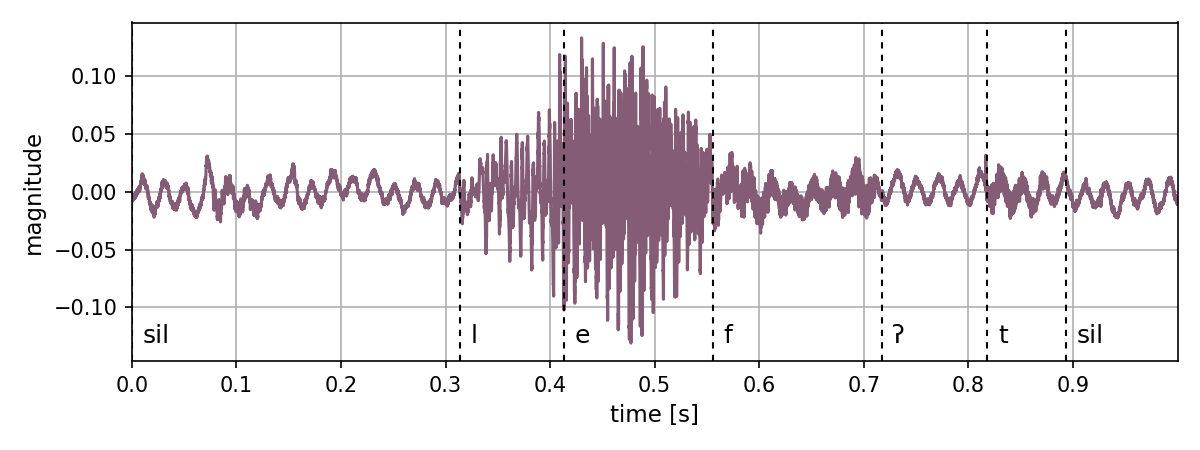
\includegraphics[width=0.45\textwidth]{./3_signal/figs/signal_raw_showcase_left0}}
    \subfigure[right]{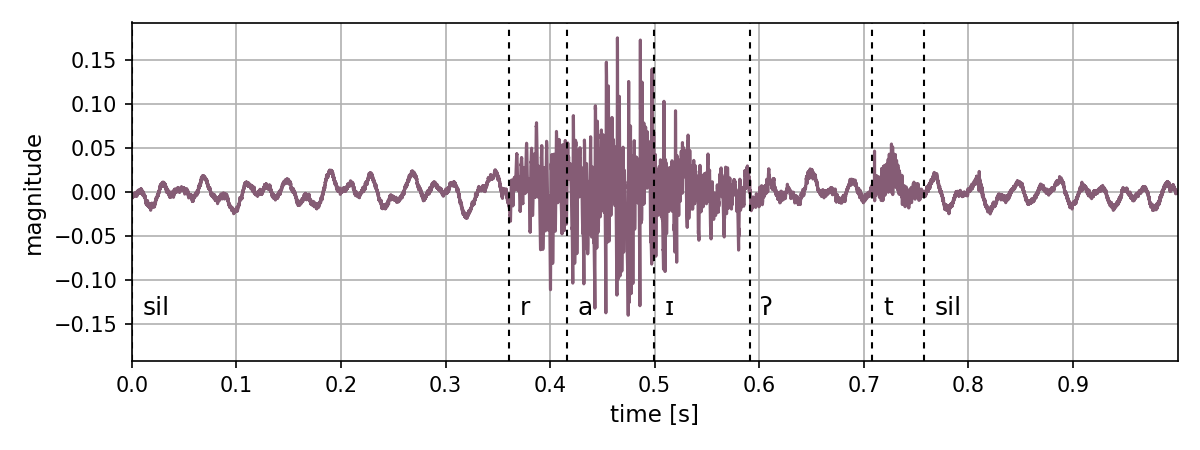
\includegraphics[width=0.45\textwidth]{./3_signal/figs/signal_raw_showcase_right0}}
    \subfigure[up]{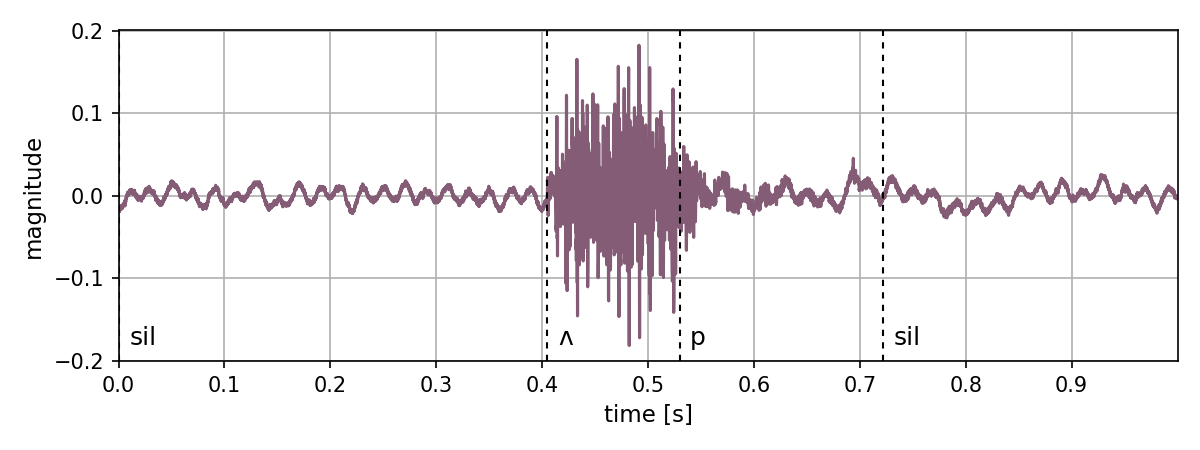
\includegraphics[width=0.45\textwidth]{./3_signal/figs/signal_raw_showcase_up0}}
    \subfigure[down]{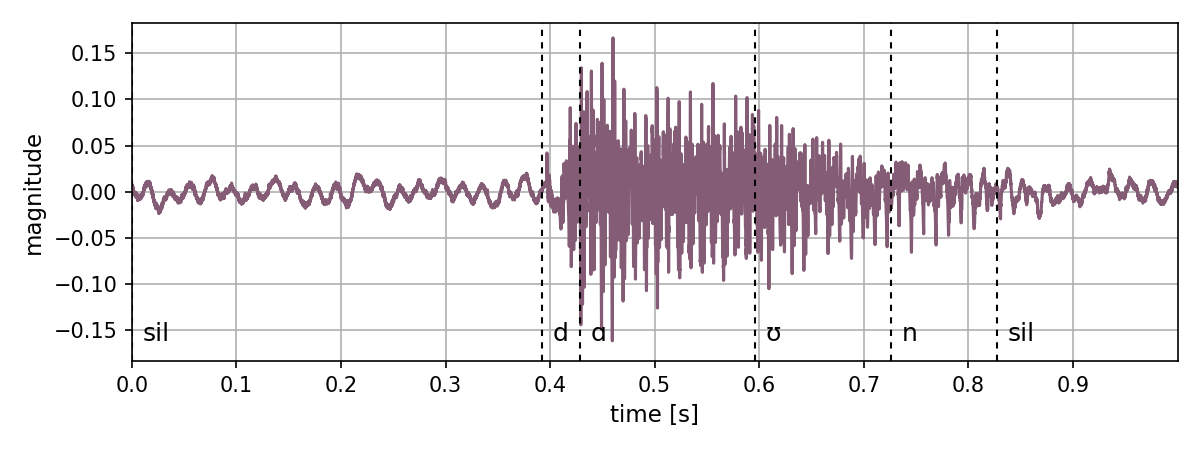
\includegraphics[width=0.45\textwidth]{./3_signal/figs/signal_raw_showcase_down0}}
    \subfigure[go]{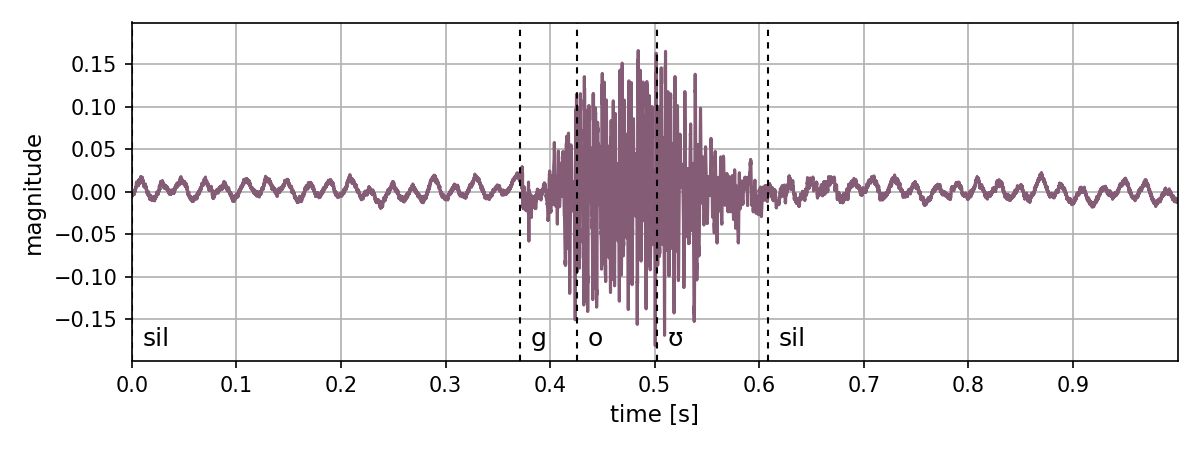
\includegraphics[width=0.45\textwidth]{./3_signal/figs/signal_raw_showcase_go0}}
  \caption{Raw audio waveform files, recorded by the author of this thesis with a simple consumer lavalier microphone.}
  \label{fig:signal_raw_showcase}
\end{figure}
\FloatBarrier
\noindent
From the shown raw audio files, one can estimate how long a speech command may take in terms of duration and see that usually a whole second is too much for a single speech command.
The pronunciation of words can of course deviate strongly in duration, but usually when commanding something it is preferred to speak short and well pronounced.
If a time interval of \SI{500}{\milli\second} is used to capture a speech command (this time interval is used in the feature extraction), it might happen that not every phoneme of the spoken words are captured. 
For instance this might happen often for words with glottal stops before consonants, for example the phoneme \enquote{t} in \enquote{left} or \enquote{right}, therefore the input features may only contain information of the first phonemes \enquote{lef} or \enquote{righ}.
But since Key Word Spotting (KWS) is restricted in its vocabulary and no similar words are included in the vocabulary, it should be no problem in distinguishing those.

Another important aspect is to detect the onset position of the speech commands on the time axis. 
It is easy to see in \rfig{signal_raw_showcase} where the spoken words are beginning and ending, but usually not all recordings are as clean as those.
There might be a huge noise level or background noise or cut away signals, so that the detection of the right onset position for the \SI{500}{\milli\second} time interval within the \SI{1}{\second} recordings is not always appropriate.
An intuitive method is to simply use the signal energy to determine the onset of the key words.
If the signal $x$ is windowed with the length of a \SI{500}{\milli\second} striding frame with sample length $N$, the energy of each windowed signal is calculated with:
\begin{equation}
  e_{w}(m) = \sum_{i=0}^{N-1} \abs{x[i + m]}^2
\end{equation}
with shift index $m = 0 \dots n - N + 1$, where $n$ is the number of sample of $x$.
The onset sample $o$ with the highest energy region is then determined by
\begin{equation}
  o = \underset{m}{\arg \max} \, e_{w}(m)
\end{equation}
for all windowed signal energies $e_{w}(m)$.

At last it should be noted, that the value range in the y-axis of audio recordings strongly depends on the microphone, amplifiers and post processing.
Therefore it is strongly recommended to normalize all recordings to a defined value range, with for instance the infinity norm:
\begin{equation}
  \hat{x} = \frac{x}{\norm{x}_\infty}
\end{equation}
so that the maximum or minimum value corresponds to either $+1$ or $-1$ and the signal range is defined between $[-1, 1]$.
% --
% spectrogram

\section{Spectral Features}\label{sec:signal_spec}
Spectral features, such as a spectrogram, are the most intuitive form to represent audio waveforms. 
It is possible to observe which frequencies are active at time instances.
Methodically this is done by shifting an \emph{analytic window} of time span $t_N$, on the time axis.
The time shifting has also a fixed time interval, denoted as \emph{hop time} $t_{h}$.
Both time parameters $t_N$ and $t_h$ can also be presented in samples by multiplying it with the sampling frequency $f_s$:

% samples
\begin{equation}
  \begin{split}
    N &= t_N \, f_s, \\
    h &= t_h \, f_s.
  \end{split}
\end{equation}
The audio samples contained by the analytic window of size $N$, are transformed with the Discrete Fourier Transform (DFT):

% DTFT
\begin{equation}\label{eq:signal_spec_dtft}
  \tilde{x}[k] = \sum_{n=0}^{N-1} x[n] \, e^{-j\frac{2 \pi n}{N}k}
\end{equation}
into the frequency space $\tilde{x}[k] \in \C$ with frequency index $k$ and discrete audio samples $x[n]$ with sample index $n$.
More conveniently, \req{signal_spec_dtft} can be written in matrix / vector notation with the DFT operator denoted as $\mathcal{F} \in \C^{k \times n}$:

% DFT matrix
\begin{equation}\label{eq:signal_spec_dtft_matrix}
  \tilde{x} = \mathcal{F}\, x \quad \mathrm{with} 
  \quad \mathcal{F}[p, q] = e^{-j\frac{2 \pi p}{N} q},
  \quad p,\, q = 0, 1, \dots k-1,\, 0, 1 \dots n-1.
\end{equation}
where $p$ and $q$ are row and column index in the matrix $\mathcal{F}$.
It follows that $\tilde{x} \in \C^k$ and $x \in \R^n$, where $n$ and $k$ denote here the dimension of input samples and frequency space respectively.

The length of the analytic window in samples $N$ is crucial for the frequency resolution and the lowest frequency that can be represented.
For example, the periodic time of a sound with $f=\SI{20}{\hertz}$ is $t=\frac{1}{f} = \SI{50}{\milli\second}$.
To represent a waveform it is necessary to have at least a quarter of its wavelength captured.
Within this thesis, the length of the analytic window is selected to \SI{25}{\milli\second}.

The other important parameter, the \emph{hop size} in samples of the hop time, by which the analytical window is shifted on the time axis, indicates the resolution in time and is especially important for changes within the audio data.
In applications like speech processing, the hop time should be selected so that the fastest pronounced phone and its transitions to other phones is captured within this time span with sufficient resolution.
Usually a hop time of $t_{h}=\SI{10}{\milli\second}$ is chosen for speech recognition tasks (also used within this thesis), but it could be extended to $t_{h}=\SI{20}{\milli\second}$, demonstrated in like in \cite{Peter2020}, for saving computations.

With those parameters in mind and $h$ denoted as hop size in samples and $N$ the length of the analytical window, the Short-Time Fourier Transform (STFT) for discrete time signals, can be computed as:

% stft
\begin{equation}\label{eq:signal_spec_stft}
    X[m, k] = \sum_{n=0}^{N-1} x[n + m] \, w[n] \, e^{-j\frac{2 \pi n}{N}k}, \qquad m = 0 \cdot h, \, 1 \cdot h, \, \dots, \, M \cdot h 
\end{equation}
note that $n$ is here the summation index, $w$ is a window function, such as the \emph{Hanning} window, $m$ indicates the hop index and $M$ is the maximum number of hops.
The maximum number of hops $M$ are all shifts of the analytic window by the hop size on the discrete time axis and can be computed as:

% hop
\begin{equation}\label{eq:signal_spec_hop}
  M = \frac{n-N}{h}
\end{equation}
where $n$ is here the length of the discrete time signal $x$.
A summary of the STFT parameters are shown in \rtab{signal_spec_stft}.

% stft params
% --
% stft params
\begin{table}[ht!]
\begin{center}
\caption{Parameters used for the STFT computation.}
\begin{tabular}{ M{4cm}  M{4cm}}
\toprule
\textbf{Parameter} & \textbf{Value} \\
\midrule
Sampling Frequency & \SI{16}{\kilo\hertz}\\
Analytic window size & \SI{25}{\milli\second}\\
Hop size & \SI{10}{\milli\second}\\
Window Function & Hanning\\
\bottomrule
\label{tab:signal_spec_stft}
\end{tabular}
\end{center}
\end{table}
\FloatBarrier
\noindent

A spectrogram $P \in \R^{m \times k}$ is simply the power spectrum of the STFT signal and is computed with:

% spec
\begin{equation}\label{eq:signal_spec_spec}
  P[m, k] = \abs{X[m, k]}^2.
\end{equation}
A spectrogram with linear representation is shown in \rfig{signal_spec_lin_examples}.

\begin{figure}[!ht]
  \centering
    \subfigure[left]{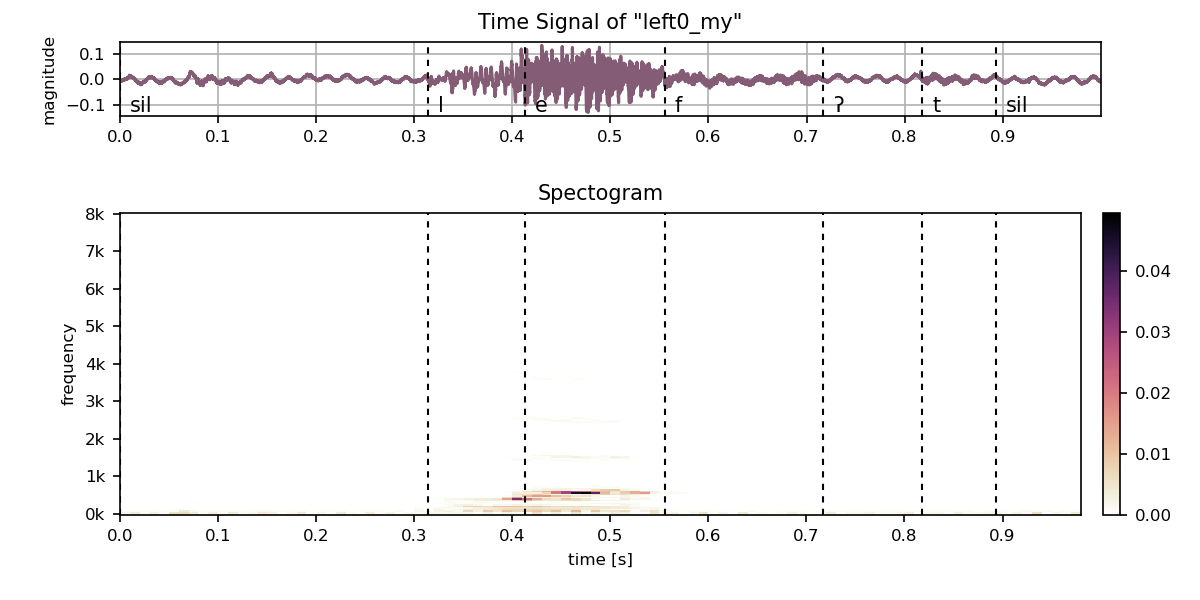
\includegraphics[width=0.45\textwidth]{./3_signal/figs/signal_spec-lin_left0_my}}
    \subfigure[right]{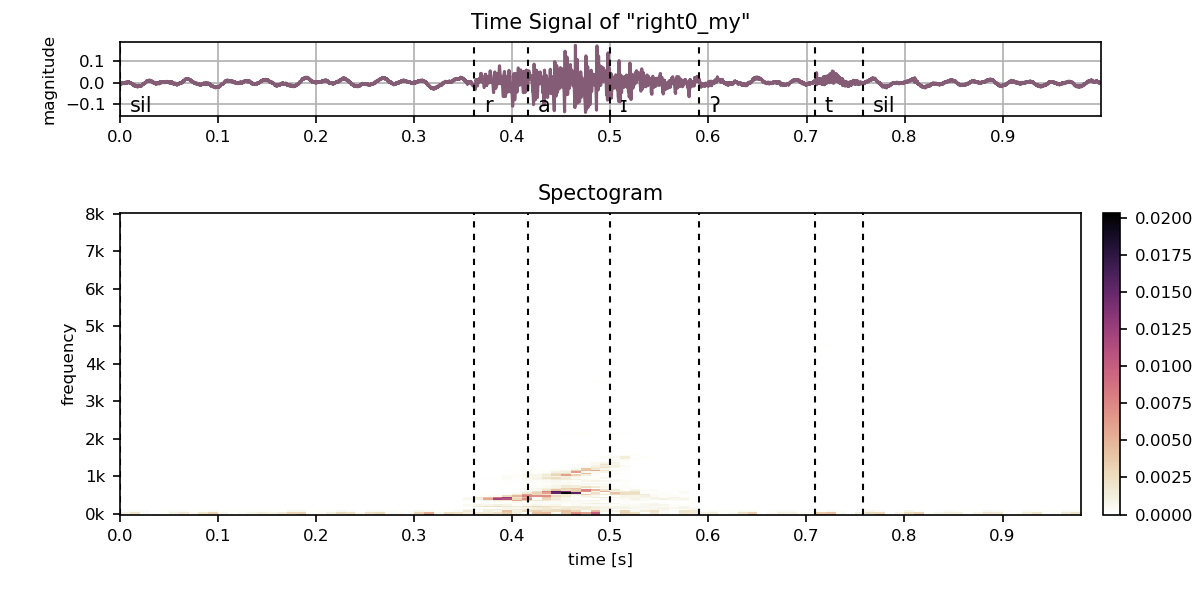
\includegraphics[width=0.45\textwidth]{./3_signal/figs/signal_spec-lin_right0_my}}
    \subfigure[up]{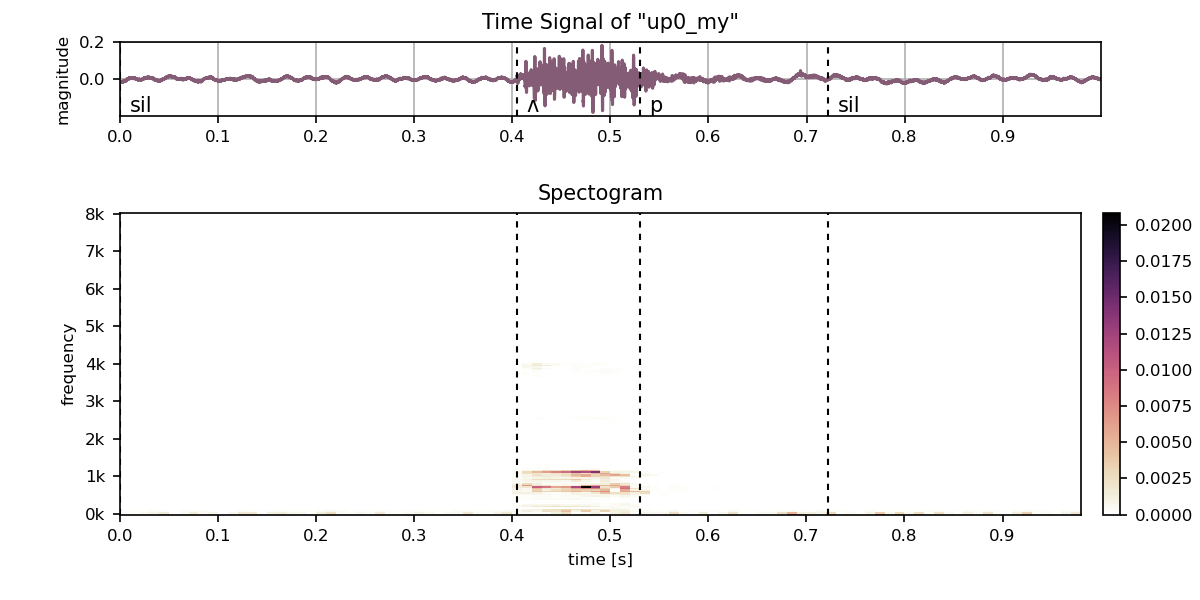
\includegraphics[width=0.45\textwidth]{./3_signal/figs/signal_spec-lin_up0_my}}
    \subfigure[down]{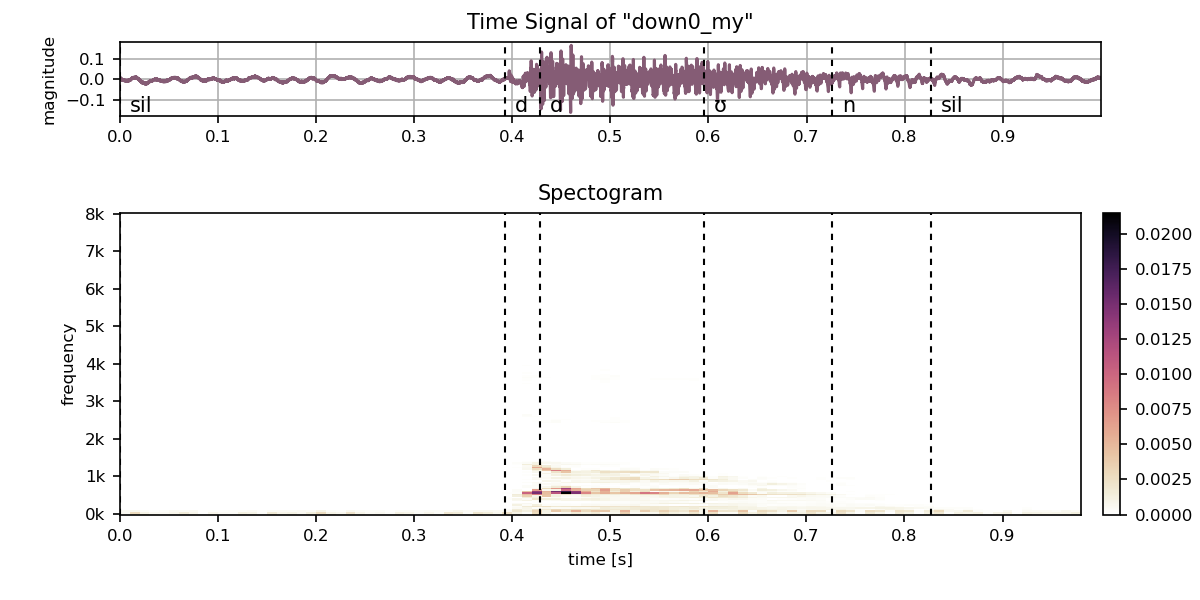
\includegraphics[width=0.45\textwidth]{./3_signal/figs/signal_spec-lin_down0_my}}
    \subfigure[go]{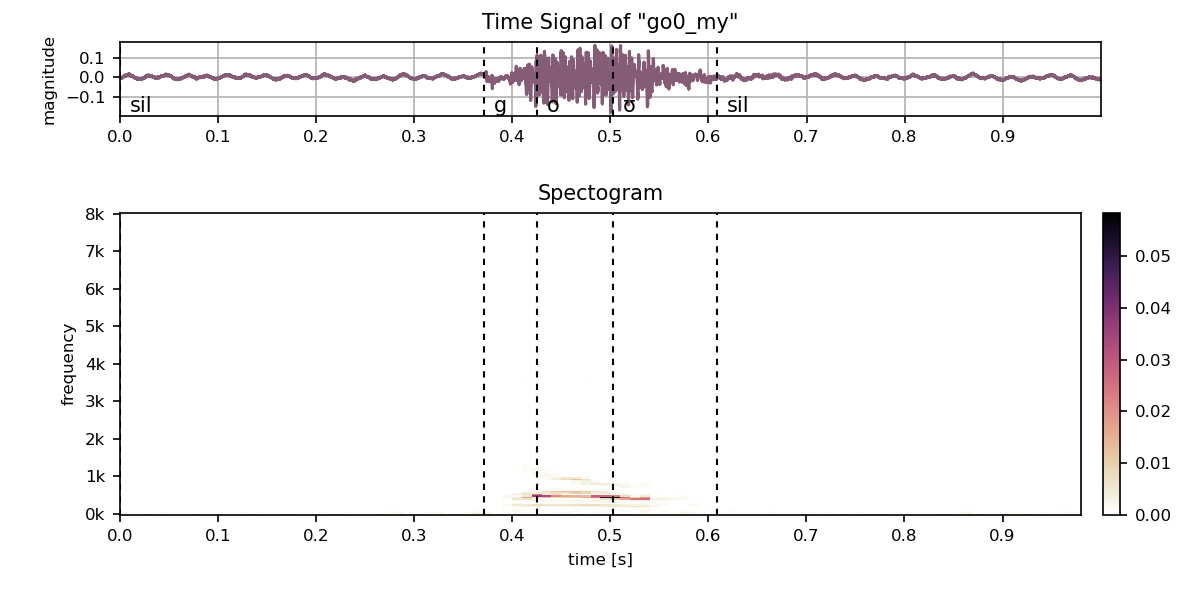
\includegraphics[width=0.45\textwidth]{./3_signal/figs/signal_spec-lin_go0_my}}
  \caption{Spectrogram linear scaled.}
  \label{fig:signal_spec_lin_examples}
\end{figure}
\FloatBarrier
\noindent

One can see here, that most of the energy of the signal is in the lower frequency regions under \SI{1}{\kilo\hertz}.
It is more interesting to transform the signal into the log scale with:

% log
\begin{equation}\label{eq:signal_spec_log}
  P_{DB}[m, k] = 10 \cdot \log{P[m, k]}
\end{equation}
so that small energies are visualized much better. 
The same examples with log scale are shown in \rfig{signal_spec_log_examples}.

\begin{figure}[!ht]
  \centering
    \subfigure[left]{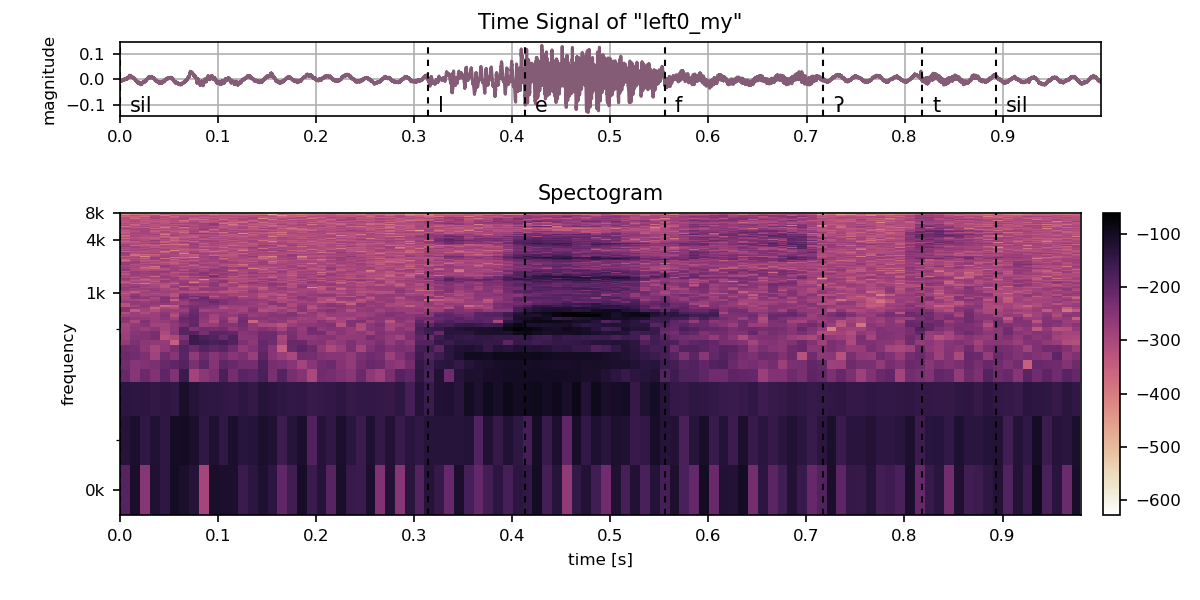
\includegraphics[width=0.45\textwidth]{./3_signal/figs/signal_spec-log_left0_my}}
    \subfigure[right]{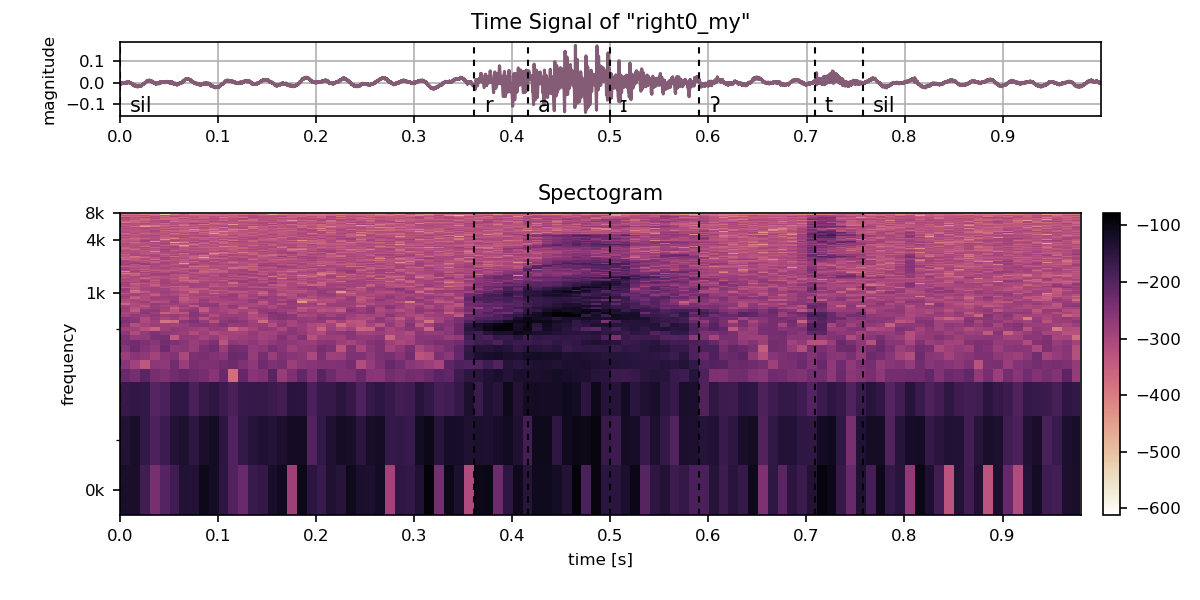
\includegraphics[width=0.45\textwidth]{./3_signal/figs/signal_spec-log_right0_my}}
    \subfigure[up]{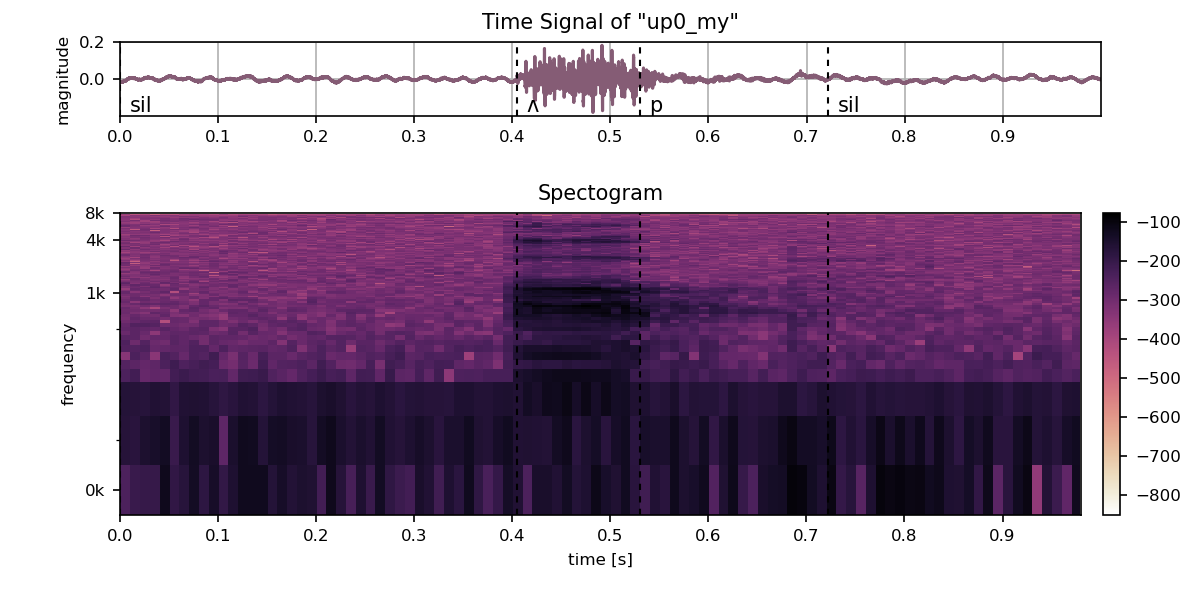
\includegraphics[width=0.45\textwidth]{./3_signal/figs/signal_spec-log_up0_my}}
    \subfigure[down]{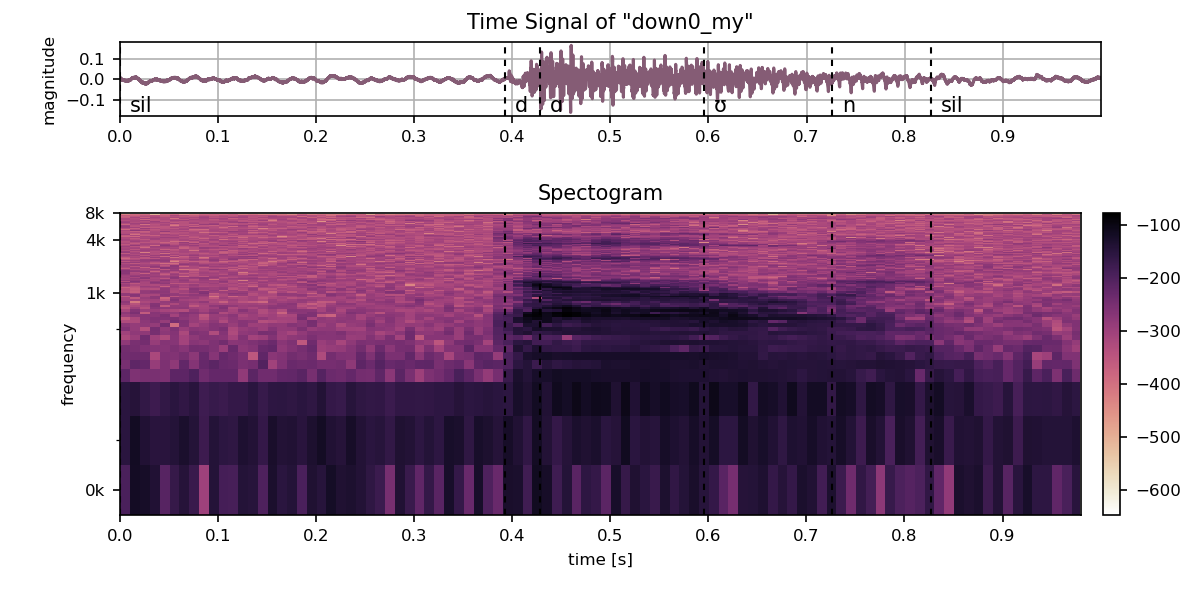
\includegraphics[width=0.45\textwidth]{./3_signal/figs/signal_spec-log_down0_my}}
    \subfigure[go]{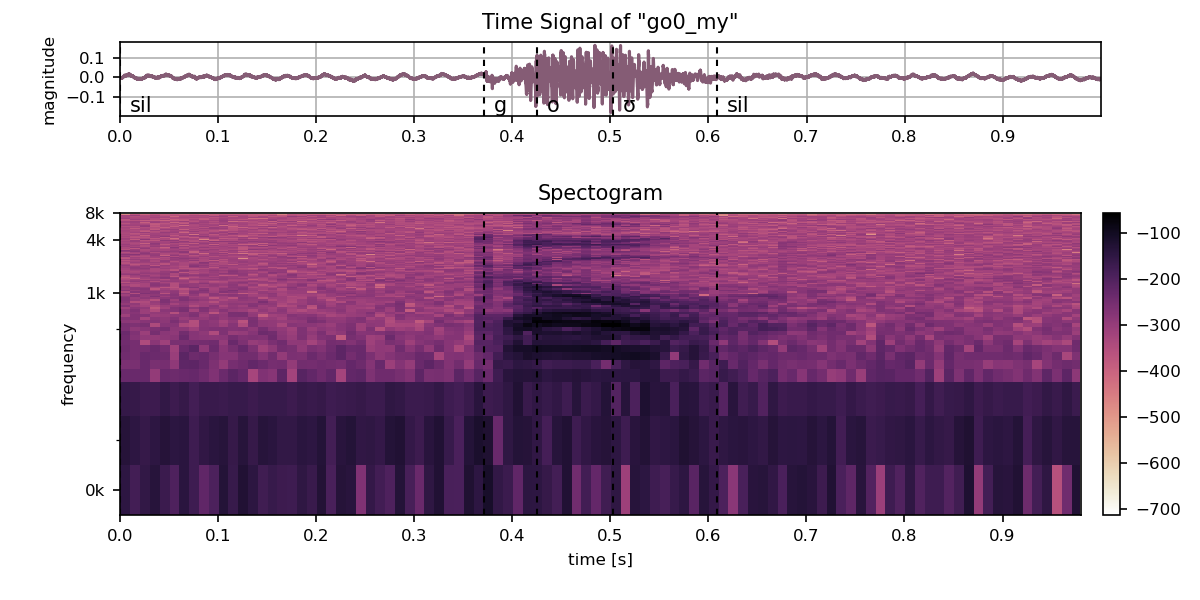
\includegraphics[width=0.45\textwidth]{./3_signal/figs/signal_spec-log_go0_my}}
  \caption{Spectrogram logarithmic scaled.}
  \label{fig:signal_spec_log_examples}
\end{figure}
\FloatBarrier
\noindent

Now it is possible to see some interesting structures and movements in the spectrograms in the frequency axis over time.
Still it is possible to improve the visualization of the spoken command words with a better compression scheme, such as the Mel Frequency Cepstral Coefficients, explained in the next section.
% --
% mfcc

\section{Mel Frequency Cepstral Coefficients}\label{sec:signal_mfcc}
Most commonly the Mel Frequency Cepstral Coefficients (MFCC) are used as input features for Neural Network classifications tasks of audio data.
It is described why they are good features and how they can be visualized to understand them better.

\begin{figure}[!ht]
  \centering
    \subfigure[left]{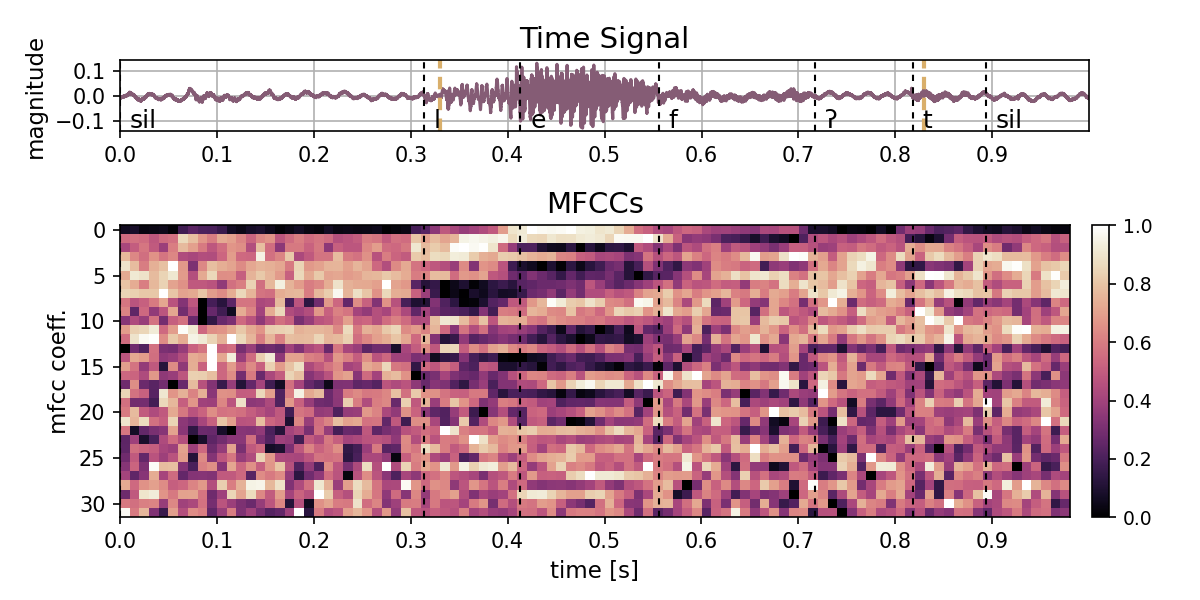
\includegraphics[width=0.45\textwidth]{./3_signal/figs/signal_mfcc_left0_my}}
    \subfigure[right]{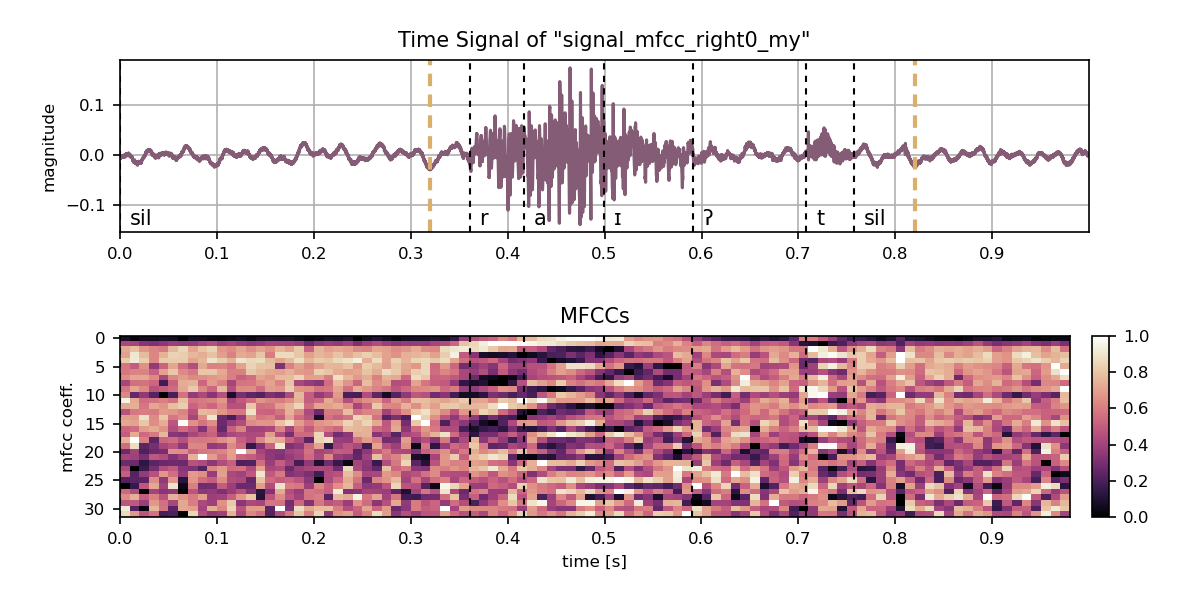
\includegraphics[width=0.45\textwidth]{./3_signal/figs/signal_mfcc_right0_my}}
    \subfigure[up]{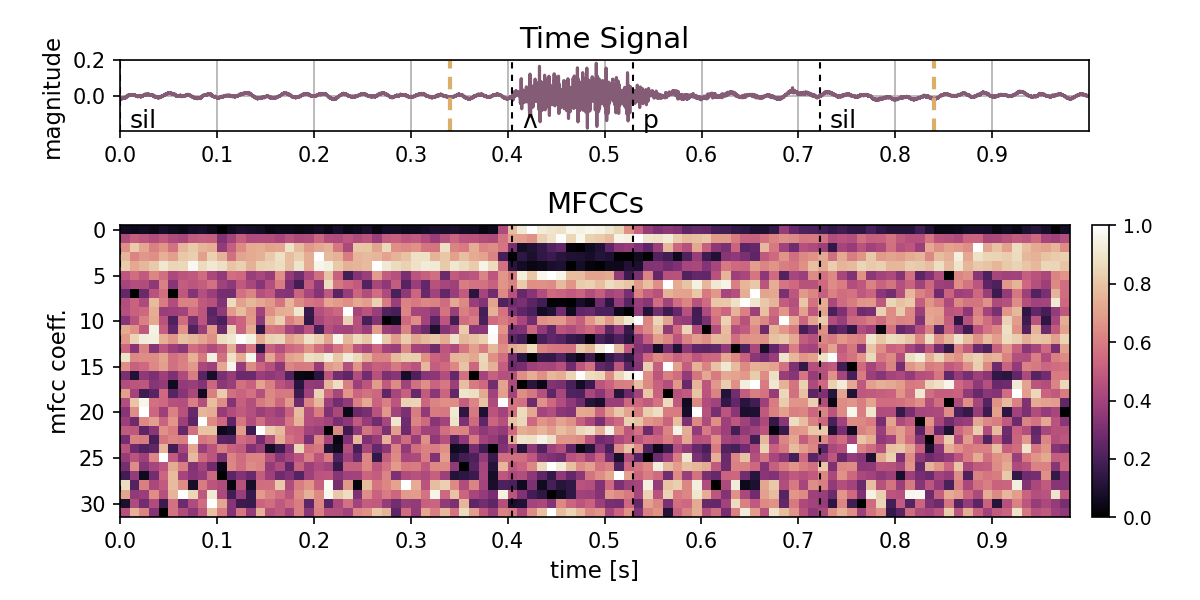
\includegraphics[width=0.45\textwidth]{./3_signal/figs/signal_mfcc_up0_my}}
    \subfigure[down]{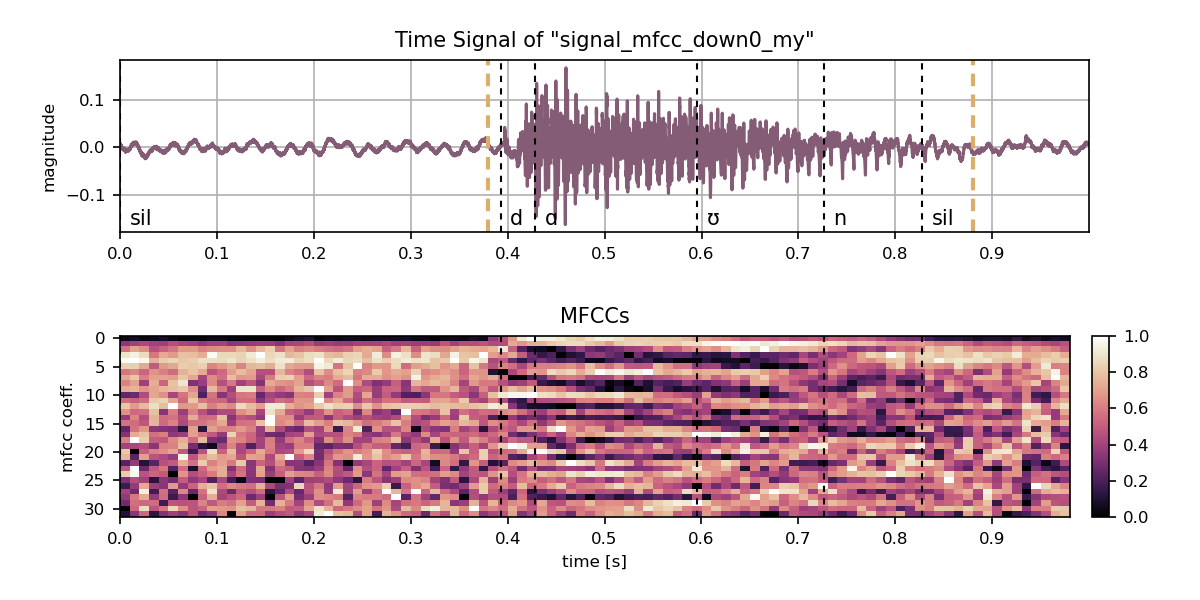
\includegraphics[width=0.45\textwidth]{./3_signal/figs/signal_mfcc_down0_my}}
    \subfigure[go]{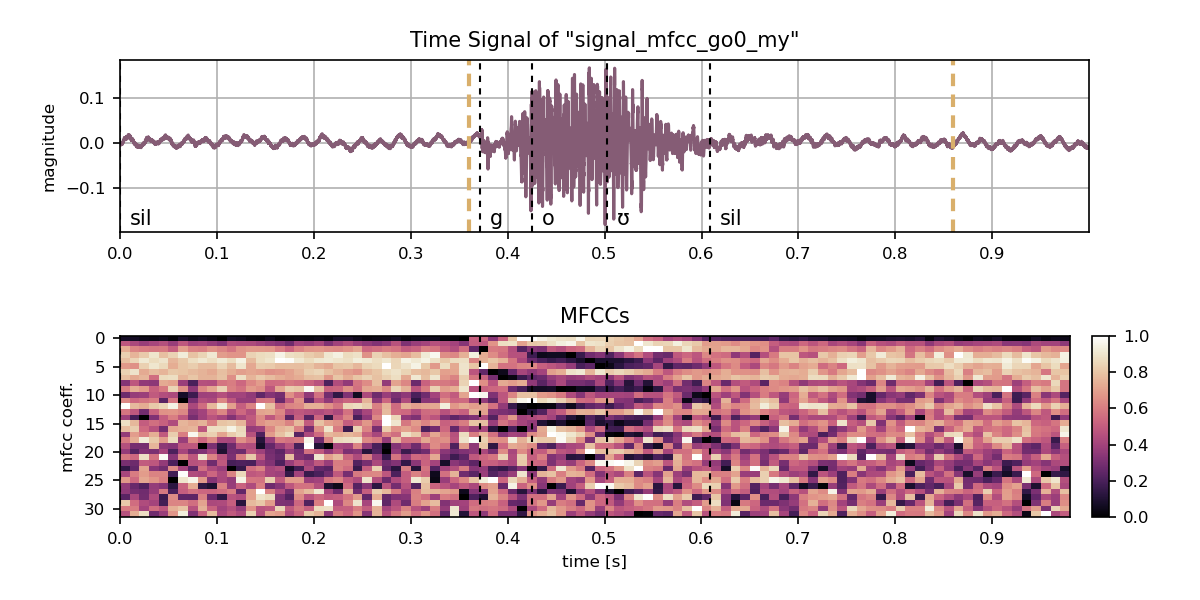
\includegraphics[width=0.45\textwidth]{./3_signal/figs/signal_mfcc_go0_my}}
  \caption{MFCC visualized with frame-based normalization.}
  \label{fig:signal_mfcc_examples}
\end{figure}
\FloatBarrier
\noindent

\subsection{The Idea behind}
To comprehend the success and wide use of MFCCs features in Neural Networks and other machine learning applications, it is necessary to understand its processing scheme:
Raw audio samples are transformed into the frequency domain with the Short-Time Fourier Transform (STFT).
Afterwards the power spectrum of the STFT is segmented in frequency bands (along the frequency dimension) done by a filter bank.
The filter bands are spaced in equidistant mel frequencies,
where the term mel frequencies is referred to the non-linear relationship between the mel and frequency scale.
The mel scale was developed in psychoacoustic experiments, where researchers found out, that high frequency sounds are perceived lower by humans, than they actual are (in musical hearing). For instance, in the musical sense an octave is the doubling of the frequency, but for human hearing it is strongly different and frequency doubling is not enough so that the same pitch is perceived.
This effect usually becomes imminent over \SI{500}{\hertz}.
As conclusion the mel scale is suited human hearing perception and taking equidistant mel bands is a reasonable decision.
In the following a logarithmic scaling in the value space of the power spectrum is done, which is also related to human hearing.
The last step is not that straight forward, but is a technique widely used in image processing, called the Discrete Cosine Transform (DCT).
It is only to mention that is some kind of decorrelation process, so that different filter bands are mixed together.

This processing steps seem rather complicated in the beginning, but are in fact nothing else but consecutive steps of appropriate scaling and data compression.
It is to mention that Neural Networks usually are able to handle large amounts of input features, but it is always preferable to decrease the input size, such that the model size of the Neural Network can be decreased same-wise.
Therefore it becomes more clear, why frequencies are put into certain frequency bands, are log scaled and as last step decorrelated with a method like the DCT.

\subsection{Processing Pipeline in detail}
The frequency spectrum is spitted into filter bands, done by triangular window functions.
Those window functions must have a fixed length on the mel space (equidistant mel bands), that results in different spacings in
the frequency space.
The mel - frequency relation can be approximated with:
\begin{equation}\label{eq:signal_mfcc_mel}
  m(f) = 2595 \cdot \log_{10} \left(1 + \frac{f}{700} \right) 
\end{equation}
where $m$ is the result in mel scale as function of the frequency $f$.
The mel scale plotted against the frequency scale is illustrated in \rfig{signal_mfcc_mel_scale}
\begin{figure}[!ht]
  \centering
  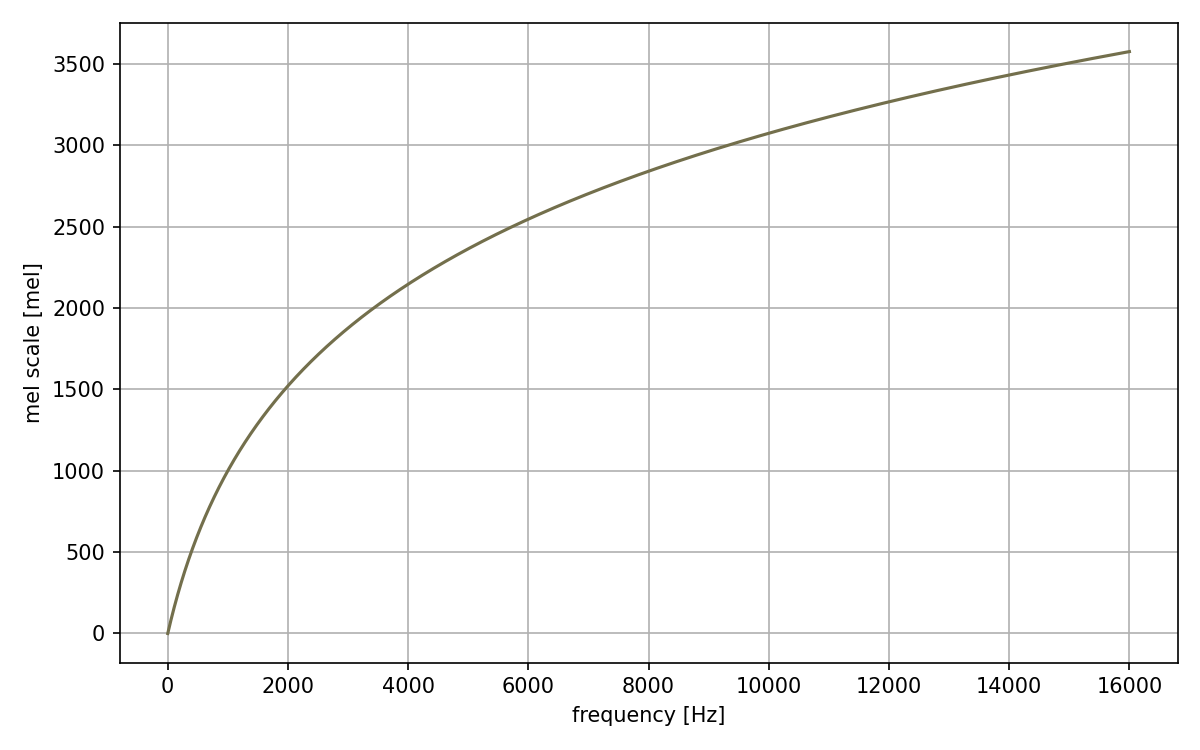
\includegraphics[width=0.40\textwidth]{./3_signal/figs/signal_mfcc_mel_scale}
  \caption{Mel scale as function of the frequency in a range of [0, \SI{16}{\kilo\hertz}].}
  \label{fig:signal_mfcc_mel_scale}
\end{figure}
\FloatBarrier
\noindent


The mel and frequency window functions are shown in \rfig{filter_bands}.
\begin{figure}[!ht]
  \centering
  \subfigure[mel space]{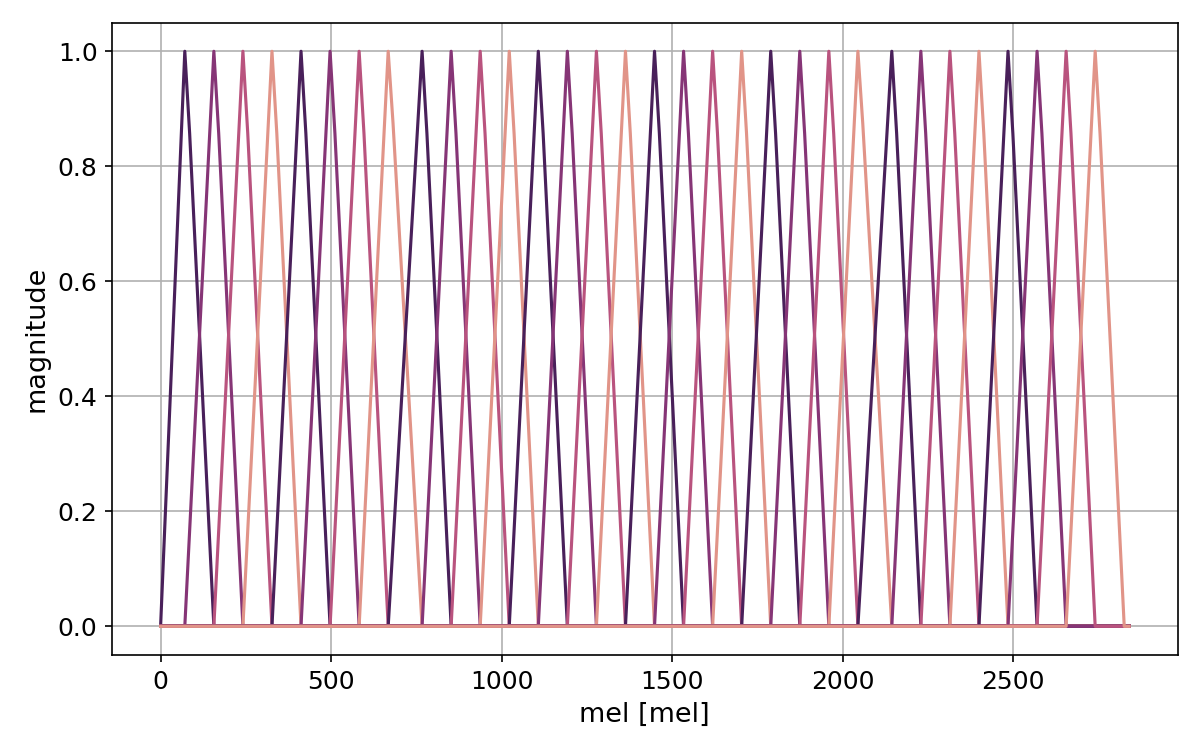
\includegraphics[width=0.40\textwidth]{./3_signal/figs/signal_mfcc_weights_mel}}
  \quad
  \subfigure[frequency space]{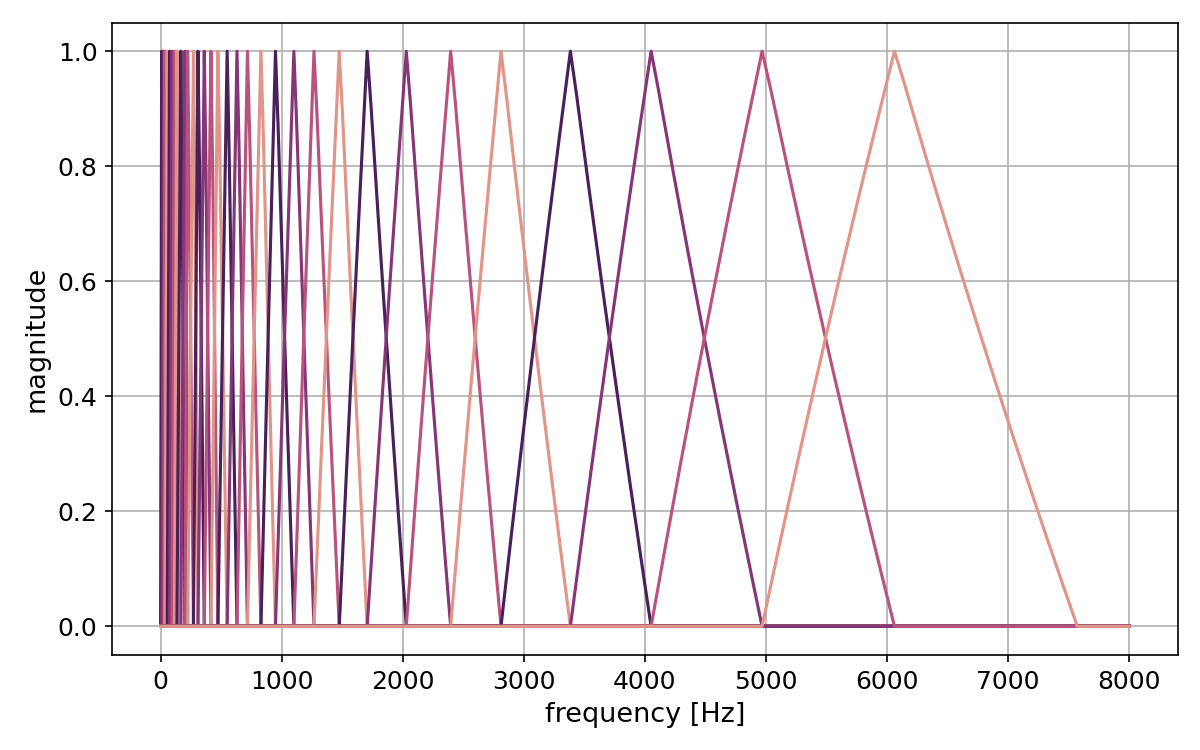
\includegraphics[width=0.40\textwidth]{./3_signal/figs/signal_mfcc_weights_f}}
  \caption{Equidistant mel filter bands with a total number of 32 bands.}
  \label{fig:filter_bands}
\end{figure}
\FloatBarrier
\noindent

The DCT is similar to the Fourier Transform and projects the input signal to a set of basis functions. 
These Basis functions are illustrated in \rfig{dct}
\begin{figure}[!ht]
  \centering
  \subfigure[DCT with continuous color scheme]{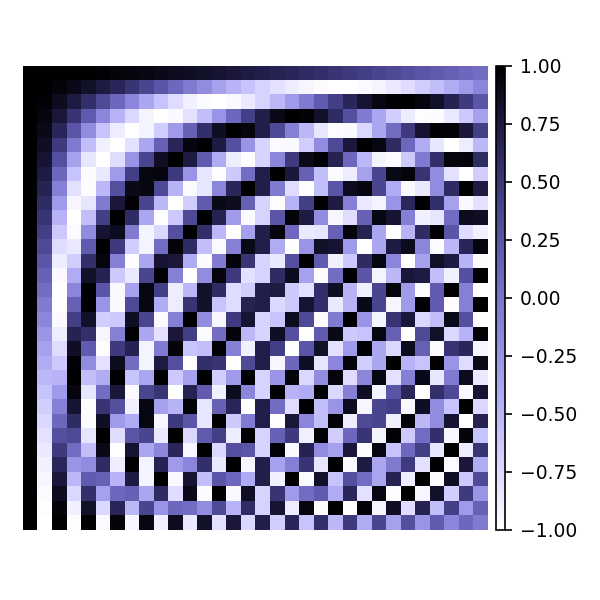
\includegraphics[width=0.40\textwidth]{./3_signal/figs/signal_mfcc_dct}}
  \quad
  \subfigure[DCT with diverging color scheme]{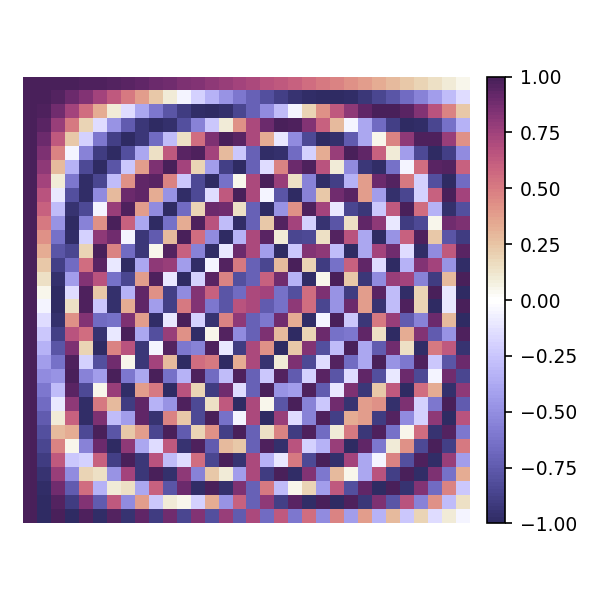
\includegraphics[width=0.40\textwidth]{./3_signal/figs/signal_mfcc_dct-div}}
  \caption{DCT matrix with 32 basis functions illustrated with a continuous and a diverging color scheme.}
  \label{fig:dct}
\end{figure}
\FloatBarrier
\noindent


\subsection{MFCC Feature Usage and Enhancement}
After the MFCCs are computed, they can be used as input features for Neural Networks. 
The important Question here is whether an feature enhancement can be done and if all those computed features are necessarily and meaningful for the training and evaluation success of Neural Networks. Usually not all MFCC coefficients are used as inputs, this is merely done to reduce the computational cost in case the accuracy does not suffer from it.
A good application is to compute 32 MFCC features (with 32 equidistant Mel filter bands) and use only the first 12 of them as inputs.
Further it is also possible to compute derivatives (in the time domain) of MFCC features, denoted as Deltas. 
Those derivatives are simple computed as frame difference of the MFCCs.
A second derivative of MFCC features, known as Double Deltas, are then the frame differences of the Deltas.
At last an energy feature can be computed from each of the MFCCs, Deltas and Double Deltas, each by its own and added to the feature vectors.
Those feature vectors can then be simply stacked at top of each other and used as feature inputs.
In this thesis the feature vectors are stacked as following:
\begin{enumerate}
    \item 12 MFCCs
    \item 1 Energy feature of the 12 MFCCs
    \item 12 Deltas
    \item 1 Energy feature of the 12 Deltas
    \item 12 Double Deltas
    \item 1 Energy feature of the 12 Double Deltas
\end{enumerate}
Which sums up to a 39-dimensional feature vector.

\subsection{Visualisation of MFCC features}
A good visualisation of MFCC features is the best way to understand them.
With this thought in mind, much time was spent to create a fitting visual representation of the MFCC features, but this was not an easy task.
MFCCs are not well intended for visualisations, since their individual coefficients value space, can be strongly different from each other.
For example, the first coefficient equals a summation of all filter bands and is therefore some kind of energy measure over all bands, while the other coefficients are weighted sum combinations of the filter bands.
This alone yields in totally different value spaces and value spaces should not differ that much, when features should be represented with colors.
Further it is to mention, that most of the signal energy will be in the lower frequency bands, which also impacts the value space of the individual coefficients a lot.
To show this difference in value space in a negative example in practise, the MFCCs of the self-recorded speech command waveform \enquote{left0.wav} is shown in \rfig{left0_mfcc_only}.

\begin{figure}[!ht]
  \centering
    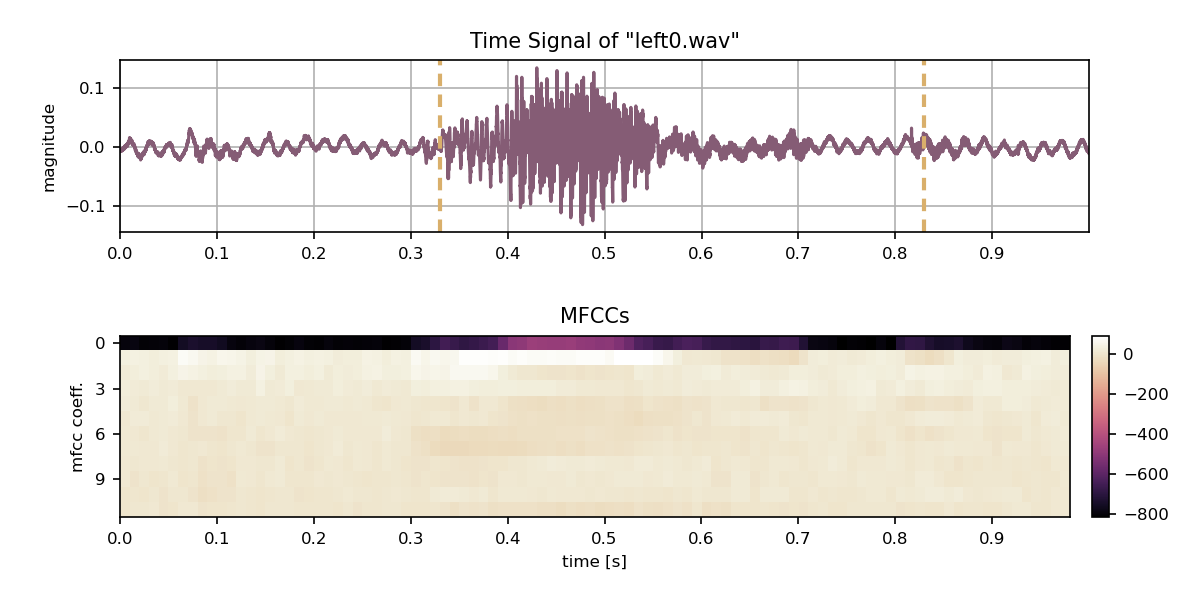
\includegraphics[width=0.75\textwidth]{./3_signal/figs/signal_mfcc_left0_mfcc_only.png}
  \caption{Bad visualisation of the 12 MFCCs features extracted from \enquote{left0.wav}.}
  \label{fig:left0_mfcc_only}
\end{figure}
\FloatBarrier
\noindent
Not much structure of the MFCCs can be seen here, due to the vast value difference of the first coefficient. At least the first coefficient shows, where the center of signal energy is placed on the time scale, but other than that, this visualisation is worthless.
Another very bad visualisation is shown by computing the 39 MFCC feature vectors (with Deltas, Double Deltas and Energies) in \rfig{left0_no_order}.

\begin{figure}[!ht]
  \centering
    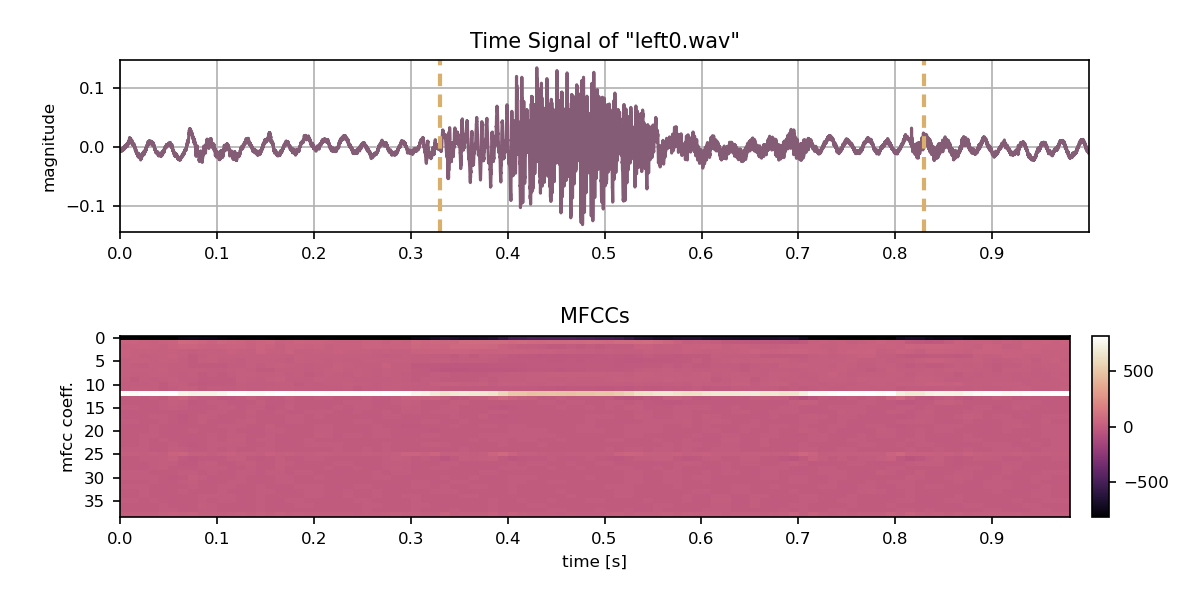
\includegraphics[width=0.75\textwidth]{./3_signal/figs/signal_mfcc_left0_no_order_norm0.png}
  \caption{Very bad visualisation of 39 MFCC features extracted from \enquote{left0.wav}.}
  \label{fig:left0_no_order}
\end{figure}
\FloatBarrier
\noindent
There appears an even greater gap of different value spaces and even less is seen.
One very easy solution is to show the features in different value groups. For instance the first coefficient and its deltas is in one group, the other coefficients in another and the deltas and energies are separated as well in own groups. Now we actually can see some structure in the visualisations, shown in \rfig{left0_order}.

\begin{figure}[!ht]
  \centering
    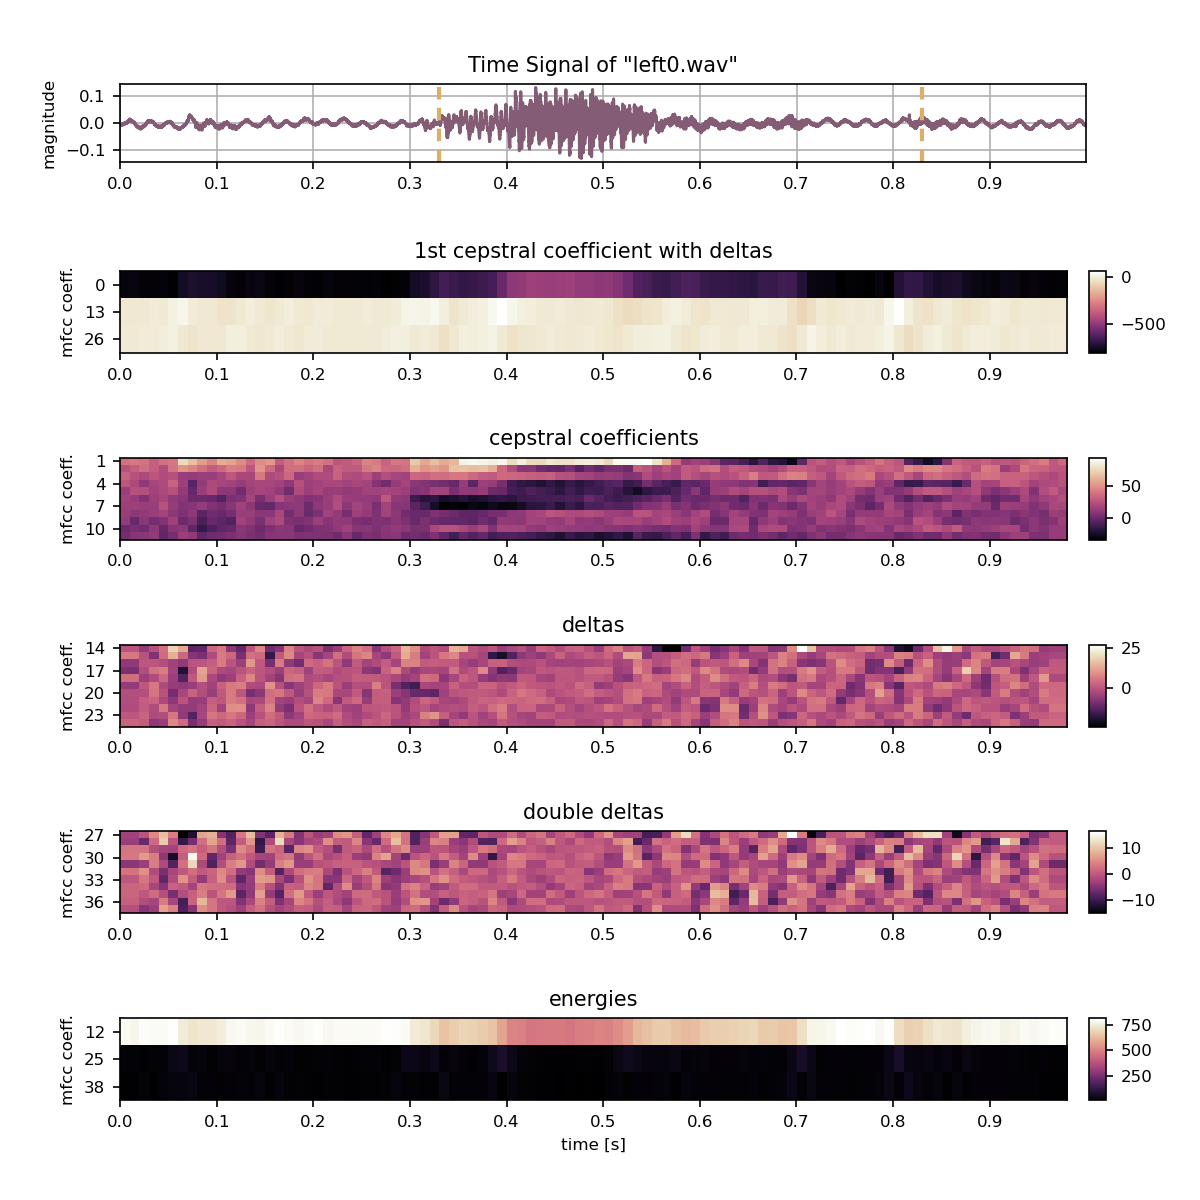
\includegraphics[width=0.75\textwidth]{./3_signal/figs/signal_mfcc_left0_norm0.png}
  \caption{Good visualisation of 39 MFCC features extracted from \enquote{left0.wav} with own value groupings.}
  \label{fig:left0_order}
\end{figure}
\FloatBarrier
\noindent
Another way to improve the visualisation is to normalize the feature vectors over their each own frame dimension with the infinity norm. This will yield a value space of $[0, 1]$ for each feature vector. With this, the visualisation of the 39 MFCC of \enquote{left0.wav} is shown in \rfig{left0_order},

\begin{figure}[!ht]
  \centering
    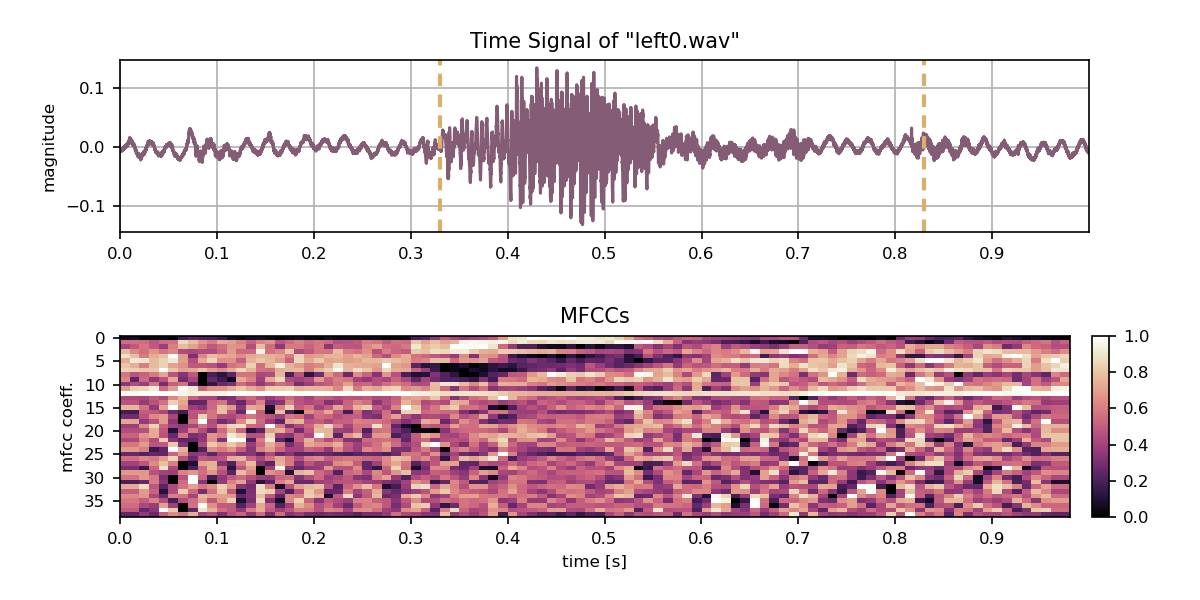
\includegraphics[width=0.75\textwidth]{./3_signal/figs/signal_mfcc_left0_no_order_norm1.png}
  \caption{Normalisation of 39 MFCC features extracted from \enquote{left0.wav}.}
  \label{fig:left0_no_order_norm1}
\end{figure}
\FloatBarrier
\noindent
or in an even better one shown in \rfig{left0_order_norm1}.

\begin{figure}[!ht]
  \centering
    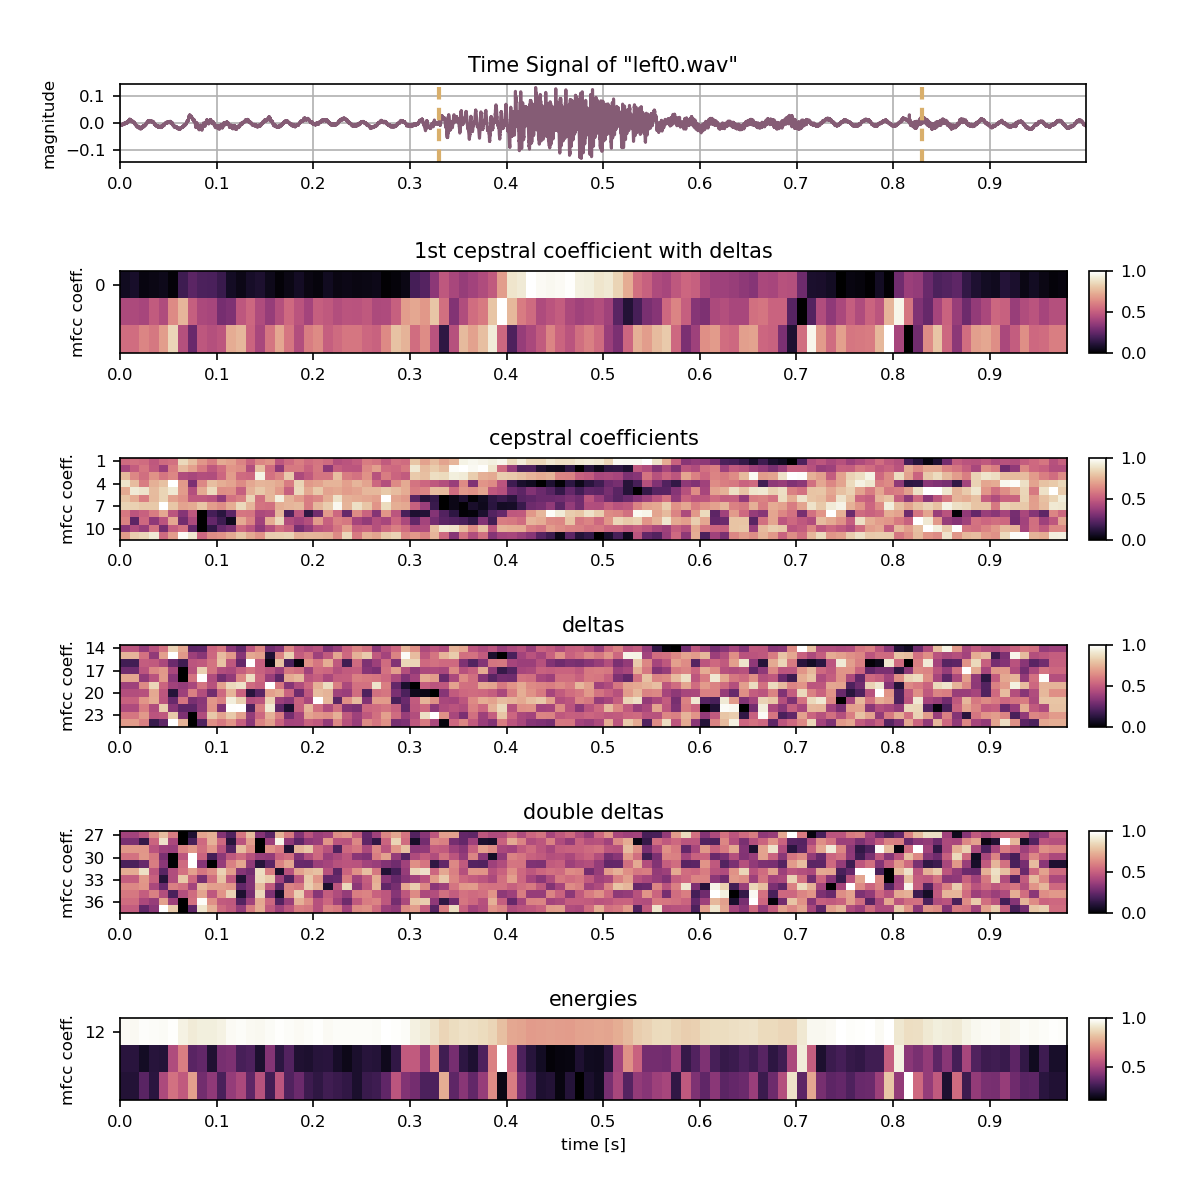
\includegraphics[width=0.75\textwidth]{./3_signal/figs/signal_mfcc_left0_order_norm1.png}
  \caption{Normalisation of 39 MFCC features extracted from \enquote{left0.wav} with groups.}
  \label{fig:left0_order_norm1}
\end{figure}
\FloatBarrier
\noindent
As conclusion, the normalisation in the frame space is an interesting aspect to improve the visualisation of the MFCC features, 
specifically for the cepstral coefficients and the energy features (not the deltas).
Exactly this nice representation was motivating to explore normalisation of feature for Neural Network inputs.
However this is a very crucial thing to do. A normalisation relatives important structures within the feature space and it cannot really be answered if this is a good thing or not.
One more research question arises here: Is it possible to use normalisation for the features as inputs to Neural Networks and what are the results to the accuracy and training of the models.


% --
% Neural Network Architectures

\chapter{Neural Networks}\label{sec:nn}
This chapter contains the theoretical foundations of developing a Key Word Spotting system with neural networks for Video Games. 
In particular the signal processing and feature extraction is explained and visualized with many examples.
The same holds fo the machine learning part were central concepts of applied methods are discussed and shown.
At last it is important and has to be considered when building a video game with speech command inputs.

% ml
% --
% Neural Network Architectures

\section{Neural Network Architectures}\label{sec:nn_arch}
All Neural Network Architectures evaluated within this thesis are presented here.
%There will be a general classification between Neural Network Architectures by Convolutional Neural Networks, Adversarial Neural Networks ...
In general the architectures can be differentiated between:
\begin{enumerate}
	\item Convolutional Neural Networks
	\item Adversarial Neural Networks
	\item Wavenets
\end{enumerate}
The term Convolutional Neural Networks here consists of all architectures consisting of at least one convolutional layer and the intention to simply classify each speech commands from each other. 
Therefore the output of a Convolutional net is of size of the amount of speech commands and usually has some kind of probability distribution or energy equivalence.

With Adversarial Neural Networks all architectures are meant, with at least two separate Neural Network Architectures, e.g. a Discriminator and a Generator Network and the intention to outperform the other Network in a task where both play a game against each other.
The word game here, is used in the sense of Game Theory, where the goal is to find an equilibrium state where both players are equally satisfied with the state.

An overview of all models is shown in \rtab{nn_arch_overview} with abbreviations in \rtab{nn_arch_abbreviation}.
\begin{table}[ht!]
\begin{center}
\caption{Network Architectures Abbreviations}
\begin{tabular}{ M{2.5cm}  M{10cm} }
\toprule
\textbf{Abbreviations} & \textbf{Meaning}\\
\midrule
c[0-9] & convolutional layer with layer number\\
f[0-9] & feed forward fully connected layer with layer number\\
m[0-9] & max pooling layer layer with layer number\\
ch & input channel number for mfccs it is usually 1\\
fs & frame size (usually 50 -> 50ms)\\
ms & feature size (mfcc), depends on feature selection\\
cf & output number of last flattened convolutional layer\\
cl & number of class labels\\
\bottomrule
\label{tab:nn_arch_abbreviation}
\end{tabular}
\end{center}
\end{table}
\FloatBarrier
\noindent
\begin{table}[ht!]
\begin{center}
\caption{Network Architectures Overview with reference names}
\begin{tabular}{ M{2.5cm}  M{2.1cm}  M{2.1cm} M{2.1cm} M{2.5cm}}
\toprule
%\multicolumn{4}{c}{\textbf{Feature Groups}} & \multicolumn{2}{c}{\textbf{Accuracy}} \\
\textbf{Reference name} & \textbf{Feature maps} & \textbf{Kernel sizes} & \textbf{Strides} & \textbf{Feed Forward} \\
\midrule
conv-trad & c1: (ch, 64) c2: (64, 64) & c1: (4, 20) mp: (2, 4) c2: (2, 4) & c1: (1, 1) mp: (2, 4) c2: (1, 1) & f1: (cf, 32) \quad f2: (32, 128) f3: (128, cl)\\
\midrule
conv-fstride & c1: (ch, 54) & c1: (8, fs) & c1: (4, 1) & f1: (cf, 32) \quad f2: (32, 128) \quad f3: (128, 128) \quad f4: (128, cl)\\
\midrule
conv-encoder-fc1 & c1: (ch, 48) \quad c2: (48, 8) & c1: (ms, 20) \quad c2: (1, 5) & c1: (1, 1) \quad c2: (1, 1) & f1: (cf, cl)\\
\midrule
conv-encoder-fc3 & c1: (ch, 48) \quad c2: (48, 8) & c1: (ms, 20) \quad c2: (1, 5) & c1: (1, 1) \quad c2: (1, 1) & f1: (cf, 64) \quad f2: (64, 32) \quad f3: (32, l)\\
\bottomrule
\label{tab:nn_arch_overview}
\end{tabular}
\end{center}
\end{table}
\FloatBarrier
\noindent


% --
% adversarial

\section{Adversarial Training Theory}\label{sec:nn_adv}
Working with adversarial Neural Networks is quite interesting, as two separate Networks are challenge themselves against each other to improve their performance.
The paper from Goodfellow et. al. \cite{Goodfellow2014} describes a game between two Neural Networks (players), where one player has the role of creating fakes and the other must determine if it is real or fake.
The Network who creates fakes is called Generator (G) and the other Network who has to decide about fake or not is called Discriminator (D).
The Generators goal is to create fakes that look like reals, so that D makes mistakes and classifies a fake as a real.
On the other hand the Discriminator must also constantly improving itself, so that fakes from G can be detected and sorted out from the reals.

This approach works remarkably well to create a generative network able to produce fakes that are astonishing similar to real ones.
In the mentioned paper, this was applied to images and not for audio data.
But if the audio waveform is presented as spectogram or mfcc with fixed frame size, it can be seen as an image, where one dimension is time and the other frequency.

So far a generative network does only produce fake images and a discriminative network can only output a one dimensional (probability) output, to decide if it is fake or not.

The idea now is not to use either of these networks, but to use transfer learning in the sense to reuse the convolutional layers both networks achieved during their game (training).
The weights of those convolutional layers are then transfered to another network with classification purpose on multiple labels.

\subsection{Questions that arise}
There are several questions that arise regarding Adversarial Training:
\begin{enumerate}[label={Q.\textgoth{A}.\arabic*)}, leftmargin=1.4cm]
  \item Does the Network Architecture of G and D have to be the same but transposed?
  \item Does the value space of in and outputs, for D and G respectively, have to be limited e.g. [0, 1] done by e.g. frame normalization, or sigmoid output?
  \item What loss function works well for training?
  \item How long should be trained?
  \item When transfering weights to another network, should the weights from G or D be transfered?
  \item Does the classification network has to adapt the parameters from the transfered weights?
  \item Whats the benefit of all this?
\end{enumerate}

To illustrate the idea an example is shown of the labels L5 (left, right, up, down, go).

The convolutional layer weights from the adversarial training of the individual labels, 
can be stacked together an used to initialize another network.
An example of this method is shown in \rfig{nn_adv_example}, where the initialization pattern changes to more elaborate structures and patterns to form good classification outputs. 
However the Basic Pattern from the adversarial training stays the same, which is a good sign, because then the network is accepting those trained weights and adapts them.

\begin{figure}[!ht]
  \centering
    \subfigure[c1 trained]{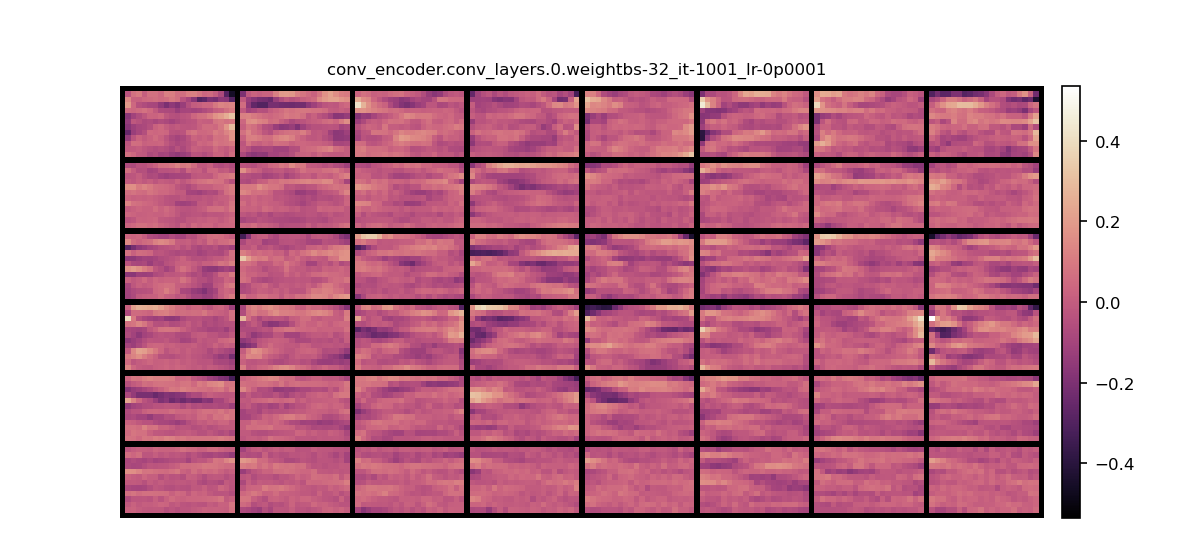
\includegraphics[width=0.45\textwidth]{./4_nn/figs/nn_adv_example_c0}}
    \subfigure[c1 init]{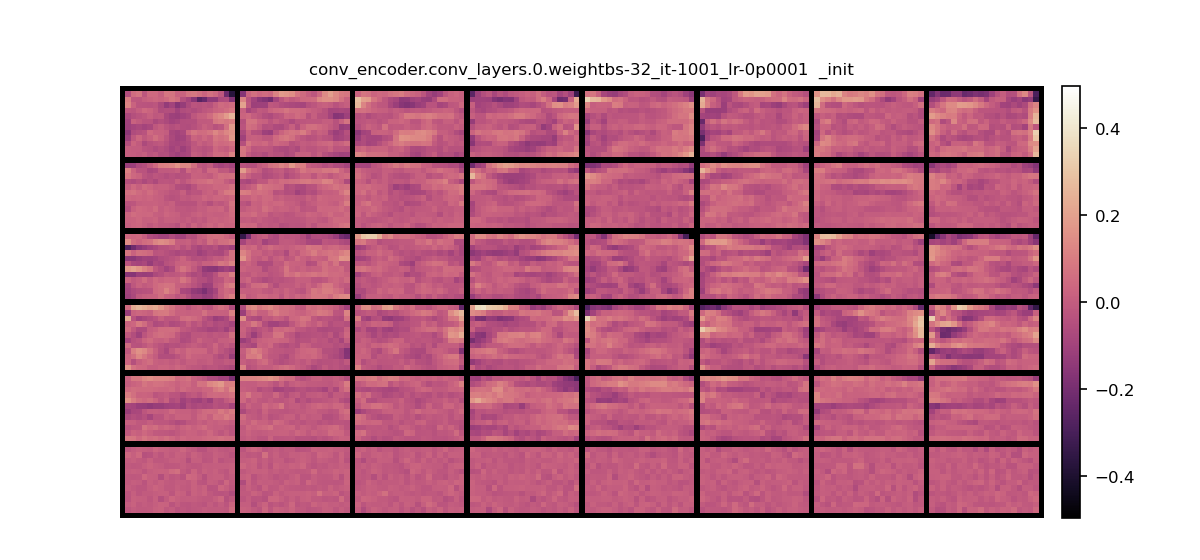
\includegraphics[width=0.45\textwidth]{./4_nn/figs/nn_adv_example_c0_init}}
    \subfigure[c2 trained]{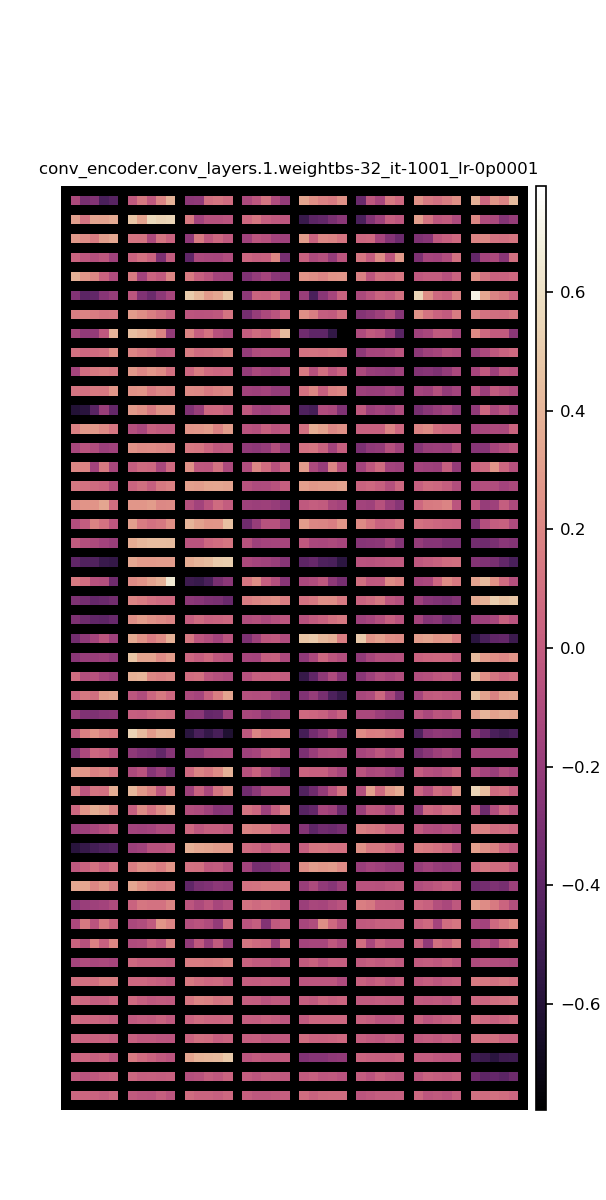
\includegraphics[height=0.45\textwidth]{./4_nn/figs/nn_adv_example_c1}}
    \quad
    \subfigure[c2 init]{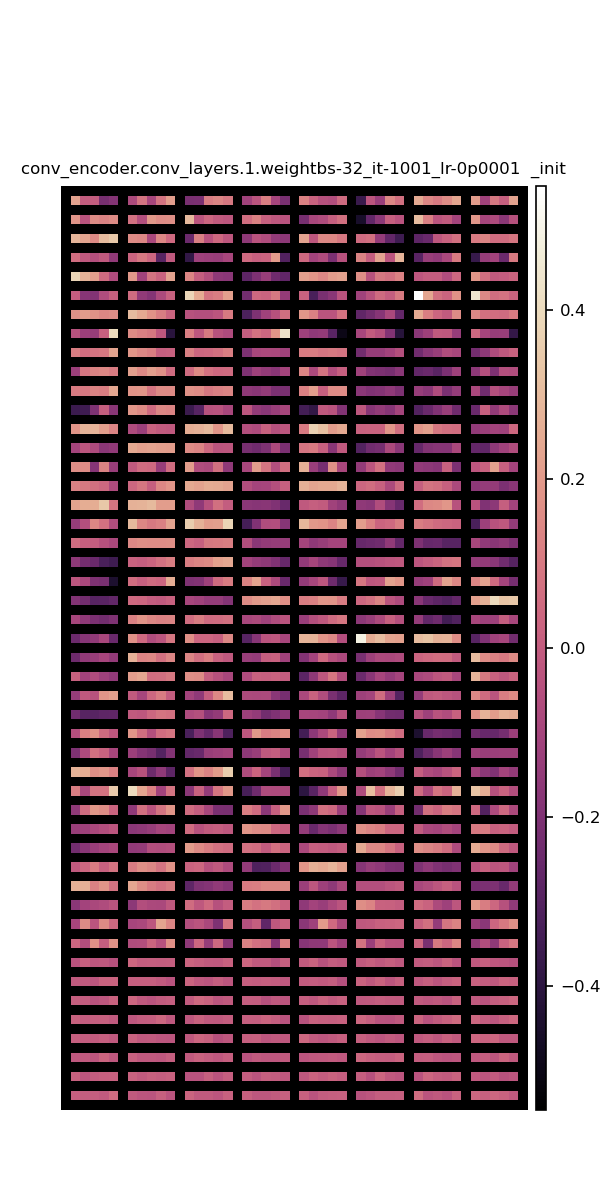
\includegraphics[height=0.45\textwidth]{./4_nn/figs/nn_adv_example_c1_init}}
  \caption{Adversarial Training Example: Convolutional layers pretrained with adversarial training on each label separately.}
  \label{fig:nn_adv_example}
\end{figure}
\FloatBarrier
\noindent

For this example in adversarial training, 8 feature maps of the first layer were used for each label, also they belong to the Generator Network G or decoder (dec). In Convolutional Networks, each previous layers feature map creates a new set of feature maps in the next layer.
An example of this label training is shown in \rfig{nn_adv_example_label} with feature maps [(1, 8), (8, 8)] of the convolutional layers

\begin{figure}[!ht]
  \centering
    \subfigure[\enquote{left} c1 from D]{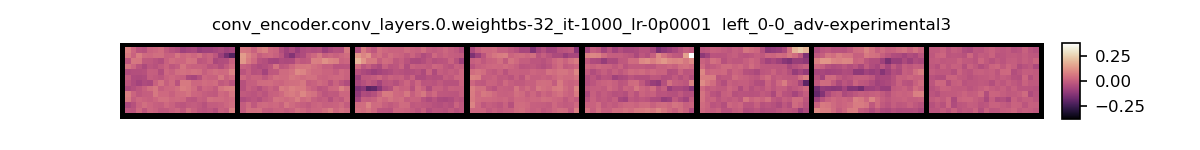
\includegraphics[width=0.45\textwidth]{./4_nn/figs/nn_adv_example_label_left_c0_enc}}
    \subfigure[\enquote{left} c1 from G]{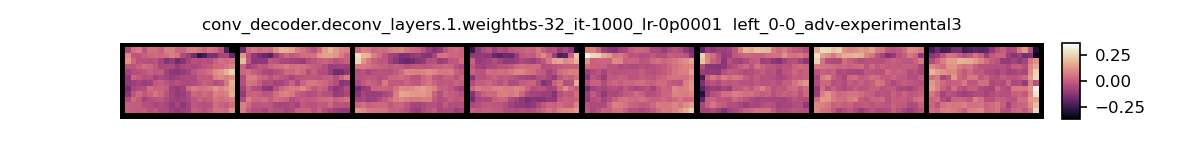
\includegraphics[width=0.45\textwidth]{./4_nn/figs/nn_adv_example_label_left_c0_dec}}
    \subfigure[\enquote{left} c2 from D]{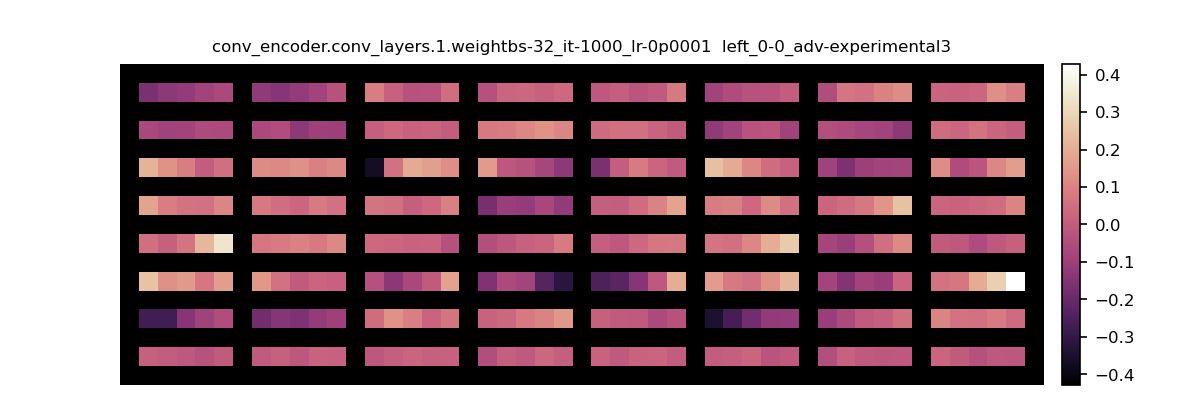
\includegraphics[width=0.3\textwidth]{./4_nn/figs/nn_adv_example_label_left_c1_enc}}
    \subfigure[\enquote{left} c2 from G]{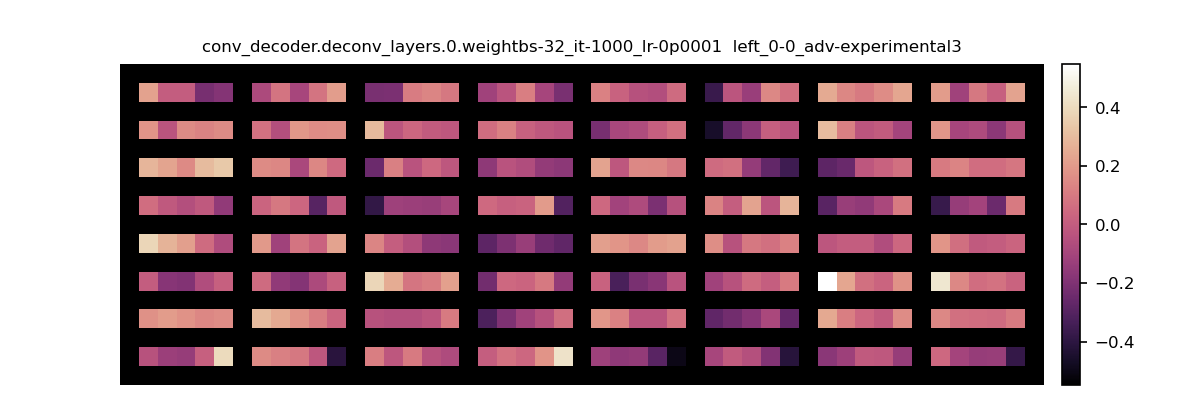
\includegraphics[width=0.3\textwidth]{./4_nn/figs/nn_adv_example_label_left_c1_dec}}
  \caption{Adversarial Training example of Generator (G) and Discriminator (D) of label \enquote{left} captured with 8 feature maps of the first convolutional layer.}
  \label{fig:nn_adv_example_label}
\end{figure}
\FloatBarrier
\noindent

Those trained weights from each label can then simply be put into the feature maps of a classification network.
This is shown in \rfig{nn_adv_example} where c1 from G and c2 from G in \rfig{nn_adv_example_label} were transfered to the first row(s).
When doing the transferring of feature maps, it is important that the layers are not mixed up so that the trained connections are still correct.
Also of course the weights of the feature maps must have the same dimension, so that transferring is possible.


\subsection{Observing the Generators output}
While the output of the Discriminator is rather uninteresting (one-dimensional probability value), the output of the Generator is a good indicator of how well the training between D and G has gone.
Optimally the output of the Generator look like real data samples.
An example of a trained Generator Network with fake outputs compared to real ones is shown in \rfig{nn_adv_gen}.

\begin{figure}[!ht]
  \centering
    \subfigure[\enquote{left} real examples]{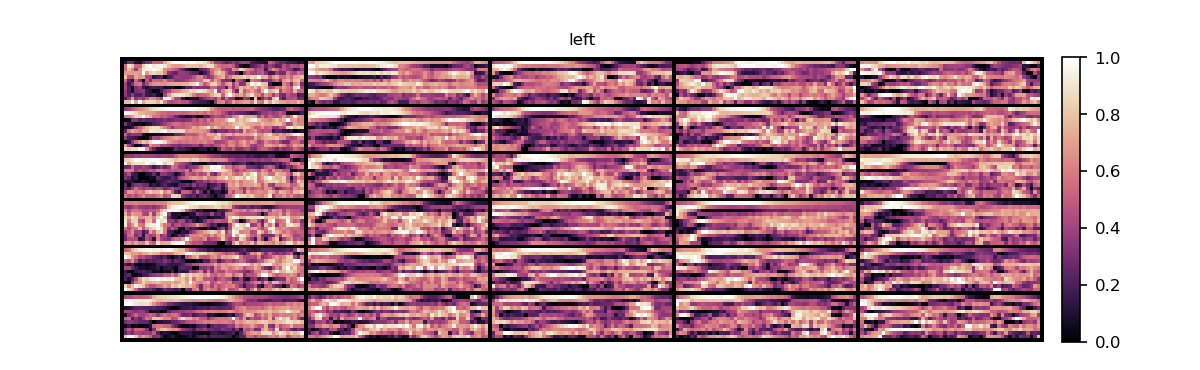
\includegraphics[width=0.45\textwidth]{./4_nn/figs/nn_adv_gen_left_real}}
    \subfigure[\enquote{left} fakes from G]{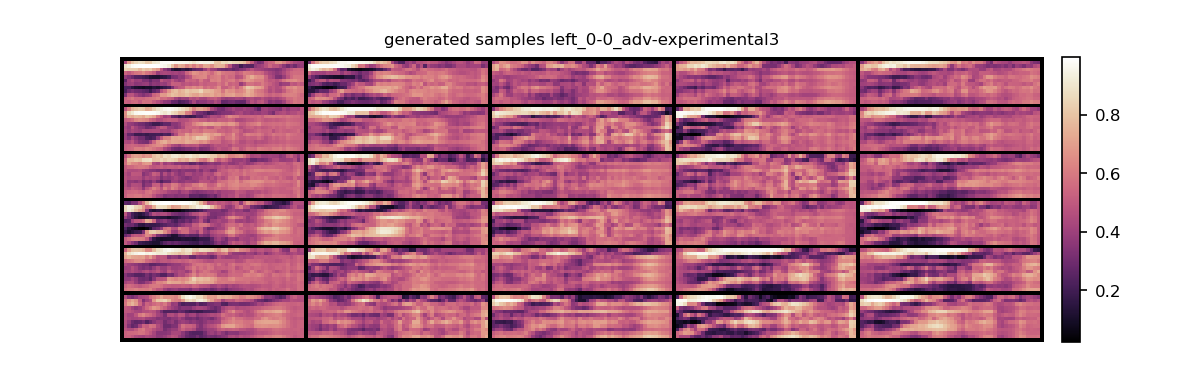
\includegraphics[width=0.45\textwidth]{./4_nn/figs/nn_adv_gen_left_fake}}
  \caption{Real samples of \enquote{left} from the Speech Commands dataset compared to fake samples from a trained Generator Network.}
  \label{fig:nn_adv_gen}
\end{figure}
\FloatBarrier
\noindent

If the fake example of the Generator Network do not look similar to real ones, then something might have gone wrong in the training between the Generator and Discriminator Network.
Further it can be evaluated if a certain network architecture is able to produce a label in a sufficient representation, therefore this method might be a good start in finding a suitable network architecture for the problem to be solved.




% --
% Experiments

\chapter{Experiments}\label{sec:exp}
All experiments hold within this thesis can be found in this chapter.
At the start it gives inside to the the Datasets and its feature extraction used for training the neural network architectures.
Some sound examples and their feature representation of the datasets are shown and the quality and diversity of recorded samples is mentioned.

More importantly this chapter includes the evaluation of the neural network models and their feature inputs in the application of speech command classification.
In Detail the feature selection is evaluated, to observe the impact of feature reduction.
Further the adversarial training approaches are compared to usual training.
Then the wavenet performances are shown...

% The training details are listed to give the reader an overview of the selected parameters for training, it should also give a shorten reference, so that not all parameters must be listed in the plots. 
% The training and evaluation consists of following evaluation tasks:
% \begin{enumerate}
%   \item Feature Selection
%   \item Adversarial Training
% \end{enumerate}

% dataset
% --
% dataset

\section{Dataset}\label{sec:exp_dataset}
Two datasets are used within this thesis, one is the second version of the speech commands dataset from \cite{Warden2018} and one is self made, denoted as \enquote{my dataset} which consists of only 5 labels that are especially valuable for movement in video games.

%(\enquote{left}, \enquote{right}, \enquote{right}, \enquote{right}).

Note that the \enquote{my dataset} is merely used for evaluation.
The training, validation and also testing of the neural network architectures is done on the speech commands dataset.
Both datasets consists of raw waveform files in the \texttt{.wav} format, no feature extraction was done beforehand.
As already mentioned in \rsec{prev_kws_benchmark} direct comparisons between different neural network approaches is a bit difficult if the feature extraction is left to the user alone.
Some datasets provide feature extraction beforehand, so that the comparability of neural network architectures performances is not influenced on it.
The speech commands dataset does no explicit separation into train, test and validation sets, but provides file lists that refers to distinct waveform files that should be used for test and validation.
More details of the datasets are presented below.


% Some abbreviations and references were done, so that the jungle of selected parameters get a little bit more clear to the reader of this thesis.
% The abbreviations of the dataset are shown in \rtab{exp_dataset_abbr}.

% The speech commands dataset is extracted before it is used for training. 
% To reduce computations in the evaluation process of neural networks, it was important to reduce the number of classes and examples per class to an suitable number.

% \begin{table}[ht!]
\begin{center}
\caption{Dataset abbreviations for label selection and feature group extraction.}
\begin{tabular}{ M{2cm} M{9cm} }
\toprule
%\multicolumn{4}{c}{\textbf{Feature Groups}} & \multicolumn{2}{c}{\textbf{Accuracy}} \\
\textbf{Abbreviation} & \textbf{Meaning}\\
\midrule
L5 & Selected labels: left, right, up, down, go\\
L10 & Selected labels: yes, no, left, go, down, off, right, stop, up, on\\
L30 & Selected labels: \enquote{all}\\
n[0-9]+ & Number of examples per class label, e.g. n500\\
\midrule
c[0-1] & Feature Group, use of cepstral features, 0 is false and 1 is true\\ 
d[0-1] & Feature Group, use of delta features, \ditto\\ 
dd[0-1] & Feature Group, use of double delta features, \ditto\\ 
e[0-1] & Feature Group, use of energy features, \ditto\\
norm[0-1] & features are normalized over frames\\
\bottomrule
\label{tab:exp_dataset_abbr}
\end{tabular}
\end{center}
\end{table}
\FloatBarrier
\noindent


% --
% speech commands dataset

\subsection{Speech Commands Dataset}\label{sec:exp_dataset_speech_cmd}
The speech command dataset \cite{Warden2018} consists of \SI{1}{\second} recordings from more than 30 different words, done by over thousands of different speakers.
The examples within the dataset were not recorded by professionals with high-end recording equipment, in fact their recording was done in an amateur kind of fashion, so that the dataset is more suited to realistic environments intended for user applications.
This is also noted in the paper \cite{Warden2018}:
\begin{quote}
...This meant that the use of studio-captured samples seemed unrealistic, since that audio would lack background noise, would be captured with high-quality microphones, and in a formal setting. 
Successful models would need to cope with noisy environments, poor quality recording equipment, and people talking in a natural, chatty way...
\end{quote}
The recording devices of the speakers, who contributed examples to the dataset, were in most cases simple consumer microphones, as for instance deployed in laptops or mobile phones.

The personal experiments made, when listening to the examples in the dataset, were:
\begin{itemize}
  \item The quality of the examples in the dataset are ranging from really good and understandable to very bad, noisy and unrecognizable, though most of the examples are good.

  \item Different accents can be perceived, that suggests that people from several countries were involved. However the bias is more on American English as noted in the paper.

  \item No children speakers were found on the personal listening.
\end{itemize}

Due to data privacy issues the information on the individual speakers are not given.
Further it is not clear if there are equal amounts of male and female speakers and if there are any children speakers included.
The last would be especially interesting for a video games suited for kids.

In many recordings the background noise is imminent, such as traffic noise, chattering people, office sounds, etc.
Some quality check of the recorded files in the dataset was done by the author of \cite{Warden2018} to reject bad samples.
However there are still some existing flaws such as too loud or too silent files or examples with inconsistent sample numbers or some examples that are prone with too much noise or in the worst case, noise only.
Those quality issues in the dataset are for most cases neglectable or can be fixed, such as inconsistent sample numbers. 
Other more problematic cases, for instance noise-only examples, should be filtered out.
%Still it is a great dataset, because there is no need for a perfect dataset when working with neural networks and one can be happy that there exists one with this amount of diversity and free of access under the creative common license.
Usually its not a problem for neural networks to cope with unclean datasets, because of their ability to learn invariance against noise, loudness differences and other nuisances during training.
Further if the training dataset is large enough and the test and validation sets do not include really bad examples, then there should be no big issues.
However some cleanu up of the dataset was still done as described in...

The speech command dataset exists in two versions (\texttt{v0.01} and \texttt{v0.02}), the first one was published in 2017 and the second one emerged as improved version of \texttt{v0.01} with more key words, examples and quality in 2018.
In this thesis, the experiments are done on the second version \texttt{v0.02}.

Some examples of the speech command dataset in raw audio format are shown in \rfig{exp_dataset_wav_grid_c30} and give a small glimpse on the quality of the recordings.
\begin{figure}[!ht]
  \centering
    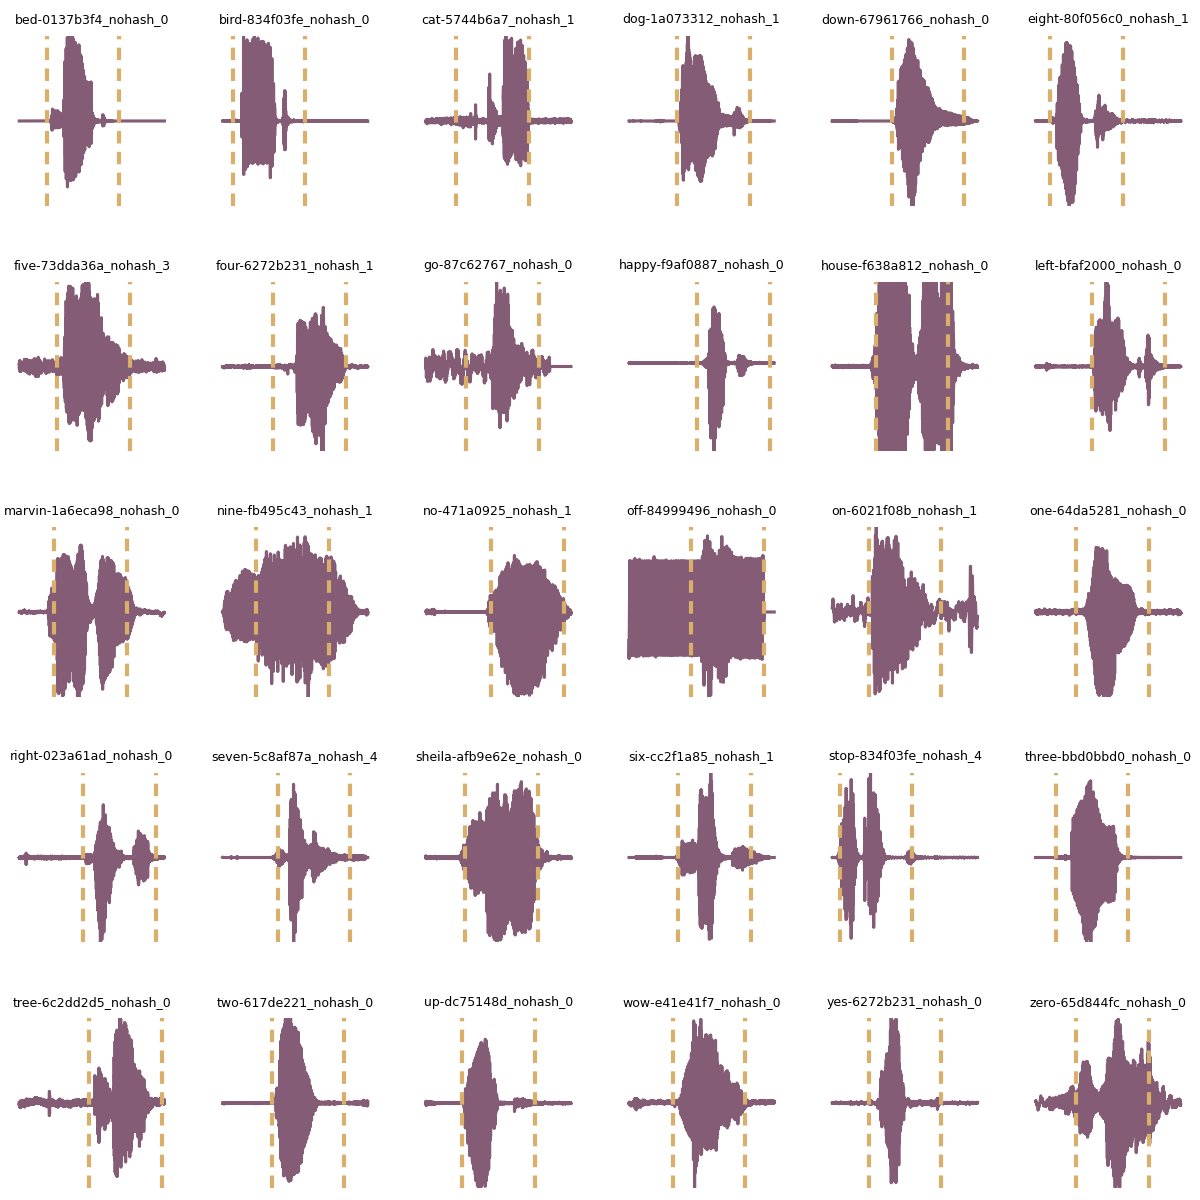
\includegraphics[width=0.65\textwidth]{./5_exp/figs/exp_dataset_wav_grid_c30}
  \caption{One random sample of each individual speech command in the speech command dataset in normalized raw audio format.}
  \label{fig:exp_dataset_wav_grid_c30}
\end{figure}
\FloatBarrier
\noindent

% dataset structure
\subsubsection{Dataset Structure}
The speech command examples are stored in separate folders, named after each individual speech command, in the \texttt{.wav} format.
The folder named as \texttt{\_background\_noise\_} contains six different background noise files, such as \texttt{white\_noise.wav} or \texttt{doing\_the\_dishes.wav}, with a duration of more than one minute each.
Noise examples with a new noise label named \texttt{_noise} were extracted from those background noise files with a \SI{1}{\second} window shifted by \SI{0.2}{\second}.

Each waveform file is named with an 8-digit hexadecimal hash code for the speaker identification, followed by the utterance number, for instance \texttt{3b4f8f24\_nohash\_0.wav}.
Therefore it is possible to distinguish between different speakers, however as mentioned above, no further information about the speaker is given due to data privacy issues.

%It has to be mentioned, that it is wonderful, that a dataset for simple key word spotting on speech commands with this amount of diversity and free of access under the creative common license exist.


% --
% my dataset

\subsection{My own Dataset}\label{sec:exp_dataset_my}
This dataset was created by the author of this thesis and contains five examples samples each from the words \{\enquote{left}, \enquote{right}, \enquote{up}, \enquote{down} and \enquote{go}\}.
The datasets purpose is mainly to have an additional test set for evaluating trained models on the authors own voice with different word pronouncement on each example.
It is important to mention that none of the self recorded files were used within the training set, so that the neural networks performance on this unseen data is evaluated.
All examples of my own dataset are illustrated in \rfig{exp_dataset_wav_grid_my} in raw audio format.
\begin{figure}[!ht]
  \centering
    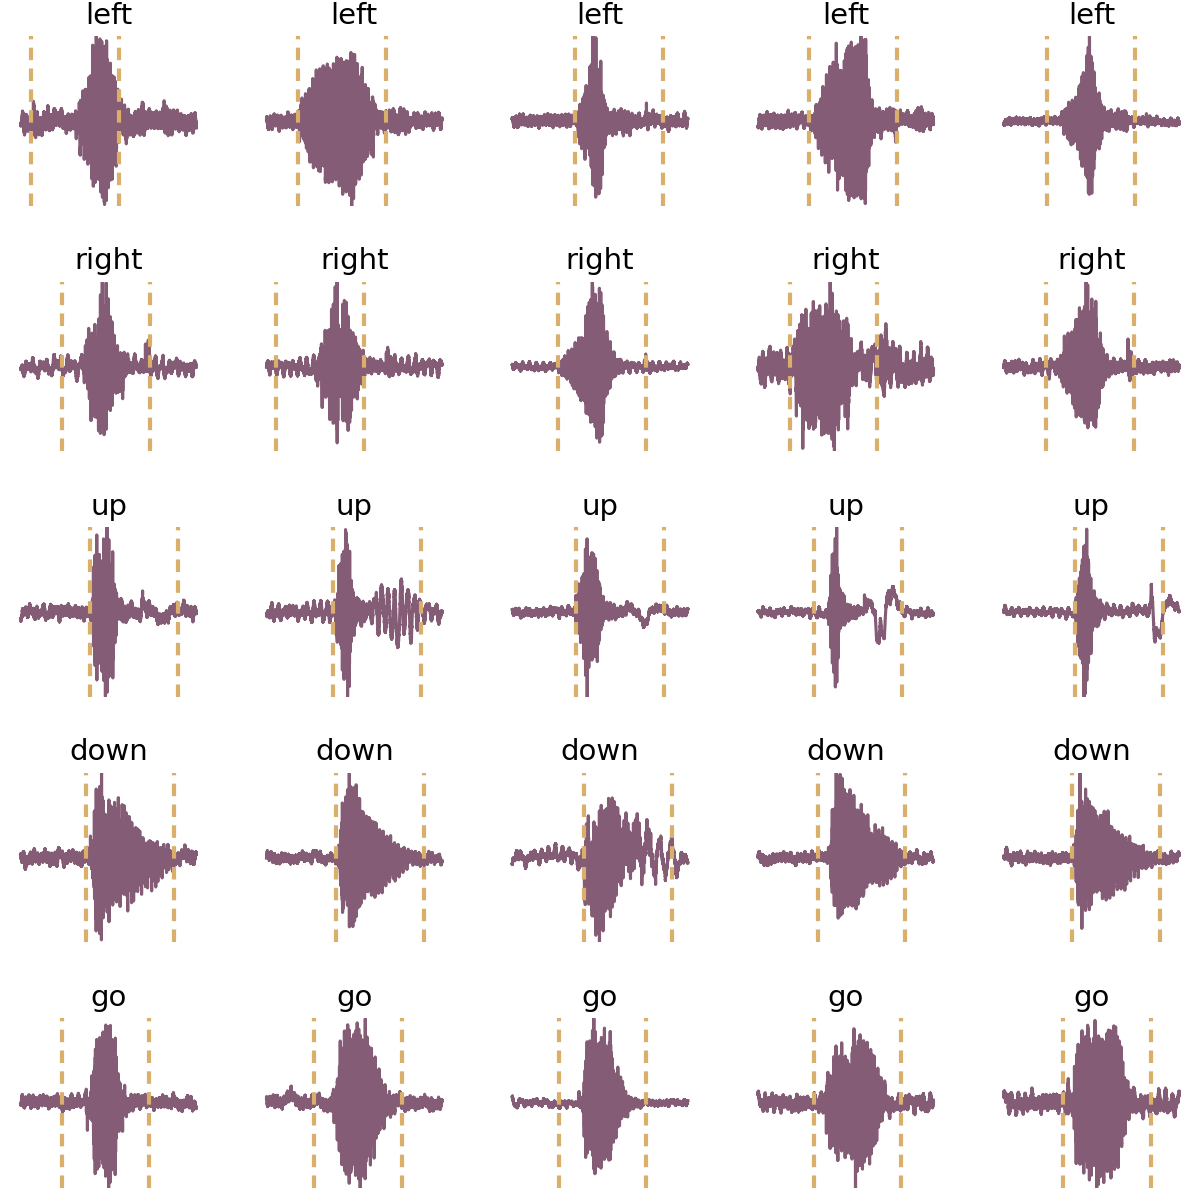
\includegraphics[width=0.65\textwidth]{./5_exp/figs/exp_dataset_wav_grid_my}
  \caption{Self recorded files of the \enquote{my dataset} in raw audio format.}
  \label{fig:exp_dataset_wav_grid_my}
\end{figure}
\FloatBarrier
\noindent
The examples per word are spoken with different emphasis and stress on individual phonemes.
Also the prolongation of the words are different, that in one example the word is fast and in the other its slow spoken.
The emphasis and prolongation ensure the diversity of the dataset. 
It turned out that it is not easy for neural networks to gain a $100\%$ classification score upon it, even though there is only one and the same speaker.


% --
% Speech Commands dataset

\subsection{Speech Commands Dataset}\label{sec:exp_dataset_speech_cmd}
The speech command dataset \cite{Warden2018} is a very diverse dataset consisting of over thousands of different speakers. 
This dataset is by any means no clean dataset recorded by professionals, if anything it is the opposite and therefore more suitable to realistic environments, as noted in the paper:
\begin{quote}
...I made the decision to focus on capturing audio that reflected the on-device trigger phrase task described above. 
This meant that the use of studio-captured samples seemed unrealistic, since that audio would lack background noise, would be captured with high-quality microphones, and in a formal setting...
\end{quote}
The recording devices of the speakers were simply the next microphones they could grab, such as in laptops or mobile phones.
In many recordings the background noise is imminent, such as traffic, chattering people, office sounds, etc.
Some quality check of the recorded files has been done to reject bad samples.
However there are still some existing flaws such as too loud or too silent files or examples with inconsistent sample numbers and some examples are prone with too much noise or in the worst case, noise only.
Those quality issues in the dataset are for most cases neglectable or can be fixed, such as inconsistent sample numbers, other more problematic cases, for instance noise only examples, should be filtered out.
%Still it is a great dataset, because there is no need for a perfect dataset when working with neural networks and one can be happy that there exists one with this amount of diversity and free of access under the creative common license.
Maybe its even better to have an unclean dataset, so that invariance against noise and loudness are learnt during training.

Some examples of the speech command dataset in raw audio format are shown in \rfig{exp_dataset_wav_grid_c30} and give a small inside on the quality of the recordings.
\begin{figure}[!ht]
  \centering
    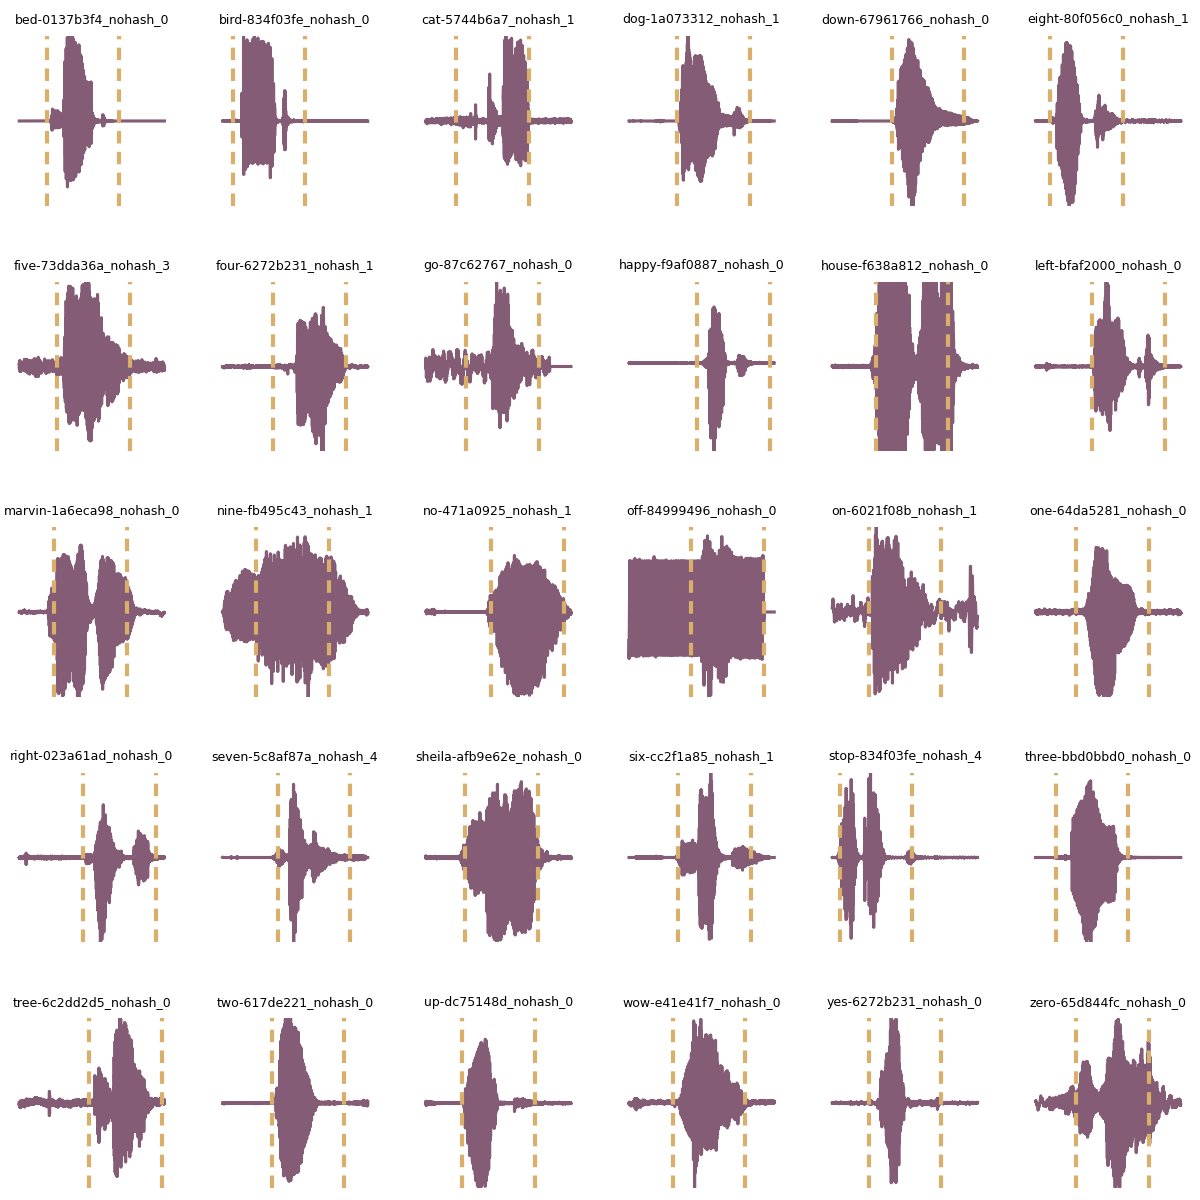
\includegraphics[width=0.65\textwidth]{./5_exp/figs/exp_dataset_wav_grid_c30}
  \caption{One random sample of each individual speech command in the speech command dataset in normalized raw audio format.}
  \label{fig:exp_dataset_wav_grid_c30}
\end{figure}
\FloatBarrier
\noindent

%It has to be mentioned, that it is wonderful, that a dataset for simple key word spotting on speech commands with this amount of diversity and free of access under the creative common license exist.


% --
% my dataset

\subsection{My own Dataset}\label{sec:exp_dataset_my}
This dataset is created by the author of this thesis and contain 5 speech command samples from the words (classes) \enquote{left}, \enquote{right}, \enquote{up}, \enquote{down} and \enquote{go}.
Its purpose is mainly as test set in evaluating trained models.
It is important to mention that none of the self recorded files are used within the training set, so that it the neural networks performance on unseen data is evaluated.
All examples of my own dataset are illustrated in \rfig{exp_dataset_wav_grid_my} in raw audio format.
\begin{figure}[!ht]
  \centering
    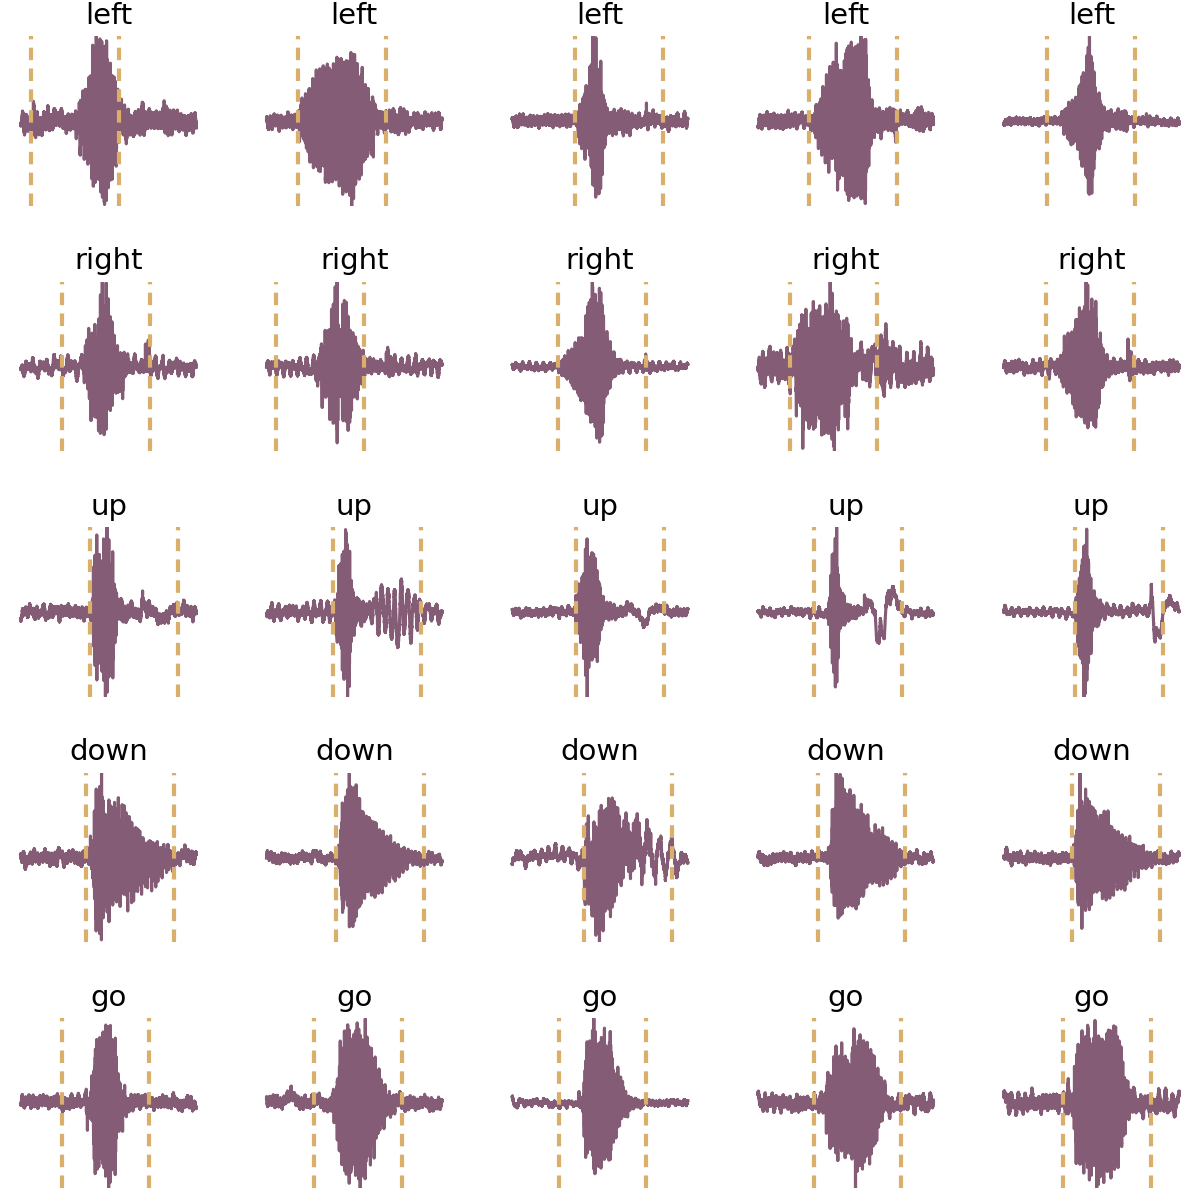
\includegraphics[width=0.65\textwidth]{./5_exp/figs/exp_dataset_wav_grid_my}
  \caption{Self recorded files of the \enquote{my dataset} in raw audio format.}
  \label{fig:exp_dataset_wav_grid_my}
\end{figure}
\FloatBarrier
\noindent
The examples per class are spoken with different emphasis and stress on individual phonemes, such that they do not sound the same.
Also the prolongation of the words are different, such that in one example the word is fast and in the other its slow spoken.
The emphasis and prolongation ensure the diversity of the dataset and it turned out that it is not easy for neural networks to gain a $100\%$ classification rate upon it, even though there is only one and the same speaker.


% neural networks
% --
% training details

\section{Implementation and Training Details}\label{sec:exp_details}
In this sections, the implementation und parameters for training are is described in more detail.

\subsection{Implementation notes}\label{sec:exp_details_implementation}
The programming code for this thesis was entirely done in \texttt{Python} with version $>3.8$ evaluated on a linux system.
This might be important if one tries to run the python code on a windows machine, it was not tested for it and could yield in errors (especially regarding paths variables).
For the neural networks implementation and training, the framework \texttt{Pytorch} with version $1.7.0$ was used. 
Usually it should not be a problem if a newer version of \texttt{Pytorch} is applied.
The feature extraction with Mel Frequency Cepstral Coefficients (MFCC) was done with an own implementation, but using efficients functions for transforms functions, such as the short time fourier transform, with packages from \texttt{scipy}.
Matrix computations usually are done with the package \texttt{numpy}.
Several other \texttt{Python} packages were used within the project, but are not named explicitly.


\subsection{Neural Network Training Details}\label{sec:exp_details_training}
We can separate the training details into following parameters to select from:
\begin{enumerate}
  \item Features extraction parameters
  \item Dataset parameters
  \item Feature selection
  \item Transfer Learning parameters
  \item Machine Learning parameters
\end{enumerate}
The feature extraction parameters simply give information about how features are extracted, e.g. this includes the hop size, frame size, filter bands of the MFCC, etc.
The dataset parameters are the information of which labels and how many examples per labels are used
Also they consist of the feature selection, so that the extracted dataset only consists of MFCC data. 
The Abbreviation regarding dataset parameters and feature selection were already listed in \rtab{exp_dataset_abbr}.
%The feature selection is the information about what input feature groups are used in the training, e.g. use cepstral coefficients only, or add delta and energy features, their references are shown in \rtab{dataset_feature_groups}.
The Transfer Learning parameters are pre-trained weights for the actual neural network architecture to be trained.
This could be only the first convolutional layers or entire networks but here all convolutional layers from an adversarial training are considered. 
The Abbreviations for training parameters can be specified as listed in \rtab{exp_details_adv}
\begin{table}[ht!]
\begin{center}
\caption{Adversarial Training abbreviations.}
\begin{tabular}{ M{2cm}  M{5cm} }
\toprule
%\multicolumn{4}{c}{\textbf{Feature Groups}} & \multicolumn{2}{c}{\textbf{Accuracy}} \\
\textbf{Abbreviations} & \textbf{Meaning}\\
\midrule
dec & use of decoder weights\\
enc & use of encoder weights\\
itl[0-9]+ & iterations per label, e.g. itl500 for 500 iterations\\
\bottomrule
\label{tab:exp_details_adv}
\end{tabular}
\end{center}
\end{table}
\FloatBarrier
\noindent


The Machine Learning parameters are classically training parameters such as learning rate, number of epochs, etc.
Their selection and references are listed in \rtab{exp_details_train_params}

\begin{table}[ht!]
\begin{center}
\caption{All training parameters used within this thesis and their abbreviations.}
\begin{tabular}{ M{2cm}  M{5cm} }
\toprule
%\multicolumn{4}{c}{\textbf{Feature Groups}} & \multicolumn{2}{c}{\textbf{Accuracy}} \\
\textbf{Abbreviations} & \textbf{Meaning}\\
\midrule
it[0-9]+ & Number of epochs (or iterations)\\
bs[0-9]+ & Batch size, e.g. bs32 is a batch size of 32 examples\\
lr[0-9.]+ & Learning rate, e.g. lr0.0001\\
mo[0-9.]+ & Momentum, e.g. mo0.5\\
\bottomrule
\label{tab:exp_details_train_params}
\end{tabular}
\end{center}
\end{table}
\FloatBarrier
\noindent


% --
% feature selection

\section{Feature Selection}\label{sec:exp_fs}
The first important Question, when using Neural Networks, is what features are used as inputs.
In the feature extraction section about MFCCs \rsec{signal_mfcc}, it was shown how raw audio files can be extracted to MFCCs and what enhancements can be done.
These enhancements (deltas and energy features) are formed in groups for evaluation to see the impact on the choice and hopefully to reduce the input feature size to a minimum.
%Now that the Neural Network Architectures are described in \rsec{nn_arch} and basic knowledge about MFCCs is given in \rsec{features} it is important to evaluate the impact of the selection of certain MFCC feature constellations to the accuracy of the Test sets.
Beside it is good to get a general overview on what accuracies can be expected from different Neural Network Architectures.
The evaluation is done on 5 classes and 30 classes with different training parameters to observe the impact on a easy and a very hard classification task.
In detail it is shown how models are trained with features consisting of following MFCC groups:
\begin{enumerate}
    \item Cepstral Coefficients (usual MFCCs)
    \item Deltas (frame difference of MFCCs)
    \item Double Deltas (frame difference of Deltas)
    \item Energy Vector (added to each of the upper features)
\end{enumerate}
Another crucial point is to evaluate whether a frame based normalization of these features hurt the training and the accuracy of the models.
Therefore additional columns are presented in the following tables marked with \enquote{norm}.
Note that all these experiments have been done with n-500 a number of 500 examples per class, so that computations are minimized but still enough data is drawn.

\subsection{Feature Selection on Conv Encoder}
The feature selection evaluation on the conv-encoder-fc1 architecture with 5 labels is listed in \rtab{exp_fs_fc1_it500_c5}.
% \begin{table}[ht!]
\begin{center}
\caption{Feature Selection ml it500 c5 features fc1}
\begin{tabular}{ M{1cm}  M{1cm}  M{1cm}  M{1cm}  M{1.5cm}  M{1.5cm}  M{1.5cm}  M{1.5cm} }
\toprule
\multicolumn{4}{c}{\textbf{Feature Groups}} & \multicolumn{2}{c}{\textbf{Accuracy}} \\
\textbf{c} & \textbf{d} & \textbf{dd} & \textbf{e} & \textbf{acc test} & \textbf{acc my} & \textbf{acc test norm} & \textbf{acc my norm} \\
\midrule
0 & 0 & 1 & 0 & 86.67 & 80.00 & 68.33 & 73.33 \\
0 & 0 & 1 & 1 & 85.00 & 86.67 & 67.67 & 73.33 \\
0 & 1 & 0 & 0 & 92.67 & 100.00 & 75.67 & 80.00 \\
0 & 1 & 0 & 1 & 90.67 & 90.00 & 82.00 & 73.33 \\
0 & 1 & 1 & 0 & 91.00 & 93.33 & 76.67 & 70.00 \\
0 & 1 & 1 & 1 & 89.33 & 100.00 & 78.67 & 80.00 \\
1 & 0 & 0 & 0 & 16.67 & 16.67 & 88.33 & 86.67 \\
1 & 0 & 0 & 1 & 33.33 & 33.33 & 86.33 & 80.00 \\
1 & 0 & 1 & 0 & 91.00 & 90.00 & 87.00 & 80.00 \\
1 & 0 & 1 & 1 & 82.67 & 86.67 & 86.67 & 90.00 \\
1 & 1 & 0 & 0 & 91.67 & 76.67 & 88.33 & 90.00 \\
1 & 1 & 0 & 1 & 90.00 & 80.00 & 89.33 & 93.33 \\
1 & 1 & 1 & 0 & 89.00 & 76.67 & 89.33 & 90.00 \\
1 & 1 & 1 & 1 & 88.00 & 90.00 & 89.00 & 86.67 \\
\bottomrule
\end{tabular}
\end{center}
\label{tab:ml_it500_c5_features_fc1}
\end{table}
\FloatBarrier
\noindent


% \begin{table}[ht!]
\begin{center}
\caption{Feature Selection ml it1000 c30 features fc1}
\begin{tabular}{ M{1cm}  M{1cm}  M{1cm}  M{1cm}  M{1.5cm}  M{1.5cm} }
\toprule
\multicolumn{4}{c}{\textbf{Feature Groups}} & \multicolumn{2}{c}{\textbf{Accuracy}} \\
\textbf{c} & \textbf{d} & \textbf{dd} & \textbf{e} & \textbf{acc test} & \textbf{acc test norm} \\
\midrule
0 & 0 & 1 & 0 & 52.97 & 33.10 \\
0 & 0 & 1 & 1 & 56.65 & 27.94 \\
0 & 1 & 0 & 0 & 63.55 & 39.68 \\
0 & 1 & 0 & 1 & 74.52 & 48.65 \\
0 & 1 & 1 & 0 & 71.03 & 39.35 \\
0 & 1 & 1 & 1 & 73.94 & 46.39 \\
1 & 0 & 0 & 0 & 47.23 & 58.19 \\
1 & 0 & 0 & 1 & 45.35 & 57.81 \\
1 & 0 & 1 & 0 & 60.45 & 47.55 \\
1 & 0 & 1 & 1 & 59.48 & 51.61 \\
1 & 1 & 0 & 0 & 58.77 & 55.10 \\
1 & 1 & 0 & 1 & 6.45 & 47.81 \\
1 & 1 & 1 & 0 & 65.81 & 60.39 \\
1 & 1 & 1 & 1 & 62.06 & 51.55 \\
\bottomrule
\end{tabular}
\end{center}
\label{tab:ml_it1000_c30_features_fc1}
\end{table}
\FloatBarrier
\noindent


% \begin{table}[ht!]
\begin{center}
\caption{Feature Selection ml it2000 c30 features fc3}
\begin{tabular}{ M{1cm}  M{1cm}  M{1cm}  M{1cm}  M{1.5cm}  M{1.5cm} }
\toprule
\multicolumn{4}{c}{\textbf{Feature Groups}} & \multicolumn{2}{c}{\textbf{Accuracy}} \\
\textbf{c} & \textbf{d} & \textbf{dd} & \textbf{e} & \textbf{acc test} & \textbf{acc test norm} \\
\midrule
0 & 0 & 1 & 0 & 49.03 & 33.74 \\
0 & 0 & 1 & 1 & 66.90 & 34.84 \\
0 & 1 & 0 & 0 & 77.10 & 55.55 \\
0 & 1 & 0 & 1 & 78.65 & 56.52 \\
0 & 1 & 1 & 0 & 74.97 & 50.26 \\
0 & 1 & 1 & 1 & 73.94 & 59.61 \\
1 & 0 & 0 & 0 & 76.52 & 64.26 \\
1 & 0 & 0 & 1 & 73.87 & 59.16 \\
1 & 0 & 1 & 0 & 78.58 & 63.03 \\
1 & 0 & 1 & 1 & 73.48 & 59.03 \\
1 & 1 & 0 & 0 & 79.10 & 66.13 \\
1 & 1 & 0 & 1 & 80.39 & 60.77 \\
1 & 1 & 1 & 0 & 76.97 & 64.71 \\
1 & 1 & 1 & 1 & 75.94 & 65.55 \\
\bottomrule
\end{tabular}
\end{center}
\label{tab:ml_it2000_c30_features_fc3}
\end{table}
\FloatBarrier
\noindent


\begin{table}[ht!]
\begin{center}
\caption{Feature Selection on arch: conv-encoder-fc1 with dataset: L5-n500 and training params: it500-bs32-lr0.0001-mo0.5}
\begin{tabular}{ M{1cm}  M{1cm}  M{1cm}  M{1cm}  M{1.5cm}  M{1.5cm}  M{1.5cm}  M{1.5cm} }
\toprule
\multicolumn{4}{c}{\textbf{Feature Groups}} & \multicolumn{2}{c}{\textbf{Accuracy}} \\
\textbf{c} & \textbf{d} & \textbf{dd} & \textbf{e} & \textbf{acc test} & \textbf{acc my} & \textbf{acc test norm} & \textbf{acc my norm} \\
\midrule
0 & 0 & 1 & 0 & 86.67 & 80.00 & 68.33 & 73.33 \\
0 & 0 & 1 & 1 & 85.00 & 86.67 & 67.67 & 73.33 \\
0 & 1 & 0 & 0 & 92.67 & 100.00 & 75.67 & 80.00 \\
0 & 1 & 0 & 1 & 90.67 & 90.00 & 82.00 & 73.33 \\
0 & 1 & 1 & 0 & 91.00 & 93.33 & 76.67 & 70.00 \\
0 & 1 & 1 & 1 & 89.33 & 100.00 & 78.67 & 80.00 \\
1 & 0 & 0 & 0 & 16.67 & 16.67 & 88.33 & 86.67 \\
1 & 0 & 0 & 1 & 33.33 & 33.33 & 86.33 & 80.00 \\
1 & 0 & 1 & 0 & 91.00 & 90.00 & 87.00 & 80.00 \\
1 & 0 & 1 & 1 & 82.67 & 86.67 & 86.67 & 90.00 \\
1 & 1 & 0 & 0 & 91.67 & 76.67 & 88.33 & 90.00 \\
1 & 1 & 0 & 1 & 90.00 & 80.00 & 89.33 & 93.33 \\
1 & 1 & 1 & 0 & 89.00 & 76.67 & 89.33 & 90.00 \\
1 & 1 & 1 & 1 & 88.00 & 90.00 & 89.00 & 86.67 \\
\bottomrule
\label{tab:exp_fs_fc1_it500_c5}
\end{tabular}
\end{center}
\end{table}
\FloatBarrier
\noindent


\begin{table}[ht!]
\begin{center}
\caption{Feature Selection on arch: conv-encoder-fc1 with dataset: L30-n500 and training params: it1000-bs128-lr0.0001-mo0.5}
\begin{tabular}{ M{1cm}  M{1cm}  M{1cm}  M{1cm}  M{1.5cm}  M{1.5cm} }
\toprule
\multicolumn{4}{c}{\textbf{Feature Groups}} & \multicolumn{2}{c}{\textbf{Accuracy}} \\
\textbf{c} & \textbf{d} & \textbf{dd} & \textbf{e} & \textbf{acc test} & \textbf{acc test norm} \\
\midrule
0 & 0 & 1 & 0 & 52.97 & 33.10 \\
0 & 0 & 1 & 1 & 56.65 & 27.94 \\
0 & 1 & 0 & 0 & 63.55 & 39.68 \\
0 & 1 & 0 & 1 & 74.52 & 48.65 \\
0 & 1 & 1 & 0 & 71.03 & 39.35 \\
0 & 1 & 1 & 1 & 73.94 & 46.39 \\
1 & 0 & 0 & 0 & 47.23 & 58.19 \\
1 & 0 & 0 & 1 & 45.35 & 57.81 \\
1 & 0 & 1 & 0 & 60.45 & 47.55 \\
1 & 0 & 1 & 1 & 59.48 & 51.61 \\
1 & 1 & 0 & 0 & 58.77 & 55.10 \\
1 & 1 & 0 & 1 & 6.45 & 47.81 \\
1 & 1 & 1 & 0 & 65.81 & 60.39 \\
1 & 1 & 1 & 1 & 62.06 & 51.55 \\
\bottomrule
\label{tab:exp_fs_fc1_it1000_c30}
\end{tabular}
\end{center}
\end{table}
\FloatBarrier
\noindent


\begin{table}[ht!]
\begin{center}
\caption{Feature Selection on arch: conv-encoder-fc3 with dataset: L30-n500 and training params: it2000-bs128-lr0.0001-mo0.5}
\begin{tabular}{ M{1cm}  M{1cm}  M{1cm}  M{1cm}  M{1.5cm}  M{1.5cm} }
\toprule
\multicolumn{4}{c}{\textbf{Feature Groups}} & \multicolumn{2}{c}{\textbf{Accuracy}} \\
\textbf{c} & \textbf{d} & \textbf{dd} & \textbf{e} & \textbf{acc test} & \textbf{acc test norm} \\
\midrule
0 & 0 & 1 & 0 & 49.03 & 33.74 \\
0 & 0 & 1 & 1 & 66.90 & 34.84 \\
0 & 1 & 0 & 0 & 77.10 & 55.55 \\
0 & 1 & 0 & 1 & 78.65 & 56.52 \\
0 & 1 & 1 & 0 & 74.97 & 50.26 \\
0 & 1 & 1 & 1 & 73.94 & 59.61 \\
1 & 0 & 0 & 0 & 76.52 & 64.26 \\
1 & 0 & 0 & 1 & 73.87 & 59.16 \\
1 & 0 & 1 & 0 & 78.58 & 63.03 \\
1 & 0 & 1 & 1 & 73.48 & 59.03 \\
1 & 1 & 0 & 0 & 79.10 & 66.13 \\
1 & 1 & 0 & 1 & 80.39 & 60.77 \\
1 & 1 & 1 & 0 & 76.97 & 64.71 \\
1 & 1 & 1 & 1 & 75.94 & 65.55 \\
\bottomrule
\label{tab:exp_fs_fc3_it2000_c30}
\end{tabular}
\end{center}
\end{table}
\FloatBarrier
\noindent



\subsection{Feature Selection on fstride}
fstride
\begin{table}[ht!]
\begin{center}
\caption{Feature Selection on arch: conv-fstride with dataset: L5-n500 and training params: it1000-bs32-lr0.0001-mo0.5}
\begin{tabular}{ M{1cm}  M{1cm}  M{1cm}  M{1cm}  M{1.5cm}  M{1.5cm}  M{1.5cm}  M{1.5cm} }
\toprule
\multicolumn{4}{c}{\textbf{Feature Groups}} & \multicolumn{2}{c}{\textbf{Accuracy}} \\
\textbf{c} & \textbf{d} & \textbf{dd} & \textbf{e} & \textbf{acc test} & \textbf{acc my} & \textbf{acc test norm} & \textbf{acc my norm} \\
\midrule
0 & 0 & 1 & 0 & 65.67 & 56.67 & 43.67 & 53.33 \\
0 & 0 & 1 & 1 & 64.33 & 60.00 & 49.00 & 43.33 \\
0 & 1 & 0 & 0 & 86.00 & 83.33 & 69.00 & 63.33 \\
0 & 1 & 0 & 1 & 85.00 & 76.67 & 67.67 & 83.33 \\
0 & 1 & 1 & 0 & 84.67 & 76.67 & 72.33 & 73.33 \\
0 & 1 & 1 & 1 & 84.00 & 80.00 & 76.00 & 66.67 \\
1 & 0 & 0 & 0 & 88.33 & 76.67 & 84.33 & 73.33 \\
1 & 0 & 0 & 1 & 90.00 & 86.67 & 81.67 & 70.00 \\
1 & 0 & 1 & 0 & 89.00 & 80.00 & 86.00 & 86.67 \\
1 & 0 & 1 & 1 & 88.67 & 83.33 & 83.67 & 80.00 \\
1 & 1 & 0 & 0 & 89.33 & 83.33 & 86.33 & 73.33 \\
1 & 1 & 0 & 1 & 90.00 & 80.00 & 86.67 & 80.00 \\
1 & 1 & 1 & 0 & 89.00 & 76.67 & 86.33 & 73.33 \\
1 & 1 & 1 & 1 & 90.67 & 86.67 & 86.00 & 86.67 \\
\bottomrule
\label{tab:exp_fs_fstride_it1000_c5}
\end{tabular}
\end{center}
\end{table}
\FloatBarrier
\noindent



\subsection{Feature Selection on trad}
trad
\begin{table}[ht!]
\begin{center}
\caption{Feature Selection on arch: conv-trad with dataset: L5-n500 and training params: it1000-bs32-lr0.0001-mo0.5}
\begin{tabular}{ M{1cm}  M{1cm}  M{1cm}  M{1cm}  M{1.5cm}  M{1.5cm}  M{1.5cm}  M{1.5cm} }
\toprule
\multicolumn{4}{c}{\textbf{Feature Groups}} & \multicolumn{2}{c}{\textbf{Accuracy}} \\
\textbf{c} & \textbf{d} & \textbf{dd} & \textbf{e} & \textbf{acc test} & \textbf{acc my} & \textbf{acc test norm} & \textbf{acc my norm} \\
\midrule
0 & 0 & 1 & 0 & 84.00 & 86.67 & 65.33 & 56.67 \\
0 & 0 & 1 & 1 & 85.67 & 86.67 & 72.00 & 66.67 \\
0 & 1 & 0 & 0 & 91.67 & 83.33 & 84.67 & 66.67 \\
0 & 1 & 0 & 1 & 93.33 & 93.33 & 83.33 & 80.00 \\
0 & 1 & 1 & 0 & 93.33 & 86.67 & 86.33 & 80.00 \\
0 & 1 & 1 & 1 & 91.67 & 90.00 & 90.33 & 80.00 \\
1 & 0 & 0 & 0 & 94.33 & 93.33 & 92.00 & 83.33 \\
1 & 0 & 0 & 1 & 95.00 & 90.00 & 91.00 & 93.33 \\
1 & 0 & 1 & 0 & 93.67 & 90.00 & 94.67 & 83.33 \\
1 & 0 & 1 & 1 & 91.67 & 96.67 & 94.00 & 76.67 \\
1 & 1 & 0 & 0 & 95.00 & 83.33 & 92.67 & 83.33 \\
1 & 1 & 0 & 1 & 94.67 & 93.33 & 92.00 & 86.67 \\
1 & 1 & 1 & 0 & 95.33 & 90.00 & 92.00 & 86.67 \\
1 & 1 & 1 & 1 & 95.00 & 100.00 & 94.00 & 86.67 \\
\bottomrule
\label{tab:exp_fs_trad_it1000_c5}
\end{tabular}
\end{center}
\end{table}
\FloatBarrier
\noindent




% --
% adversarial training

\section{Adversarial Training}\label{sec:exp_adv}
\thesisStateNotReady
Here the Adversarial Training is evalutated.
The first comparance is between a the conv-encoder-fc3 once with adversarial init (use of) and once with simple random init.
The training losses of those two methods are shown in \rfig{exp_adv_fc3_train_loss} and their accuracies in \rfig{exp_adv_fc3_val_acc}.

\begin{figure}[!ht]
  \centering
    \subfigure[adv init]{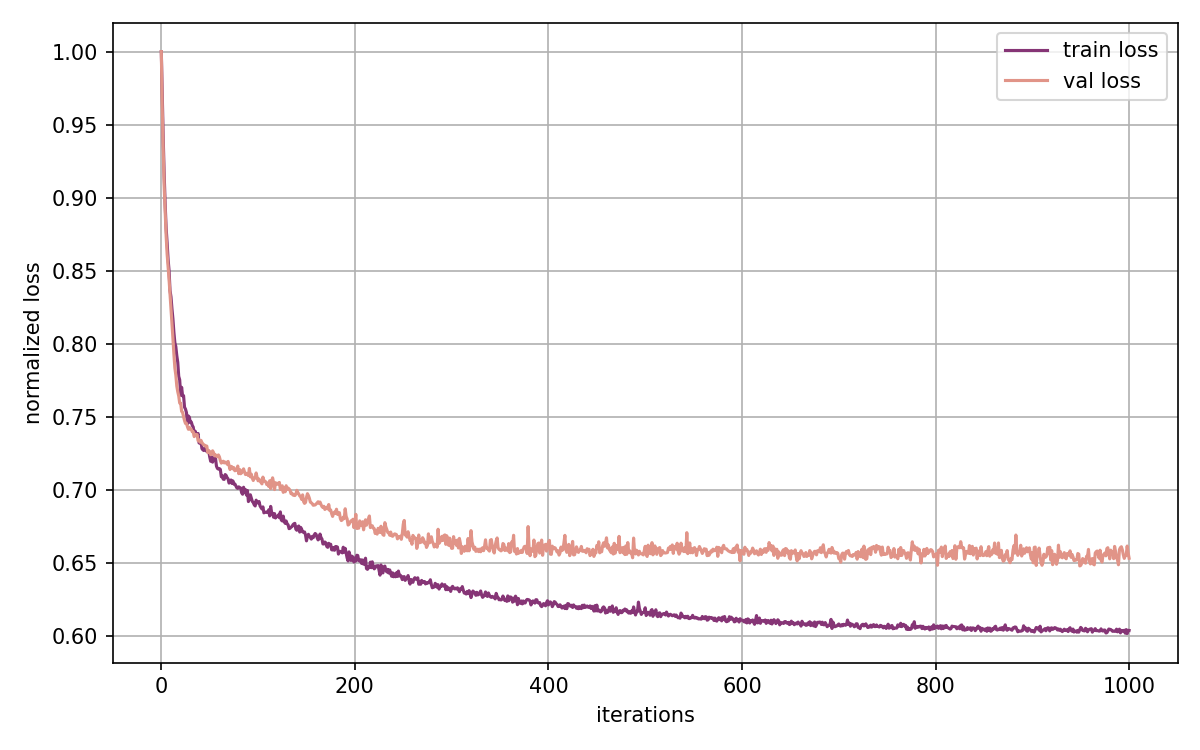
\includegraphics[width=0.45\textwidth]{./5_exp/figs/exp_adv_fc3_train_loss_label}}
    \subfigure[random init]{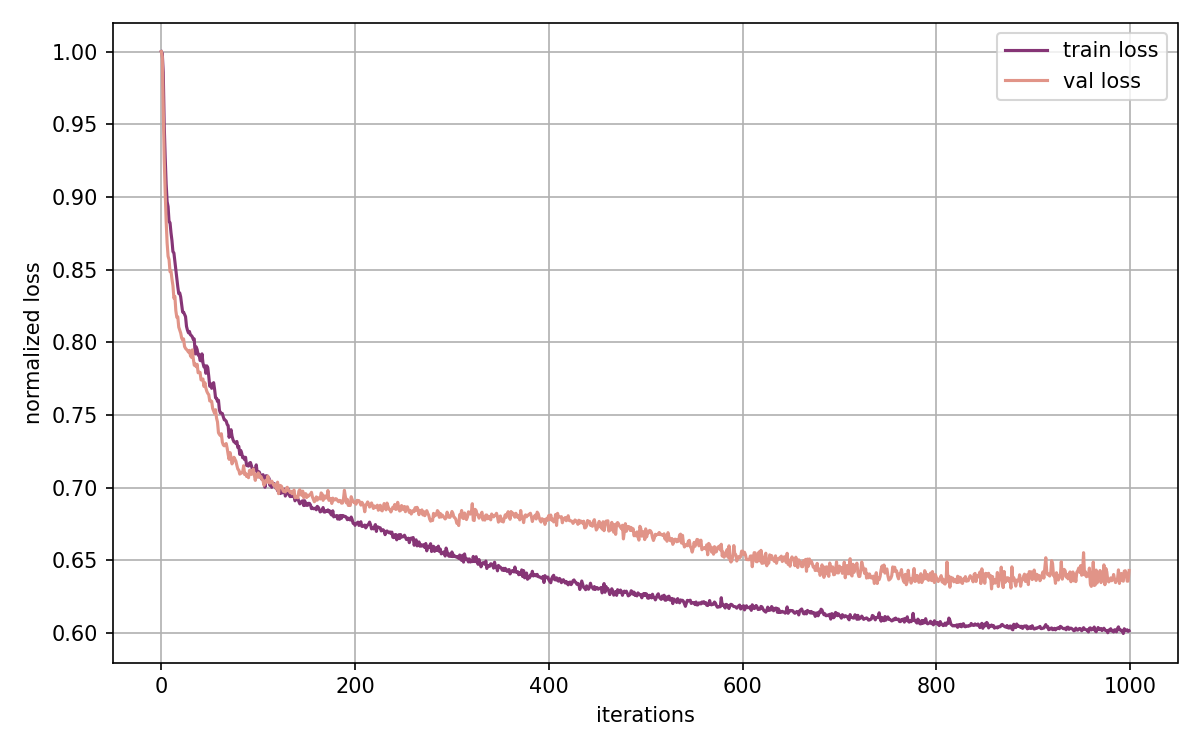
\includegraphics[width=0.45\textwidth]{./5_exp/figs/exp_adv_fc3_train_loss_random}}
  \caption{Comparing the train loss of L5-n500-norm1, c1d0dd0e0-norm1-it1000-bs32-lr0.0001-mo0.5 once with random init and once with adv init with dec-itl1000.}
  \label{fig:exp_adv_fc3_train_loss}
\end{figure}
\FloatBarrier
\noindent

\begin{figure}[!ht]
  \centering
    \subfigure[adv init]{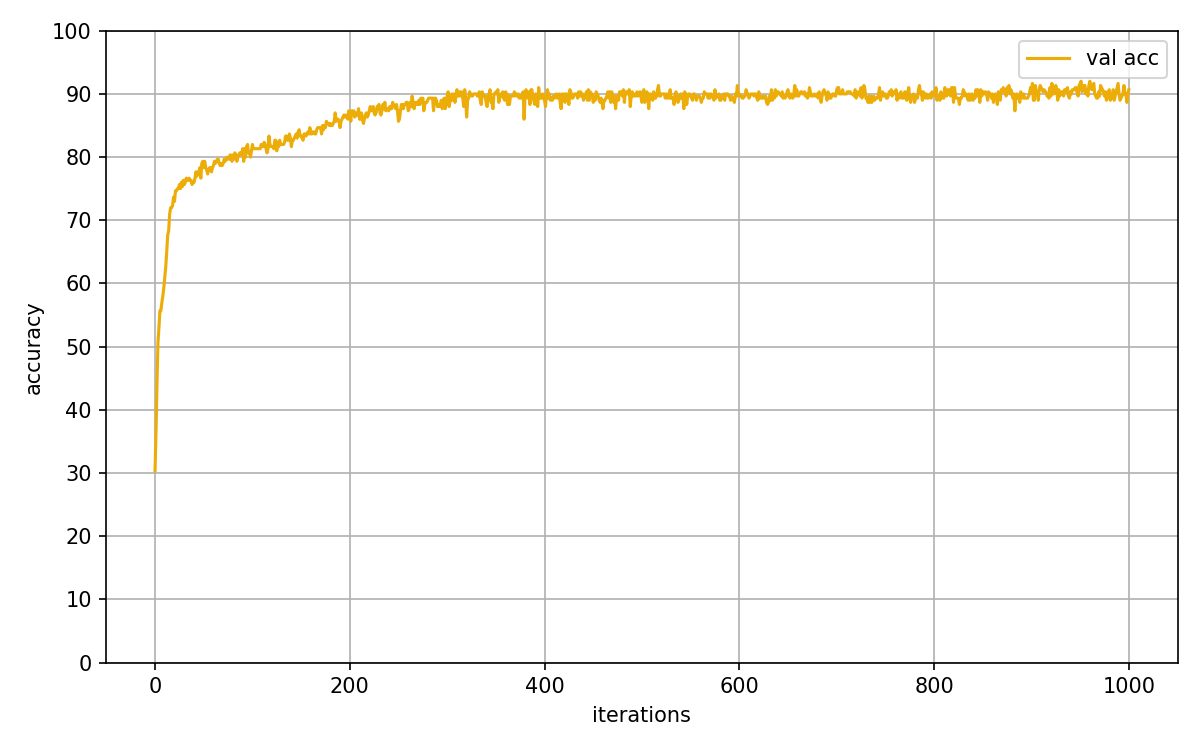
\includegraphics[width=0.45\textwidth]{./5_exp/figs/exp_adv_fc3_val_acc_label}}
    \subfigure[random init]{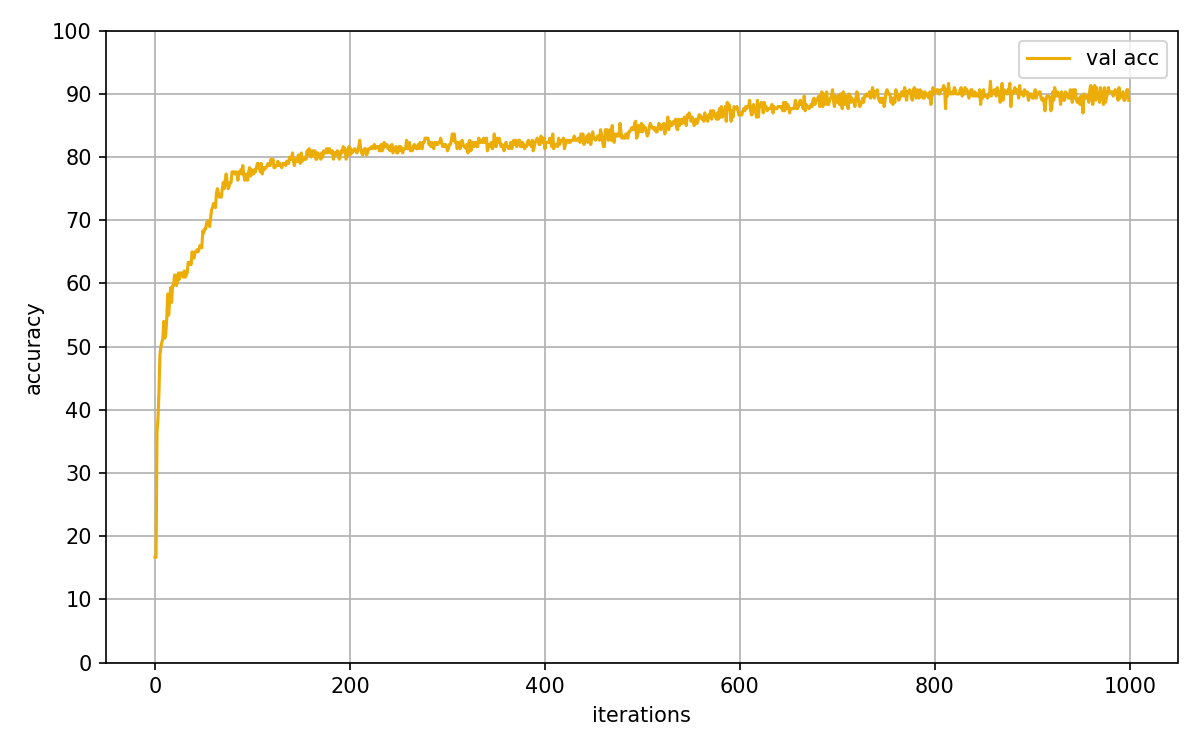
\includegraphics[width=0.45\textwidth]{./5_exp/figs/exp_adv_fc3_val_acc_random}}
  \caption{Comparing the validation accuracy of L5-n500, c1d0dd0e0-norm1-it1000-bs32-lr0.0001-mo0.5 once with random init and once with adv init with dec-itl1000.}
  \label{fig:exp_adv_fc3_val_acc}
\end{figure}
\FloatBarrier
\noindent

The loss and accuracy plots show how well the training was going forward for this showcase example. Both training work well and seem to converge, the one of the adversarial init parameters has a considerably faster convergence time here than the one without.
The scores on the test sets are shown in \rtab{exp_adv_fc3_score}, where both are achieving high scores on the test set, while the adversarial init one got a few percent more, but less on the my set.
This does not necessarily proof if one method is better or worse, therefore a more challenging task must be picked.
But at least it shows that adversarial pre training works at least as good as random initialization.
\begin{table}[ht!]
\begin{center}
\caption{Score comparison on arch: conv-encoder-fc3 with dataset: L5-n500 and training params: c1d0dd0e0-norm1-it1000-bs32-lr0.0001-mo0.5 and different adv params.}
\begin{tabular}{ M{2cm}  M{1.5cm}  M{1.5cm} }
\toprule
\textbf{adv params} & \textbf{acc test} & \textbf{acc my} \\
\midrule
none & 88.33 & 93.33 \\
dec-itl-1000 & 91.67 & 90.00 \\
\bottomrule
\label{tab:exp_adv_fc3_score}
\end{tabular}
\end{center}
\end{table}
\FloatBarrier
\noindent


\subsection{Wavenets}
Wavenets...
% --
% test bench

\section{Test Bench of best Neural Network Architectures}\label{sec:exp_tb}
\thesisStateNotReady
This section compares the best neural network architectures in terms of noise and shift invariance to fixed self recorded test audio files of the five speech commands with L5 labels.
The length of those audio files is cut, such that by applying a the fixed input frames of \SI{500}{\milli\second}, both end positions consists of at least the half of the audio file information.
This is especially important for the shift invariance.
The noise invariance finds the highest energy region, as described in \rsec{signal_raw} and uses this frame for classification.

% --
% shift invariance

\subsection{Shift invariances}
Shift invariances is very important for speech recognition, for instance the waveform should still be classified to the same class, when shifted a little bit in time.
However the restricted frame size of \SI{500}{\milli\second} makes this task very difficult, as it is already known that not all information might fit into the analytic window, like the \enquote{t} in \enquote{left} or \enquote{right} is often missed.
The figures in this section present a correct classification with a colored pixel and an incorrect with a white pixel.
The examples from the adversarial training section are shown in \rfig{exp_tb_shift_fc3}.
\begin{figure}[!ht]
  \centering
    \subfigure[adv init]{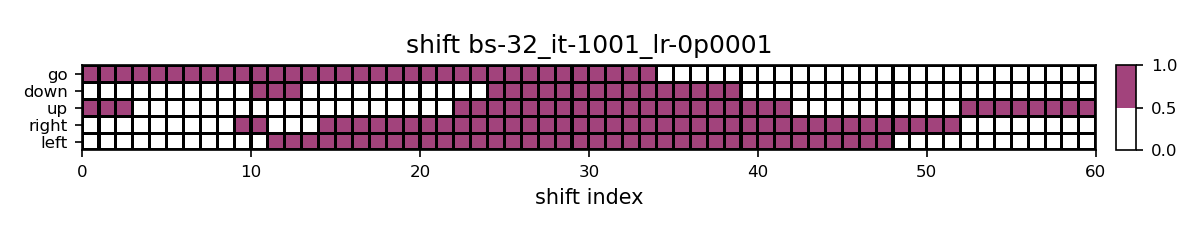
\includegraphics[width=0.45\textwidth]{./5_exp/figs/exp_tb_shift_fc3_adv}}
    \subfigure[random init]{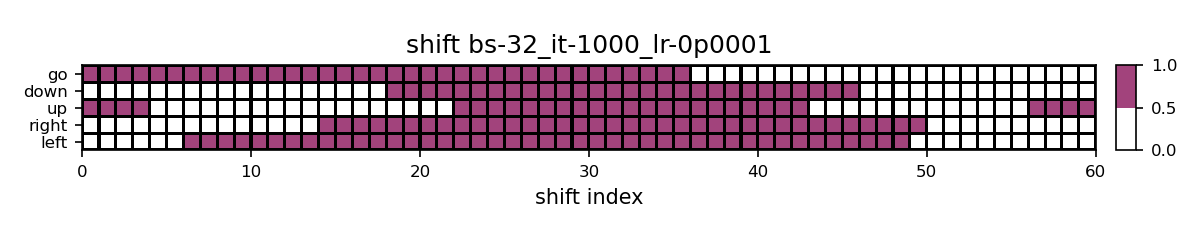
\includegraphics[width=0.45\textwidth]{./5_exp/figs/exp_tb_shift_fc3_random}}
  \caption{Shift invariance of L5-n500, c1d0dd0e0-norm1-it1000-bs32-lr0.0001-mo0.5 once with random init and once with adv init with dec-itl1000.}
  \label{fig:exp_tb_shift_fc3}
\end{figure}
\FloatBarrier
\noindent


% --
% noise invariance

\subsection{Noise invariances}
Noise invariance is a good trait in the classification of speech signals.
That is because the usage of bad microphones or recording set ups may add a lot of noise to the audio and therefore might disturb the classification accuracy.
To create a test upon noise invariance, artificial normal noise is added to the test audio files.
In the plots this is indicated in the x-axis of the plots as Signal to Noise Ration (SNR).
A SNR level of zero means there is equal energy of noise and signal, therefore this signal is already pretty much disturbed.
\rfig{exp_tb_noise_fc3} shows the noise invariance from the example in the adversarial training section.

\begin{figure}[!ht]
  \centering
    \subfigure[adv init]{\includegraphics[width=0.40\textwidth]{./5_exp/figs/exp_tb_noise_fc3_adv}}
    \subfigure[random init]{\includegraphics[width=0.40\textwidth]{./5_exp/figs/exp_tb_noise_fc3_random}}
  \caption{Noise invariance of L5-n500, c1d0dd0e0-norm1-it1000-bs32-lr0.0001-mo0.5 once with random init and once with adv init with dec-itl1000.}
  \label{fig:exp_tb_noise_fc3}
\end{figure}
\FloatBarrier
\noindent



% --
% game

\chapter{Video Games}
Video Games...
% --
% conclusion

\chapter{Conclusion}\label{sec:conclusion}
The conclusions concerns with the research questions asked in ...

% conclusions about best neural networks for video games

% conclusion about own experience in video games with kws

% answer of research questions


% --
% bib

% print bib
\printbibliography[heading=bibintoc]


\end{document}